\documentclass[degree=master, tocarialchapter]{thuthesis}
% 选项
%   degree=[bachelor|master|doctor|postdoctor], % 必选,学位类型
%   secret,                % 可选(默认:关闭),是否有密级
%   tocarialchapter,       % 可选(默认:关闭),章目录中使用黑体(这项表示同时打开下面两项)
%   tocarialchapterentry,  % 可选(默认:关闭),单独控制章标题在目录中使用黑体
%   tocarialchapterpage,   % 可选(默认:关闭),单独控制章页码在目录中使用黑体
%   pifootnote,            % 可选(默认:关闭),页脚编号采用 pifont 字体符号,建议打开

% 所有其它可能用到的包都统一放到这里了,可以根据自己的实际添加或者删除。
\usepackage{thuthesis}

% 定义所有的图片文件在 figures 子目录下
\graphicspath{{figures/}}

% 可以在这里修改配置文件中的定义。导言区可以使用中文。
% \def\myname{薛瑞尼}

\begin{document}

%%% 封面部分
\frontmatter
\thusetup{
  %******************************
  % 注意:
  %   1. 配置里面不要出现空行
  %   2. 不需要的配置信息可以删除
  %******************************
  %
  %=====
  % 秘级
  %=====
  secretlevel={秘密},
  secretyear={10},
  %
  %=========
  % 中文信息
  %=========
  ctitle={基于多步决策的文本情感识别},
  cdegree={工学硕士},
  cdepartment={计算机科学与技术系},
  cmajor={计算机科学与技术},
  cauthor={梁锡豪},
  csupervisor={徐明星副教授},
  % cassosupervisor={陈文光教授}, % 副指导老师
  % ccosupervisor={某某某教授}, % 联合指导老师
  % 日期自动使用当前时间,若需指定按如下方式修改:
  % cdate={超新星纪元},
  %
  % 博士后专有部分
  % cfirstdiscipline={计算机科学与技术},
  % cseconddiscipline={系统结构},
  % postdoctordate={2009年7月——2011年7月},
  % id={编号}, % 可以留空: id={},
  % udc={UDC}, % 可以留空
  % catalognumber={分类号}, % 可以留空
  %
  %=========
  % 英文信息
  %=========
  etitle={Multi-step-decision-making Based Text Sentiment Analysis},
  % 这块比较复杂,需要分情况讨论:
  % 1. 学术型硕士
  %    edegree:必须为Master of Arts或Master of Science(注意大小写)
  %             “哲学、文学、历史学、法学、教育学、艺术学门类,公共管理学科
  %              填写Master of Arts,其它填写Master of Science”
  %    emajor:“获得一级学科授权的学科填写一级学科名称,其它填写二级学科名称”
  % 2. 专业型硕士
  %    edegree:“填写专业学位英文名称全称”
  %    emajor:“工程硕士填写工程领域,其它专业学位不填写此项”
  % 3. 学术型博士
  %    edegree:Doctor of Philosophy(注意大小写)
  %    emajor:“获得一级学科授权的学科填写一级学科名称,其它填写二级学科名称”
  % 4. 专业型博士
  %    edegree:“填写专业学位英文名称全称”
  %    emajor:不填写此项
  edegree={Doctor of Engineering},
  emajor={Computer Science and Technology},
  eauthor={Liang Xihao},
  esupervisor={Professor Xu Mingxing},
  % eassosupervisor={Chen Wenguang},
  % 日期自动生成,若需指定按如下方式修改:
  % edate={December, 2005}
  %
  % 关键词用“英文逗号”分割
  ckeywords={情感分析, 反讽识别, 深度学习,集成学习},
  ekeywords={Sentiment analysis, irony detection, deep learning, ensemble learning}
}

% 定义中英文摘要和关键字
\begin{cabstract}

自Web2.0普及后,人们逐渐习惯在互联网的各种平台上分享他们的想法和情感。透过对这些媒体进行情感分析,我们可以得知人们对特定人事物的想法和态度。对人们的想法快速作出响应能够带来相应的商业价值和政治价值,其相关技术也因此得到了重视。而文本作为社交平台上的主要媒体之一,面向文本的情感识别在近年也成为了热门的研究领域。本论文探讨了文本情感识别中的两个问题,主要内容如下:

\begin{enumerate}

\item {\bf 基于多步决策的多分类系统框架}。随着现实中应用场景变得复杂,需要解决的多分类问题越来越多。当区分的类别越多,机器学习算法对数据进行拟合的难度更高,另外对识别性能的要求也变得复杂,譬如确保个别类别的召回率和正确率等。为此,我们提出了一种基于多步决策的多分类系统框架,把一个多分类问题拆解成多个子分类问题的叠加,再透过逐步回答每个子问题得出最终的识别结果。由于识别过程中每一步只关注一个子分类问题,我们能从局部调整系统的识别能力,并针对特定的评价指标进行优化。另一方面,每个子分类问题可以分别采用不同的算法,以此结合不同模型能捕捉到的不同信息。

\item {\bf 用于结合上下文的多通道模型}。在某些场景下,仅凭一段文本无法准确了解发言者想表达的意思和态度。为了处理这种情況,一些文本情感识別研究会引入上下文作为提示。为此我们提出了一种多通道模型框架,让对识别目标起不同作用的上下文先分别经过不同的编码器进行编码提取出有用的特征,再考虑合并正文和上下文的信息得出识别结果。

\end{enumerate}

为了验证基于多步决策的多分类系统框架,我们首先将其应用于面向微博的反讽识别,根据国际比赛SemEval-2018的任务三进行实验,结果显示我们的模型超过了当时排名第一的系统。
另外为了验证我们提出的多通道分类模型,我们将其应用于面向三轮对话的情感识别,根据公开比赛SemEval-2019的任务三进行实验,结果显示我们的模型达到了当时排名前十的性能。

% 关键词是为了文献标引工作、用以表示全文主要内容信息的单词或术语。关键词不超过 5
% 个,每个关键词中间用分号分隔。(模板作者注:关键词分隔符不用考虑,模板会自动处
% 理。英文关键词同理。)

\end{cabstract}

% 如果习惯关键字跟在摘要文字后面,可以用直接命令来设置,如下:
% \ckeywords{\TeX, \LaTeX, CJK, 模板, 论文}

\begin{eabstract}

Since the poularization of Web 2.0, people get used to share they thoughts and emotions on different online platforms. By analyzing the sentiment of these data, we can have an in sight into the people's opinion towards certain things. Vast commercial and political values can be obtained through quick response to the people's attitude. Therefore related technologies are getting more attention. As text is one of the mostly used media on social platforms, text sentiment analysis has become a popular research field. This thesis explores two problems in text sentiment analysis and it is organized as follows:

\begin{enumerate}

\item {\bf Multi-step-decision-making based multi-classification system framework}. As real-world application scenes are becoming more complex, more multi-classification problems are encountered. As the data are divided into more categories, it becomes more difficult for machine learning algorithms to fit the data. On the other hand, the requirement of predictive performance are getting more complicated, such as ensuring the recall rate and the precision level of certain categories. Hence, we propose a multi-step-decision-making based multi-classification system framework, which disassembles a multi-classification problem into a sequence of sub-classification problems and classifies an object by answering the sub-questions step by step. As the classification system only focuses on a sub-problem at each step, its performance can be adjusted locally and we can optimize the overall performance for certain evaluation metrics. On the other hand, algorithms can be chosen for each sub-problem individually, hence the information captured by different kinds of models can be combined in the system.

\item {\bf Multi-channel model for manipulating contextual information}. Sometimes we may not exactly understand what a person want to express or how he feels only through his written message. To deal with this problem, some of the text sentiment analysis researches take into account the contextual clues. Therefore, we propose a multi-channel model. By feeding contextual information that play different parts of role into different feature encoders, features of different parts of the context are encoded and further combined with that of the main message to get the identification result.

\end{enumerate}

To verify the effectiveness of the proposed multi-step-decision-making based multi-classification system framework, we first apply it to irony detection in English tweets. Experiments are launched based on SemEval-2018 Task 3. Results show that our system exceeds the performance of the no. 1 participating system. On the other hand, to verify the effectiveness of our multi-channel model, we apply it to contextual emotion detection in text. Experiments are launched based on SemEval-2019 Task 3. Results show that our system reaches the top 10 performance among the participants.

\end{eabstract}

% \ekeywords{\TeX, \LaTeX, CJK, template, thesis}

% 如果使用授权说明扫描页,将可选参数中指定为扫描得到的 PDF 文件名,例如:
% \makecover[scan-auth.pdf]
\makecover

%% 目录
\tableofcontents

%% 符号对照表
\begin{denotation}[3cm]

\item[BOW] 词袋模型 (Bag of Words)
\item[BP] 反向传播算法 (Back-propagation)
\item[BRNN] 双向递归神经网络 (Bidirectional Recurrent Neural Network)
\item[CRF] 条件随机场 (Conditional Random Field)
\item[GRU] 门控循环神经元 (Gated Recurrent Unit)
\item[LSTM] 长短时记忆网络 (Long Short-Term Memory)
\item[POS] 词性 (Part-of-speech)
\item[RNN] 递归神经网络 (Recurrent Neural Network)
\item[SVD] 奇异值分解 (Singular Value Decomposition)
\item[SVM] 高性能计算 (High Performance Computing)
\item[TF-IDF] 词频-逆文档频度 (Term Frequency - Inverse Document Frequency)
\item[ReLU] 线性整流函数 (Rectified Linear Unit)

\end{denotation}



%%% 正文部分
\mainmatter
\chapter{引言}
\label{cha:intro}

\section{研究背景与意义}

情感识别旨在了解人们对特定事件或实体的态度和情感。自Web2.0普及后,大量网民每天在互联网生产着各种各样的内容,其中包含不同方面的信息,如个人生活经历,购买行为,对产品服务的体验评价,对社会时事的看法等等。从人们的日常社交需求来看,这种借由互联网媒体的分享非常便捷,我们可以了解到亲朋好友的近况,也可以和不认识的网民交流对具体事件的想法。在商业上,借由对用户的网络行为进行分析,企业可以对他们的客户或者潜在客户有更深入的了解,对他们的需求和反馈及时作出反应将带来战略性的优势。在社会管理上,政府可以透过对网民在网络上的发言了解人民的想法和舆论的走向,进而作出相应的措施。正因为互联网的普及,才使得以上基于对特定人群的了解来进行决策的做法成为可能。随着数据资源变得丰富,相应的技术在近年得以快速发展,目前市面上已经有公司(如国内的腾讯和阿里巴巴,以及国外的微软和亚马逊等)提供基于大型社交媒体平台(如微博、讨论区等)上的数据进行情感分析相关的规泛化服务,然而相应的技术依然有进步空间,研究工作还在不同方向上摸索。

情感在人们的思想表达和交流中起着重要作用\cite{Banerjee2015Detection},比起了解该想法的细节内容,情感对应该想法的一种倾向。譬如在分析用户对新产品的评论时,
只需要分析其中褒贬意思的倾向即可大致了解新产品是否能让大部分的客户满意,或者筛选出其中表示不满意的用户再进行深入分析,因此情感识别技术具有一定的应用价值。而由于在互联网上,大部分情况下用户以文本表达想法,面向文本的情感识别成为了近年最重要的研究课题之一。相对于人们面对面交流的场景,聆听者可以根据发言者的肢体语言、面部表情以及声调变化等额外信息更好地理解发言者想表达的意思,然而这些信息并不存在于文本当中,这也正是对文本进行情感识别本身的难点之一\cite{SemEval2019Task3}。

情感识别的另一个难点在于语言中丰富多样的修辞手法,其中反讽是具代表性的修辞手法之一。Henry Watson Fowler在《The King's English》一书中描述“即使对反讽的定义有数百种, 其中只有包含'表面意思和实际意思不同'这个概念的才能被接受”。Eric Partridge 在《Usage and Abusage》一书中指出“反讽存在于所表达意思的另一面”。总的多说当反讽在文本中出现,那么发言者想表达的意思应该和文本的字面意思完全相反。譬如某人表示“我就喜欢你不断挑战我的底线”,在字面上“喜欢”表达的是正面的情感,然而根据常识可知“挑战底线”是一种让人反感的行为,与“喜欢”相矛盾。这段文字实则表示发言者正被某人触及底线,表达的是负面情感。所以在情感识别当中,正确识别出反讽的使用能够避免对内容的错误理解,反讽识别因此成为了和情感识别紧密相关的研究课题。

\section{国内外研究现状}

\subsection{情感模型}

情感计算的基础是对情感作出描述,现有的描述方式可以分成两个大类: 范畴观和维度观。范畴观即把不同情感对应到一组离散的情感标签上,其中具代表性的有Plutchik的情感模型\cite{Plutchik1980Emo}和Ekan的情感理论\cite{Ekman1992An}。Plutchik的情感模型包含八种情感:愤怒、恐惧、悲伤、厌恶、期待、信任、高兴、惊讶;这些情感都各自对应具有重要生存意义的行为,各种复杂的情感都是由这此基本情感构成,另外这八种情感可以分成四组对立的情感对。Ekan在十年后提出的情感理论和Plutchik的相似,但相对地少了期待和信任两种情感,是一个六类情感模型。

\begin{figure}[h]
  \centering%
  \subcaptionbox{三维模型\label{fig:plutchik_emotion_wheel_3d}} %[3cm] 标题的长度,超过则会换行,如下一个小图。
    {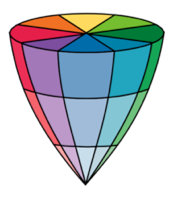
\includegraphics[height=4cm]{img/plutchik_3d.png}}%
  \hspace{4em}%
  \subcaptionbox{二维模型\label{fig:plutchik_emotion_wheel_2d}}
      {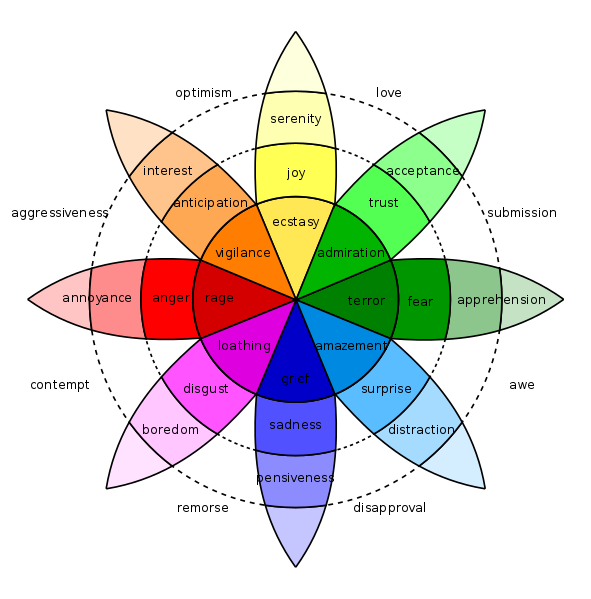
\includegraphics[height=8cm]{img/plutchik_2d.png}}
  \caption{Plutchik\cite{Plutchik1980Emo}提出的情感轮模型}
  \label{fig:plutchik_emotion_wheel}
\end{figure}

以维度观描述情感就是把情感映射到多维空间的点上,而目前维度观情感模型以二维和三维空间的为主。二维情感模型中较有代表性的是Russell提出的环状模型(Circumplex Model)\cite{Russell1980Cir} ,其中纵坐标对应情感的激活度(Arousal),横坐标对应情感向性(Valence),而不同的情感则分布在一个环状的区域内。Bradley等人\cite{Bradley1992Rem}提出的向量模型(Vector Model)在对横轴和纵轴的定义和前者相似,但其理论假设高激活度的情感应该有较明显的正负倾向,相对地低激活度的情感则偏向中性,故情感分布在一个回力标形状的区域。Watson和Tellegen \cite{Watson1985Tow} 提出的 PANA(positive activiation-negative activation)模型和前两者在理论基础上则有明显的不同,他们认为情感的正面作面和负面作用是两个独立的成分,所以在模型中纵轴和横轴分别表示情感正面作用和负面作用的强弱,不过该模型相当于把Russell等人提出的环状模型的向量空间旋转45度\cite{Rubin2009A}。

基于三维空间的情感模型中具有代表性的有Plutchik\cite{Plutchik1980Emo}提出的情感轮模型,Plutchik认为情绪之间包含强度,相似性和两极性三种维度,椎体的顶部和底部分别对应强的情感和弱的情感,相似的情感对应椎体中相近的位置,对立的的情绪则会对应到椎体中对立的位置上。另外还有Mehrabian \cite{Mehrabian1996Pleasure}提出的PAD模型,其三维空间的三个坐标轴分别对应情感愉悦度(Pleasure)、激活度(Arousal)以及优势度(Dominance)。较近期被提出的是Hugo\cite{Hugo2012A}的情感立方体模型,其三维空间的三个坐标轴分别对应5-羟色胺(5-hydroxytryptamine, 5-HT), 多巴胺(dopamine,DA)和去甲肾上腺素(noradrenaline,NE)三种神经递质所产生信号的强弱,并对空间中一个立方体的八个顶点标记了其对应的情感。

\begin{figure}[H] % use float package if you want it here
  \centering
  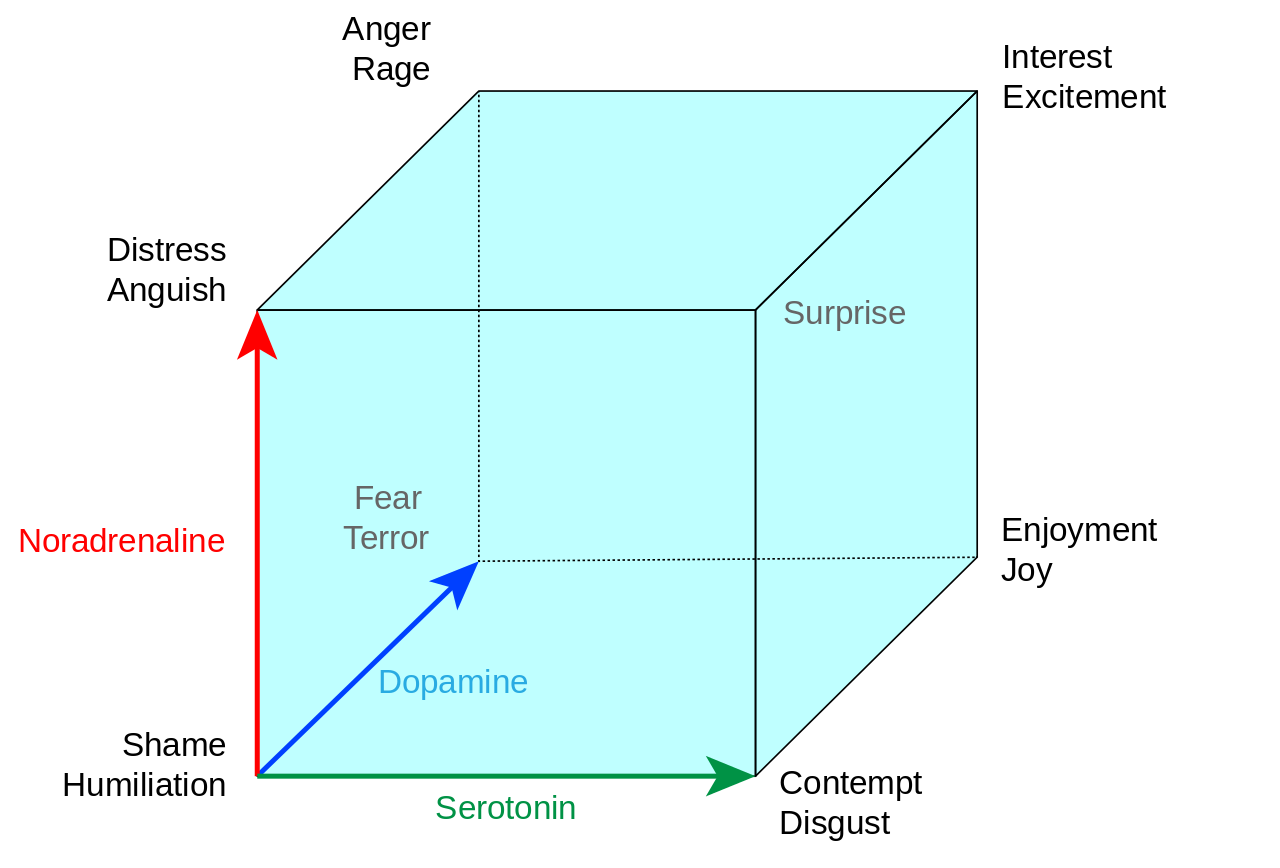
\includegraphics[width=0.8\textwidth]{img/hugo_cube_of_emotion.png}
  \caption{Hugo\cite{Hugo2012A}提出的情感立方体模型}
  \label{fig:hugo_cube_of_emotion}
\end{figure}

\subsection{情感识别}

对应上述情感模型的分类,情感识别研究可以分成两类。第一类对应范畴观,给定一组情感类型,判断一段文本中所表达的情感倾向于该组情感中的哪一种,或者是否包含这一组情感中的一种或多种情感。如国际比赛SemEval-2018任务一\cite{mohammad2018semeval}的子任务要求识别一段微博中是否包含愤怒、恐惧、悲伤等十一种情感中的一种或多种情感。另一类情感识别研究对应维度观,对于给定的情感属性,判断一段文本中该情感属性的强度。其中常见的有情感向性的二分类问题(正性或负性)、三分类问题(正性、中性或负性)、五分类问题(非常正性,正性、中性、负性或非常负性)。其中五分类问题的研究对象一般是互联网上五星评分制的产品评论或者电影评论等。

另一方面,目前文本情感识别的研究按照文本的粒度可以大致分成三类:文章级别、句子级别、属性级别。在文章级别的情感识别中,虽然一篇文章由多个句子组成,但假设整篇文章存在某种情感倾向,而研究目标则是自动识别出该种情感倾向的类型或强度。Turney \cite{turney2002thumbs} 利用线上电影评论中"推荐"(大拇指朝上)和"不推荐"(大拇指朝下)的标记研究对电影评论的正负性情感识别。他提出利用点互信息(Pointwise Mutual Information,PMI)来评估单词的语义倾向性,其中PMI透过在大型语料库中统计两个单词共同出现的情况来评估两个单词的相似度。首先利用PMI值评估各个单词与正向情感的代表性单词"excellent"和负向情感的代表性单词"poor"的相似性,再取这两个PMI值作差得出该单词在语义上倾向于哪一种情感,再透过计算整段评论的平均语义倾向性评估整体的情感倾向。Pang和Lee \cite{pang2004sentimental} 采用了不同的方法研究相同的问题。他们首先对评论中每个句子的主观程度进行评分,利用评分构造一个带权重的句子关系图,再基于最小割算法结合上下文加强对每个句子主观程度的判断,过滤评论中不带主观情感的句子后再判断整个评论的情感向性,以此加强识别效果。Tang等人 \cite{tang2015learning} 则研究了产品评论的五级评分预测。除了评论的文本内容,他们进一步引入了用户的信息和产品的信息。经过数据分析,他们发现相同用户对不同产品的评论和评分比不同用户之间的更一致,另外不同用户对同一产品的评论和评分比不同产品之间的更一致,这显示了用户和产品各自都存在一些相对固定的属性。因此Tang等人提出一种为用户和产品生成表示向量的方法,并应用于评论的五级评分预测。实验结果显示他们的方法在多个数据集上达到了较好的性能,这同时引出了加入背景信息来加强系统识别能力的可能性。

然而一篇文章有可能同时表达了多种观点和情感,因此有另一类研究针对句子或短文本所表达的情感,即句子级别的情感识别。由于句子的文本长度较文章的短,文本内部的逻辑较简单,但相对地所包含的提示信息也较少,课题的难点与前者有所不同。Khan等人\cite{khan2011sentiment}研究了对线上评论中句子进行正负性情感识别。他们首先区分出评论中各个句子的主观性和客观性,然后针对带主观情感的句子,利用开源自然语言工具SentiWordNet获取各个单词的正负情感属性,再根据句子的词性标注和他们设计的规则计算整个句子的情感向性。Khan等人默认单词的正负情感属性在不同场景下不变,然而Li等人\cite{li2013constructing}指出部分单词在特定场景下会有不同的情感向性,因此他们提出了一种有监督学习方法,自动学习各单词在指定领域下的情感向性,以此作为文本的特征,并应用于对产品评论的情感识别中。实验结果显示使用SentiWordNet提供的全局情感评分和针对领域评估的情感评分相比,使用后者能达到的识别性能力更好,验证了他们的假设。一些研究则选择端到端地学习单词的情感和语义倾向,在Santos和Gatti\cite{dos2014deep}对电影评论和微博的情感识别研究中,他们提出了利用卷积神经网络分别从字符级别和词级别计算出单词对应的特征向量,然后同样以卷积神经网络结合句子中各单词的向量得出句子的表示向量和预测整体的情感倾向。结果显示他们的方法较早期的其他方法性能更好。

在一些应用场景当中,我们希望了解发言者对某个对象或者它的某个特定属性的想法。譬如新手机推出市场后,厂商需要了解用户对手机的续航能力、拍照质量、交互体验等各方面的评价,那么对于评论中同时谈论手机的多个属性且好评和差评不一时,应该针对各个属性分别识别发言者所表达的感情,因此有了属性级别的情感识别。Che等人\cite{che2015sentence}提出一种句子压缩算法,透过对句子进行依存句法分析,过滤与目标属性的情感无关的内容。他们采用了多种语义和语法特征作为输入,以条件随机场(Conditional random field,CRF)作为分类器。实验结果显示过滤掉不相关的文本部分后,识别性能有所提升。Wang等人\cite{wang2016attention}研究了对网上评论中特定实体或属性的情感识别。他们提出了一个基于注意力机制的长短时记忆网络(Long Short-Term Memory,LSTM),特点在于只以词向量作为输入,而不采用其他传统的语义和语法特征,另外利用注意力机制自动识别与目标相关的内容。他们的实验基于国际比赛SemEval-2014任务四\cite{pontiki2014semeval}中的一个子任务,结果然显示他们的系统性能达到了当时的技术水平。另外透过对注意力单元的输出进行分析,验证了注意力机制能够有效识别文本中与目标相关的内容。Tang等人\cite{tang2016aspect}分别对前述数据集中电脑和餐庁相关的两组样本进行属性级别的情感识别,但有别于当时主流的以特征提取为主的浅层机器学习方法(如支持向量机)和针对序列的深度学习模型(如递归神经网络),他们提出了一个基于注意力机制的深度记忆网络。另外针对文本中各个单词和目标单词在句子中的距离,作者引入了距离信息提出了注意力单元的多种变形。实验结果显示他们提出的深度记忆网络达到了当时第一名参赛系统(基于手工特征和支持向量机的算法)的性能。另外对注意力单元的中间结果进行人工分析,验证了在同一段评论中,引入距离信息的注意力单元有助于区分不同单词对不同目标的情感的贡献。

\subsection{反讽识别}

正如前面所述,反讽识别和情感识别紧密相关,识别出反讽的使用对正确识别情感起着关键作用。Tsur等人\cite{tsur2010icwsm}\cite{davidov2010semi}研究了对微博平台Twitter上的微博以及电商平台亚马逊上的评论进行反讽强度的识别,从明显不含反讽到明显表示反讽分成五级,由人工进行标注。他们提出的SASI算法分别从文本提取了词频相关的模式特征以及基于标点符号的特征,以K最近邻算法作为分类器。另外利用在Twitter按井号标签\#sarcastic自动爬取了额外的反讽语料用于初步的模型训练。对实验结果的比较证明了各种特征的有效性以及添加额外语料对模型训练的帮助。

为了以较低成本获取大量的反讽相关语料,很多研究从微博平台根据井号标签自动筛选出可能带反讽的微博。Reyes等人 \cite{reyes2013multidimensional} 利用\#irony,\#education, \#humor, \#politics在Twitter上自动获取四组不同主题的微博,并把\#irony对应的微博和另外三组微博两两组合进行二分类实验。他们提出了四个方面的文本特征提取方法,包括:特殊标记(词汇和标点符号等)、不可预期性、表达风格、情感特性;并比较了每项特征在各组微博中的出现情况,显示了各项特征和反讽的相关性。另外分别采用朴素贝叶斯和决策树作为分类器,但没有明显的性能区别。

类似的数据收集方法对其他语言同样适用。Kunneman等人\cite{kunneman2015signaling}则利用对应的德语井号标签来获取反讽语料,以此研究德语微博中的反讽识别。他们取N元语法作为输入特征,以Balanced Winnow \cite{littlestone1988learning}作为分类器,在测试集上达到约0.85的召回率和0.87的AUC值。但他们进一步经过人工检验评估了基于井号标签自动标注的有效性,分析结果显示该方法获取的反讽样本中包含约10\%的躁声。

有别于早期以手动设计的特征作为输入和以传统机器学习方法建模,Poria等人 \cite{poria2016deeper} 首次将神经网络应用于对微博的反讽识别。他们的算法框架主要包含四个卷积神经网络,并分别利用不同的数据集进行预训练,分别对应反讽识别、情感极性识别、情感类型识别和性格识别。最后取四个卷积神经网络的中间结果作为特征,利用支持向量机(Support Vector Machine, SVM)进行后融后得出最终预测结果。实验显示引入反讽识别以外的三个语料库提升了系统的识别能力。

\begin{figure}[H] % use float package if you want it here
  \centering
  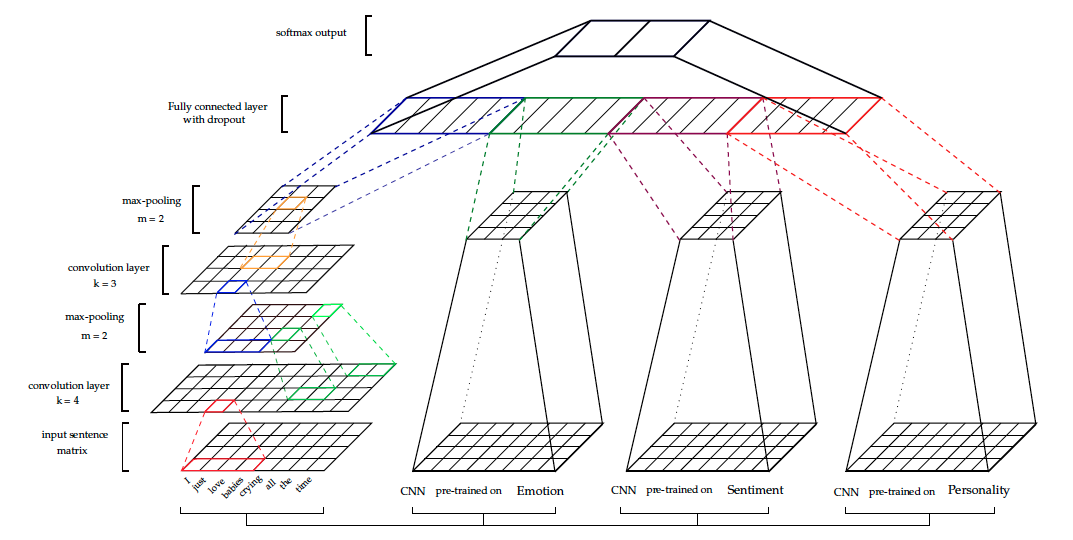
\includegraphics[width=\textwidth]{img/poria2016deeper.png}
  \caption{引入多个领域信息的反讽识别神经网络模型,引自\cite{poria2016deeper}}
  \label{fig:poria2016deeper}
\end{figure}

\subsection{社交媒体上的文本情感识别}

随着社交媒体的普及,网民们习惯于在微博、讨论区等平台上表达个人意见和互相讨论。有别于新闻或学术材料等较正式的文件,网民可以较随心所欲地发言,社交媒体因此成为了情感识别的重要研究对象之一。但和产品评论或文章等文本类型不同,社交媒体上的文本普遍较短\cite{Madhusudhanan2018survey},缺少对背景信息的提示,难以判断其内容所属的主题,这对正确理解其中表达的意思带来困难。另外语言中夹杂着不正规的用法,在中文微博中会出现新的短语或对旧短语有新的解释\cite{xie2012jiyu},如“锦鲤”暗示“好运”,“灌水”表示发表没有意义的内容,在英文微博则中会出现错拼字、非正式缩略语、表情符\cite{go2009twitter}\cite{paltoglou2012twitter},如“tnx”对应英文单词“thanks”,“:)”表示微笑等。虽然没有正式的语言组织对这些新的用法进行整合,但因为这些新用法更方便或对思想的表达更丰富到位,随着在网络上的传播而在网民之间达成了共识。传统的文本特征提取建立在标准的单词使用和正规的语法结构上,而由于新词汇和新语用的出现,导致词汇的意思无法被识别或被错误理解,这对于由人工智能理解文本内容成为了一大难点。因此有别于传统的文本研究,在面向社交媒体的文本情感识别时,需要采用额外手段对文本进行预处理,或透过大量语料尝试自动学习这些新出现的语言属性。

Khan等人\cite{khan2014tom}研究了微博的正负中性情感识别。他们提出了一个混合三个分类器的情感识别框架来解决数据稀疏的问题,另外还提出了一组针对微博文本的预处理步骤,其中包括俚语和缩略语分析、词干提取、拼写检查和修正、用户名和井号标签移除等。他们的系统在6个微博数据集上达到了平均83.3\%的F1值以及平均85.7\%的准确率,和同类型技术比较后验证了他们系统以及预处理手段的有效性。

Angiani等人\cite{angiani2016comparison}针对英语微博比较了各种常用的文本预处理技术对情感分析的影响,其中包括单词的规范化、表情符到情感标签的映射、俚语映射、词干提取、停词过滤等。分析显示除了俚语映射以外,其他技术均对情感识别都有正面影响,其中部分技术有助于统一拼写相似的单词,以此关联相同概念的词组。但同时采用所以预处理技术并不保证达到最好的效果,作者指出依然需要根据应用场景和文本的特性做选择。

\begin{figure}[H] % use float package if you want it here
  \centering
  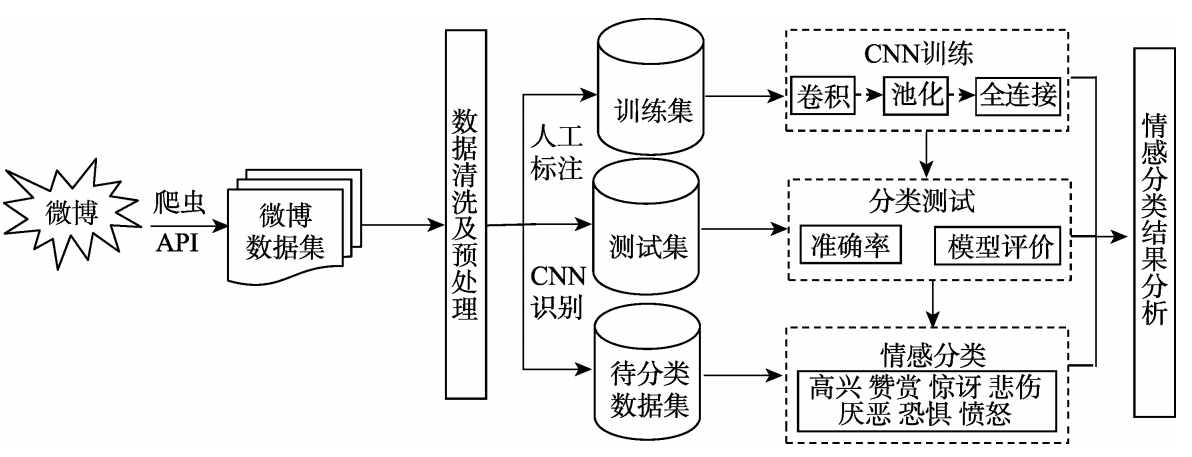
\includegraphics[width=0.8\textwidth]{img/zhang2018jiyu.png}
  \caption{基于卷积神经网络的微博情感分类模型,引自\cite{zhang2018jiyu}}
  \label{fig:zhang2018jiyu}
\end{figure}

张海涛等人\cite{zhang2018jiyu}则研究了中文微博和评论中的文本情感分类。他们针对当时微博上具一定争议性的话题\#打呼噜被室友群殴\#收集数据,确保了样本围绕同一个主题并且有充足的数据量。使用开源工具 NLPIR/ICTCLAS2016 对语料进行分词,再以词向量学习算法word2vec从语料中学习词的表示向量作为输入,以基于卷积神经网络的模型作为分类器,另外以支持向量机作为对照算法。实验结果显示在面向长文本的情感识别时,他们的系统比支持向量机性能更好,而面向短文本时则相反。

\section{存在的问题}

由于近年来各企业或机构对情感识别的需求增加,相关技术的研究备受关注,加上深度学习的快速发展,情感识别和反讽识别的性能水平也在逐年提升。然而相关研究依然存在一些问题需要深入探讨:

\begin{itemize}

\item {\bf 数据不均匀在多分类问题中的影响}。情感识别在早期以识别文本的正性、负性和中性情感为主,但随着应用场景越来越复杂,相关研究逐渐关注其中的细分类别,反讽识别等研究也如此。而在多分类问题中,各类别样本量分布不均匀一直是个备受关注的问题。因为在真实应用场景的多分类问题中,各个类别的样本量往往分布不均匀甚至差别很大,这会导致部分性能指标明显偏低。譬如在训练数据中样本量较少的类别在测试集上的召回率会明显比其他类别的低,间接拉低宏平均的召回率和F1值。然而目前主流的研究工作大部分只探索单个模型如何对多类别的数据进行建模,在人工神经网络领域则是不断提出新的网络结构以在整体上达得到更好的识别能力。另外也有透过数据增强的方法调整训练数据中样本的分布情况,但也难以针对个别类别的识别能力进行调整。

\item {\bf 在算法建模中引入上下文信息} 在一些场景下,仅凭一段文本的内容可能无法完全理解发言者想表达的内容,这在短文本的场景中尤其明显,如微博、评论等。为此目前一些研究会考虑引入文本的上下文,认为这些上下文中包含相关的信息,有助于理解原文的内容。但在不同场景下,上下文的类型不同,其对应建模方式也会有所不同。如在微博平台中,要对微博正文进行情感识别,那么可以引入微博底下的评论以定位该微博描述的事情,另一方面也可以引入用户过去发布的微博,对比他使用表情符的习惯和当前微博中使用的表情符来猜测用户想表达的情感。然而对于不同场景下不同类型的上下文,如何在算法建模中引入上下文信息始终没有一种通用的方法,对于具体的问题依然需要进行针对性的设计。

\end{itemize}

\section{本论文的内容安排}

本文针对上述的两个问题,提出了一个基于多步决策的多分类系统框架以及用于结合上下文的多通道分类模型,并分别基于两个应用场景进行实验以验证他们的有效性。本论文的内容安排如下。

在第\ref{cha:problem_framework}章,我们会对面向文本的情感识别问题作出分析,给出一个统一的数学定义。然后我们会给出一个文本情感识别的研究框架,详细说明其中每一步完成的任务和目的。紧接着会介绍一些自然语言处理和情感识别的相关技术,对于后续实验用中使用到的技术,我们会给出相对充分的说明,另外也会给出相关技术的概要描述,以便于其他研究者在本论文未深入探索的方向进行拓展性的工作。

第\ref{cha:exp_irony_det}章中,我们针对面向微博的反讽识别提出了一种多分类器分层识别算法,同时引出一种针对多分类问题的算法设计框架。我们将基于国际比赛SemEval-2018的任务三\cite{van2018semeval}展开实验,其中包含两个子任务。子任务一为二分类问题,要求识别微博是否包含反讽的修辞手法。另一个子任务为四分类问题,数据与子任务一相同,但原本"反讽"一类的样本被细分成反讽的三个类型:基于相反语义的反讽、情景反讽、其他反讽。我们提出的多分类器分层识别算法面向子任务二的四分类问题,我们会首先对组成该算法的子模型进行分析,再对整个算法的最终识别结果和中间结果进行分析,以此验证算法的有效性以及其设计的合理性。最后进行错误分析,了解我们的算法在此研究问题中的不足之处。

在第\ref{cha:exp_context_emo}章,我们提出了一种多通道分类模型,用于结合在情感识别中起着不同作用的上下文信息。基于此多通道分类模型,我们再给出了一个和前一章的算法框架相似的多分类器分层情感识别算法,并应用于面向三轮对话的情感识别。我们将基于国际比赛SemEval-2019的任务三\cite{SemEval2019Task3}展开实验,该比赛要求参赛系统识别两人轮流发言的三轮对话中最后一轮发言者所表达的情感,一共涉及四个情感类别:高兴、悲伤、愤怒、其他。
同样地,我们会对组成该算法的子模型进行分析,再对整个算法的最终识别结果和中间结果进行分析,一方面验证算法的有效性以及其设计的合理性,另一方面验证我们提出的多分类器分层识别算法框架在不同多分类问题上的通用性。

最后,在第\ref{cha:conclusion}章中,我们将总结本篇论文中的主要贡献和实验结论,并根据前面各实验的错误分析为后续研究工作给出建议。













\chapter{问题分析和研究框架}
\label{cha:problem_framework}

\section{本章引论}

随着互联网上不同类型的平台出现,人们每天在各种平台上产生着各种各样的行为和发言。如现在微博平台上会对热门时事设置井号标签,人们透过加上对应标签来表达对该事件的想法,以及透过对这些发言进行赞点、分享或评论来表达支持或反驳。利用井号标签收集数据并进行意图分析可以得知网民对该事件的舆论方向。在其他平台上的各种行为记录同样可能有挖掘其意图的价值,意图识别的应用场景也变得多种多样,但即使数据的内容和结构不同,问题的本质是相似的。

本章的内容安排如下。在章节\ref{sec:global_problem_analysis}中,我们将首先针对意图识别进行分析,并给出统一的形式化表示。基于该形式化表示,在章节\ref{sec:global_framework}中,我们再进一步提出一个面向社交媒体文本的意图识别研究框架。从原始文本的输入到最终识别目标的输出,理清其中每个步骤的功能和目的,给出一个完整识别系统的设计方案,为解决后续章节中研究的问题准备一个统一的切入点。

\section{问题分析}
\label{sec:global_problem_analysis}

本小节中,我们将对意图识别中涉及的各个元素作出分析,并给出统一的形式化表示来描述他们的相互关系。

不同意图识别问题中都有要被识别的意图倾向$C$。如Tang等人\cite{tang2015learning}的情感极性识别研究,$C$对应需要五级的情感极性。在刘丹丹等人\cite{刘丹丹2015基于}的微博情感分类研究中,$C$对应喜好、安乐、惊奇、厌恶、悲哀、愤恨、恐惧。邓钊等人\cite{2015面向微博的中文反语识别研究}的中文反语识别研究中,$C$则对应是否包含反讽。

其次是研究主体$T$,它是行为发起者$S$的行为记录,可以认为他表达想法和情感的载体。另外一些场景下会有背景信息$B$,对应所有有助于正确理解$T$的信息。譬如要研究讨论区上帖子的意图倾向,那么$T$就是帖子的内容,包括其中的文本内容、图片、文件附件等,$S$则是帖子的发布者。而帖子所在讨论区的类型有助于定位帖子对应的领域,发布者的发布历史显示发布者的一些态度倾向,帖子下的评论从侧表反映主帖的内容,这些就是背景信息$B$,都可能是理解帖子内容的提示。又以Zahiri等人\cite{Zahiri2017Emotion}对电视剧台词的情感识别研究为例,那么$T$指电视剧中的台词,$S$则是发出这段台词的对应角色,$B$则是台词的上文,其中包含其他角色正在谈论的内容,这些角色和发言者的关系是什么,说话的氛围如何等等,都能对台词的内容有更明确的定位。

意图识别假设对于任意一个研究样本$t \in T$,在给定背景信息$b \in B$(或某些情况下假设与背景信息无关),其承载想法或情感必然存在对应的倾向$c \in C$。意图识别首先要从样本主体和背景信息中分别提取出与识别目标相关的信息$f_t$和$f_b$,即需要提出两个映射函数,$F_T$和$F_B$,满足 $f_t=F_T(t)$和$f_b=F_B(b)$。再进一步根据相关信息识别出其想法或情感倾向,即找出一个映射关系$F_C$,使得 $c=F_C(f_t, f_b)=F_C(F_T(t), F_B(b))$。

\begin{figure}[H]
  \centering
  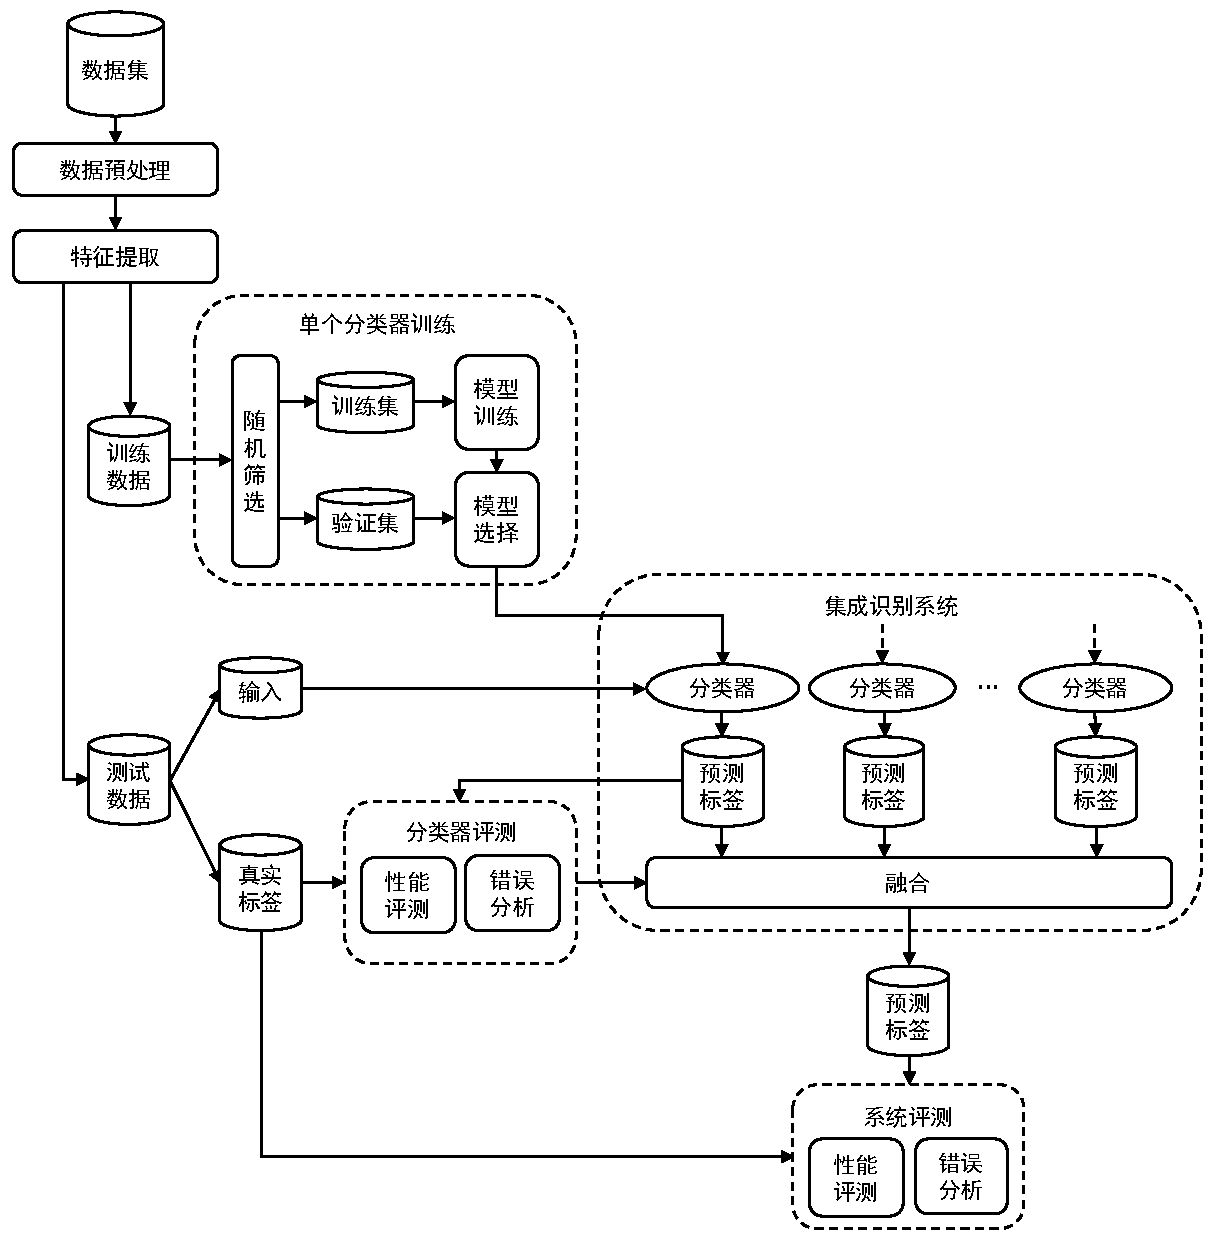
\includegraphics[width=\textwidth]{img/framework.pdf}
  \caption{意图识别的研究框架}
  \label{fig:framework}
\end{figure}

\section{研究框架}
\label{sec:global_framework}

在本小节,我们将根据前述的形式化表示给出一个意图识别的研究框架。由于在本论文的后续研究均面向英语社交媒体文本的分类问题,我们会针对此研究方法对框架进行细化,从原始文本的输入到最终识别目标的输出,理清其中每个步骤的功能和目的,给出一个集成系统的设计框架。针对不同的应用的场景,在后续实验章节中将给出具体的实现方案。

\subsection{框架入口}

图~\ref{fig:framework}显示本文面向意图识别的研究框架。整个框架的输入是实验的数据集,数据集的每个样本包含三个元素,分别是研究的主体、背景信息和意图的倾向。参考前一小节的形式化表示,一个样本可以表示为 $<t, b, c> \in T \times B \times C$。不论是训练数据或测试数据,他们都采用相同的数据预处理技术和特征提取技术来获取样本的特征,以用作分类器的输入,即透过$F_T$和$F_B$分别获取$f_t=F_T(t)$和$f_b=F_B(b)$。

\subsection{基础分类器}

在特征提取完成后,识别模型的输入就准备好了。接下来首先对基础分类器进行研究和分析,比较不同模型和不同参数在对应问题上的整体性能。对于机器学习方法,在模型的训练过程中,需要将训练数据会分成训练集和验证集两个部分。训练集用于调整模型的参数,根据预先设计的损失函数计算模型当前的预测结果和实际标签的偏差,透过微分计算出参数的调整方向,并以一定的学习步长逐步迭代。由于以上训练过程在数学逻辑上是以达到训练集上的最优解来调整参数,会出现对训练样本过拟合的问题,因此会采用验证集来评估模型对训练集以外的样本的识别性能。在每一轮参数调整后计算当前模型在验证集上的性能指标,最后选择其中最优的一轮参数作为该次模型训练最终的参数。

除了分析不同模型在对应问题上的整体性能,透过对被分类器错误识别的样本进行观察,我们需要分析单个分类器的性能局限在哪,分类器对哪些类别的样本有更高的正确率或召回率,哪些样本之间容易出现混淆,或者在输入数据当中是否存在一些有关键信息的特征没有被成功提取。特别地意图识别的研究课题中,我们会关注数据集标签的正确性。在实验的过程中我们假设标签是正确,但有研究指出自动标注会引入噪声\cite{littlestone1988learning},人工标注则难以避免地存在主观性。虽然对不同算法之间的性能比较影响不大,但对于技术水平的评估有其分析的价值。

\subsection{集成识别系统}

经过对基础分类器的分析后,我们对不同模型的识别性能有了深入的了解。为了进一步达到更好的性能,
下一步是基于基础分类器研究集成识别系统的策略和设计。我们提出了一种集成系统的设计方案,结合多个模型相同的分类器的预测结果来作出最终判断,旨在只使用一种模型的基础上尽可能提升识别的性能,或针对特定的性能指标对整个系统的识别倾向进行调整。参考决策树,其识别过程可以认为是一系列的决策,每一步决策都建立在前一步的决策结果上,并且只关注原始问题中的子问题。类似地,我们提出的集成系统经过多次决策来对样本进行意图识别,第一步先由一个分类器或多个分类器的预测结果融合得到一个基础的预测结果,接下来的每一步需要先对前一步的混淆矩阵进行分析,根据哪些类别的样本被误判对指标的影响较大,设定一个子识别任务,从训练数据中筛选出相关的子集来训练新的基础分类器,得出针对该子识别任务的决策结果,决定是否修改上一步中的预测结果。这一方法的原理在于相同的模型在相同配置下的拟合能力是有限的,而子识别任务是原始问题的简化,模型可以专注于拟合一个局部问题,并对前一步的预测结果提出修改意见,起着补丁的作用。具体方法将在后续实验章节中给出详细说明。

同样地,我们需要分析集成系统的性能。在测试数据上,观察系统经过每一轮决策调整之后的识别性能变化,验证系统框架的设计是否满足假设。另外深入观察混淆矩阵的变化,分析各个子识别任务有效的原因,判断其适用和不适用的场景。

\section{本章小结}

在本章我们首先对意图识别给出统一的形式化表示,引出了其中涉及的各个元素并描述他们的相互关系。然后描述了我们面向意图识别的研究框架,其中包括了两个研究重点。一是研究以不同算法得到的分类器对研究问题的整体性能,并作深入的分析,包括单个算法对不同类别样本的识别能力、比较不同算法在不同指标上的区别以理解他们的拟合倾向、观察被错误识别的样本并找出其原因等。二是研究基于基础分类器的集成系统,鉴于单个分类器的识别能力有限,我们提出了一个集成系统的设计方案,旨在结合多个基础分类器的预测结果来得出最终的判断,从而充分发挥一个数学模型的拟合能力,细节实现方法将在后续具体的应用场景中给出说明。




%\chapter{意图识别技术}
\label{cha:tech}

\section{本章引论}

根据前一章中描述的研究框架,在本章中我们将针对每一个功能介绍对应的技术实现,其中包括文本预处理、词特征提取、分类算法、集成学习。对后续实验用中使用到的技术给出相对充分的说明,同时也会相关的技术给出概要的描述,以便于其他研究者在本论文未深入探索的方向作出拓展性的研究。

\section{文本预处理}

文本的预处理是所有面向文本的研究的第一步,其目的是为特征提取做好准备。良好的预处理策略可以在尽可能不掉失重要信息的情况下对样本数据进行简化,增加样本之间重复的模式,减轻模型对数据进行拟合的负担,同时更有效地找出数据之间的相互关系。错误的预处理策略会会掉失具有区分能力的信息,甚至产生具有误导性的样本。对于不同的语言,由于其天然的性质不同,预处理的方法也会各异,以下会重点介绍针对社交媒体上英语文本的预处理技术。

\subsection{分词}

为了从文本提取词级别的特征,我们需要首先将句子切成多个词的序列。

虽然对于英语及大部分欧洲语言,空格隔开的字符必然属于不同的词组,但对于不以空格分隔词组的语言(如中文),分词的作用尤其重要。在某些情况下,分词的结果会影响对句子的理解,如将“乒乓球拍卖完了”切割成“乒乓球拍-卖-完-了”或“乒乓球-拍卖-完-了”,对主体应该是“乒乓球拍”还是“乒乓球”,动词应该是“卖”还是“拍卖”,仅凭字面意思无法确定发言者想表达的意思。特别地社交媒体平台上,新词不断的出现,要正确进行分词就有其独特的难点。而分词并不只针对语言中的单词,还针对标点符号或其他特征字符组成的有特殊语义或情感的字符组合,如现今社交媒体上普遍用多个字符拼接成颜文字,其中最常见的微笑的表情“:)”和伤心的表情“:(”,但如果在分词过程中把前者分割成“:”和“)”就会失去其所带的正向情感信息,这在短文本的情感识别中非常关键。

虽然利用空格和标点符号在大部分情况下可以完成对英语句子的分词,但在一些情况下,标点符号作用为词组的一部分而不是词组的分隔符,而在社交媒体上会有空格被省略的情况,以下是一些需要额外处理的情况\cite{jackson2007natural}\cite{mitkov2004oxford}。一是带句号的缩写,如“U.S.”,“.com”,句号应该作为词的一部分,或按句号切割“U.S.”将失去其语义。二是具有一定格式的带标点符号的词组,如电子邮箱地址(如example@email.com)、时间(如 Jan 6th、06/01/19)、电话号码(如(123)456-7890)、网页地址(如www.example.com)等,而在大部分情况下,我们会优先关注这个字符串指的是什么类型的事物而不是细节,譬如将一个句子中的电子邮箱地址或电话号码作替换并不会改变其情感的表达,但识别出一个字符串对应的事情类型,并在清楚它对意图识别没有关联的情况下对其忽略是有意义的。第三种情况是附属词,如“'t”对应“not”,只有正确识别“'”的作用才能识别出否定的意思,否则句子的意思将完全相反。值得注意的是,对社交媒体平台上的文本,除了以上在正规英语中会出现的情况,还有出现其他特殊情况,如“Y!E!S!”和“N!O!”。这需要对数据首先进行人工观察找出特殊的模式,再对语料库进行统计判断其出现频率,若出现频率较高则新增处理规则将对应模式做转换(如将“Y!E!S!”替换成“YES!!!”)或对问题无关的模式忽略(如国外的微博以“RE:”开头表示回复,并不包含任何情感)。

\subsection{拼写修正}

在处理较正式的文件时,我们一般可以默认其文本满足正规的语言语法,词汇基本都是正确的拼写或故意设计的新词(如杂志专栏作家首创针对英国退出欧盟首创单词“Brexit”)。不过在社交媒体上,拼写不符合传统英语的情况则非常普遍,这些情况可以分成三大类。

第一类是非刻意的拼意错误,由于社交媒体上的文本普遍是非正式的,用户不会刻意去保证文本的语言正确性,他们更关注于表达自己的想法、感情或其他意图。拼写修正技术一般基于统计的方法,对于一个不存在的词汇,尝试对其拼写进行有限次编辑,再评估编辑后的词在其上下文中出现的概率,最后选出可能性最高的一个词作替换。拼写修正技术已相当成熟地被应用于搜索引擎和手机键盘等应用中,读者可参考相关研究\cite{ahmed2009revised}\cite{nejja2015context}了解其细节。

第二种情况是网络上常用的代替用词,如以“thx”、“tnx”代替“thanks”,以“k”代替“ok”,以“cant”代替“can't”。虽然这些用法没有被认可为标准用法,但由于方便而在网络上被传播开成功网民们都能理解的用词。对此应对方法有两种,一是人工建立映射表,把代替用词映射到标准的英语词汇,优点在于可以直接引用标准词汇的语义信息,但缺点是需要人工参与,特别是在网络上新用词不断出现的情况下需要持续的更新。另一种是不做处理,利用机器学习方法从大型语料库中自动学习出它的语义,优点在于省去了人工的部分,缺点在于单词的出现很稀疏,对语料库的依赖很强。

第三种情况是语气加强,如“yeeeees”,“AMAZING”,但对于这一类情况处理的重点不只在于转换成标准用词,而是根据具体的应用问题判断是否要保留这个词存在语气加强的这个信息,譬如在情感识别中,语气加强一般提示了此处的情感需要注意。Baziotis等人\cite{baziotis2017semeval2}的做法是在单词前后添加标签示意,如“yeeeees”替换成“yes <enlongated>”,“AMAZING”替换成“amazing <allcaps>”。

\subsection{规范化}

pass

\section{特征提取}

pass

\subsection{词嵌入}

pass

\subsection{词汇特征} % Lexical Feature 

% 多元语法 n-gram
%   统计数据集中多元语法的词频(TF)和逆文本频率(IDF)
%   取TF-IDF最高的N个多元语法
%   对每个条微博得出一个N维向量, 每一维分别对应一个多元语法,其值为该多元语法在该条微博中的数量乘以该多元语法在整个数据集中的IDF
%   每条微博的向量分别进行归一化
% 单词数量
% 字母数量

\subsection{句法特征} % Syntactic features 

% 对文本中单词转换成词性(Part-of-speech, POS)标注
% 和词汇特征中多元语法一样的计算的TF-IDF特征

\subsection{语义特征} % Semantic features

% 词向量平均和
%   对文本进行分词
%   将单词序列转换成词向量序列
%   取词向量序列的平均和作为特征
% 潜在语义
%   利用潜在语义分析(Latent semantic analysis, LSA)从训练集学习单词间的隐藏概念
%   再分别对测试集各个样本提取隐藏概念
% 词类分布
%   利用布朗聚类(Brown Clustering)对训练集的单词进行聚类(N类)
%   每段文本得出一个N维向量,各维对应该文本中包含该类单词的数量

\subsection{基于人工神经网络}

% 人工神经网络对每一个输入进行预测的中间结果可被认为是该输入的隐藏特征
% 利用不同标注的数据集训练的人工神经网络可以用作对应类型的特征提取,如
%  SemEval2014 Task 9: 标注为文本的正负中性情感
%  SemEval2018 Task 1: 标注为文本中是否分别包含了11种情感


\section{分类算法}

pass

\subsection{传统机器学习方法}

% 支持向量机 Support Vector Machine, SVM
% 决策树 Decision Tree
% 随机森林 Random Forest

\subsection{深度学习方法}

% Gated Recurrent Unit, GRU 
% 长短期记忆网络 Long Short-Term Memory, LSTM
% 双向长短期记忆网络 Bidirectional Long Short-Term Memory, BLSTM
% 卷积神经网络 Convolutional Neural Network CNN

\section{集成学习}

pass

% 后融合
%   结合多个子系统的预测结果,根据特定策略得出新的预测结果

%   多数投票 Majority Voting / Hard Voting
%     每个模型分别给出预测标签
%     取最多模型预测的标签作为最终预测结果

%   加权多数投票 Weighted Majority Vote
%     每个模型分别给出预测标签
%     对这些模型的预测标签进行加权投票,取投票最多的标签作为预测结果

%   加权平均概率投票 Soft Voting
%     每个模型分别给出各个标签的预测概率
%     对每个模型的预测概率进行加权不均,取概率最高的标签作为预测结果


\section{本章小结}

pass

\chapter{面向微博的反讽识别}
\label{cha:exp_irony_det}

\section{本章引论}

社交媒体的发展对我们的语言体系带来了很大的影响,网络上出现了很多新颖的用词和句式,语言的表达方式越来越丰富,也越来越复杂。而反讽是在网络上常见的语言修饰手法之一, 这为反讽相关的研究带来了充足的数据基础。Henry Watson Fowler在《The King's English》一书中指出反讽的使用使得“表面意思和实际意思不同”。譬如一个人说“你这想法真有创意”,在字面意思上是对另一个人的赞同,但在特定背景下,如后接一句“你真相信这能实现吗”,那么发言者实际上可能暗示这个想法无法落地,表面上称赞为“有创意”,其实是指责这种想法不切实际。这在意图识别当中尤其重要,忽略反讽的使用会导致对内容的错误理解,而且这种理解是和真实意思截然相反的,因此识别出反讽的使用或许对相关的场景如情感识别、人机交互能起着正面的作用。

根据Joshi等人\cite{joshi2017automatic}对近年相关研究的总结,反讽识别可以大致分成基于规则的方法和基于机器学习的方法。基于规则的方法透过人工找出反讽中的语言规律,设计出对应的模式,然后在新样本中尝试识别出相应的模式出现。和机器学习方法对比,基于规则的方法优点在于无需模型训练,但要求研究员对反讽有充分的语言理解,设计的模式对样本的复盖程度决定了算法的识别能力。而随着近年深度学习快速发展,一些研究更专注于对词嵌入向量的使用以及人工神经网络的设计和选择。

国际比赛SemEval-2018的任务三\cite{van2018semeval}旨在促进英语微博中的反讽识别研究,其中包含了两个子任务。子任务一是二分类的反讽识别,需要识别微博是否有使用反讽。子任务二是四分类的反讽识别,是子任务一的拓展,除了判断微博是否包含反讽,反讽再细分成三个类别:基于相反语义的反讽 
、情景反讽、其他反讽。本章节中我们将基于SemEval-2018的任务三进行实验,采用比赛组织者提供的训练数据和测试数据,并透过和其他参赛系统进行比较来评估我们提出的框架的性能。

本章的内容安排如下。在章节\ref{sec:exp_irony_det_format}中,我们会基于章节\ref{sec:global_problem_analysis}首先给出当前问题的形式化表示。在章节\ref{sec:exp_irony_det_data}中我们再对具体实验数据进行观察,分析微博文本的特性以及各个反讽类别之间的不同。在章节\ref{sec:exp_irony_det_framework}中,我们会基于章节\ref{sec:global_framework}的框架给出我们对当前问题的系统框架。最后在章节\ref{sec:exp_irony_det_exp}给出实验的细节,以及对实验结果进行分析。

\section{形式化表示}
\label{sec:exp_irony_det_format}

在本章中,我们要研究单条微博的反讽类型识别。给定一个反讽类别集合$C$,对于一个微博集合$T$,对任意一条微博$t \in T$,它属于唯一一种情感类别$c \in C$。又给定一个词集合$W$,微博$t$经过文本预处理后可以表示为一个长度为$L$的词序列 $w = <w_1, w_2, ..., w_L>, w_i \in W, i \in [1, L]$。因为没有引入上下文信息,所以背景$B$在模型中忽略。那么我们的目标是找出一个映射关系$F_C$,使得$c=F_C(w)$。

\section{数据观察}
\label{sec:exp_irony_det_data}

我们的实验完全采用SemEval-2018的任务三比赛组织者提供的数据集,其中的语料收集自微博平台Twitter上发布于2014年至2015年之间的微博,再由人工标注得出每条微博的反讽类型。该比赛的两个子任务均采用了相同的语料但标注稍有不同。子任务一是二分类的反讽识别,需要识别微博是否有使用反讽,各类别的数据分布如表\ref{tab:semeval_2018_task3_A_data}所示,表\ref{tab:semeval_2018_task3_A_sample}为语料中两个类别的例子。可以看出没有反讽和带有反讽两个类别的样本在训练集上大致比例为1:1,在测试集上两个类别的分布大致为3:2。

\begin{table}[htb]
  \centering
  \begin{minipage}[t]{0.7\linewidth} % 如果想在表格中使用脚注,minipage是个不错的办法
  \caption{反讽识别子任务一各类别样本数量分布}
  \label{tab:semeval_2018_task3_A_data}
    \begin{tabularx}{\linewidth}{X|XX}
    \toprule[1.5pt]
    数据集 & 没有反讽 & 带有反讽 \\  
    \hline
    训练集 & 1923 & 1911 \\
    测试集 & 473  & 311 \\
    \bottomrule[1.5pt]
    \end{tabularx}
  \end{minipage}
\end{table}

\begin{table}[htb]
  \centering
  \begin{minipage}[t]{0.8\linewidth} % 如果想在表格中使用脚注,minipage是个不错的办法
  \caption{反讽识别子任务一样例}
  \label{tab:semeval_2018_task3_A_sample}
  \begin{tabularx}{\linewidth}{l|X}
    \toprule[1.5pt]
    反讽类别 & 例子 \\
    \hline
    没有反讽 & Had no sleep and have got school now \#not happy \\
    带有反讽 & I just love when you test my patience!! \#not \\
    \bottomrule[1.5pt]
  \end{tabularx}
  \end{minipage}
\end{table}

子任务二是四分类的反讽识别,是子任务一的拓展,除了判断微博是否包含反讽,反讽再细分成三个类别:基于相反语义的反讽、情景反讽、其他反讽。各类别的数据分布如表\ref{tab:semeval_2018_task3_B_data}所示,表\ref{tab:semeval_2018_task3_B_sample}为语料中各反讽类别的例子。可以看出带有反讽一类细分成三个子反讽类别后各个类别的分别变得明显的不均匀,三个子反讽类别中的样本数据量差异也较大,基于相反语义的言语反讽占了其中一半以上,在模型训练过程应有对应策略处理。

\begin{table}[htb]
  \centering
  \begin{minipage}[t]{\linewidth} % 如果想在表格中使用脚注,minipage是个不错的办法
  \caption{反讽识别子任务二各类别样本数量分布}
  \label{tab:semeval_2018_task3_B_data}
    \begin{tabularx}{\linewidth}{X|XXXX}
    \toprule[1.5pt]
    数据集 & 没有反讽 & 基于相反语义的反讽 & 情景反讽 & 其他反讽\\  
    \hline
    训练集 & 1923 & 1390 & 316  & 205 \\
    测试集 & 473  & 164  & 85  & 62 \\
    \bottomrule[1.5pt]
    \end{tabularx}
  \end{minipage}
\end{table}

\begin{table}[htb]
  \centering
  \begin{minipage}[t]{\linewidth} % 如果想在表格中使用脚注,minipage是个不错的办法
  \caption{反讽识别子任务二样例}
  \label{tab:semeval_2018_task3_B_sample}
  \begin{tabularx}{\linewidth}{l|X}
    \toprule[1.5pt]
    \small 反讽类别 & 例子 \\
    \hline
    \small 没有反讽 & Had no sleep and have got school now \#not happy \\
    \small 基于相反语义的反讽 & \small I really love this year’s summer; weeks and weeks of awful weather \\
    \small 情景反讽 & Most of us didn’t focus in the \#ADHD lecture. \#irony \\
    \small 其他反讽 & @someuser Yeah keeping cricket clean, that's what he wants \#Sarcasm \\
    \bottomrule[1.5pt]
  \end{tabularx}
  \end{minipage}
\end{table}

比赛组织者对四种反讽类别给出了对应的说明。对基于相反语义的反讽一类,文本中存在某部分内容表达了可评估的情感极性,但整条微博实际上表达了相反的情感极性。如表\ref{tab:semeval_2018_task3_B_sample}中的例子,“love”在字面意思上表达了正面的情感,但微博后半中“awful weather”提示实际情况引起了发言者的不适,发言者其实在表达对这个夏天坏天气的不满,这和“love”的正面情感恰恰相反。对于情景反讽一类,文本正描述某个场景,其中发生的事情和某种预期不符。如表\ref{tab:semeval_2018_task3_B_sample}中的例子,描述了一个参与讲座的场景,但“我们(us)”并没有专注于这场讲座,和“参与者应该专注于讲座内容”的预期相反。对于其他反讽一类,文本表达了讽刺的意思,但文本的字面意思和发言者表达的意思之间并不存在情感极性的反差。如表\ref{tab:semeval_2018_task3_B_sample}中的例子,发言者表示某人想要保持蟋蟀干净,字面上并不存在情感极性,但在句子后的井号标签提示了发言者表达了讽刺,认为“保持蟋蟀干净”是一样莫名奇妙的事情。最后是没有反讽一类,对于明显不可能包含反讽的文本,或者在背景信息不足的情况下不能确认其包含反讽的文本均属于这一类。

\subsection{文本长度}

我们首先对数据集的文本经过简单分词后统计各个类别的样本中词数量的分布,以下简称为文本长度。表\ref{fig:semeval2018_task3_train_class_len}和表\ref{fig:semeval2018_task3_test_class_len}分别显示了训练集和测试集上各类别样本的文本长度。综合先见样本的文本长度不超过了50,样本的平均文本长度约为20个词。根据表\ref{fig:semeval2018_task3_train_class_len}我们可以看出“情景反讽”的样本整体的文本长度较其他类别的长,“没有反讽”和“基于相反语义的反讽”在文本长度分布上没有明显区别,“其他反讽”整体的文本长度则略高于前两者。再观察表\ref{fig:semeval2018_task3_test_class_len},同样地“没有反讽”和“基于相反语义的反讽”在文本长度分布上没有明显区别,“情景反讽”的文本长度略高于前两者,但不如训练集上明显。

\begin{figure}[H]
  \centering
  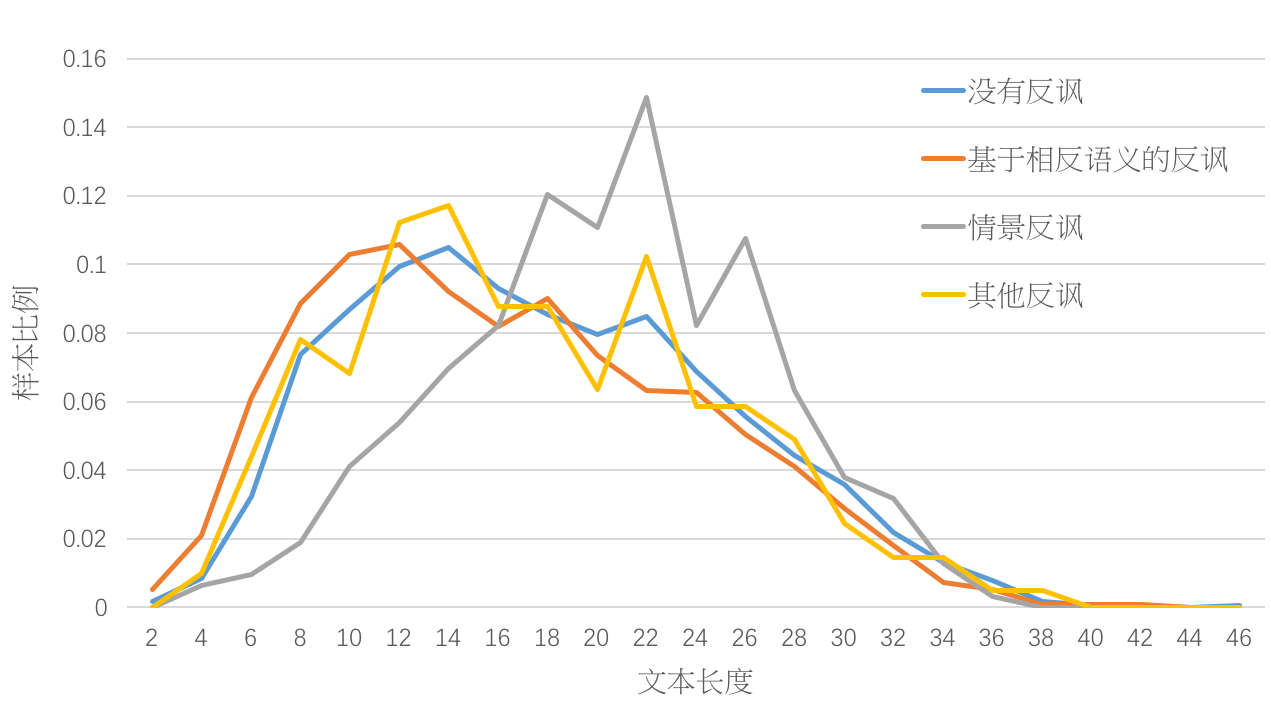
\includegraphics[width=\textwidth]{img/semeval2018_task3_train_class_len.png}
  \caption{反讽识别训练集上各类别文本长度分布}
  \label{fig:semeval2018_task3_train_class_len}
\end{figure}

\begin{figure}[H]
  \centering
  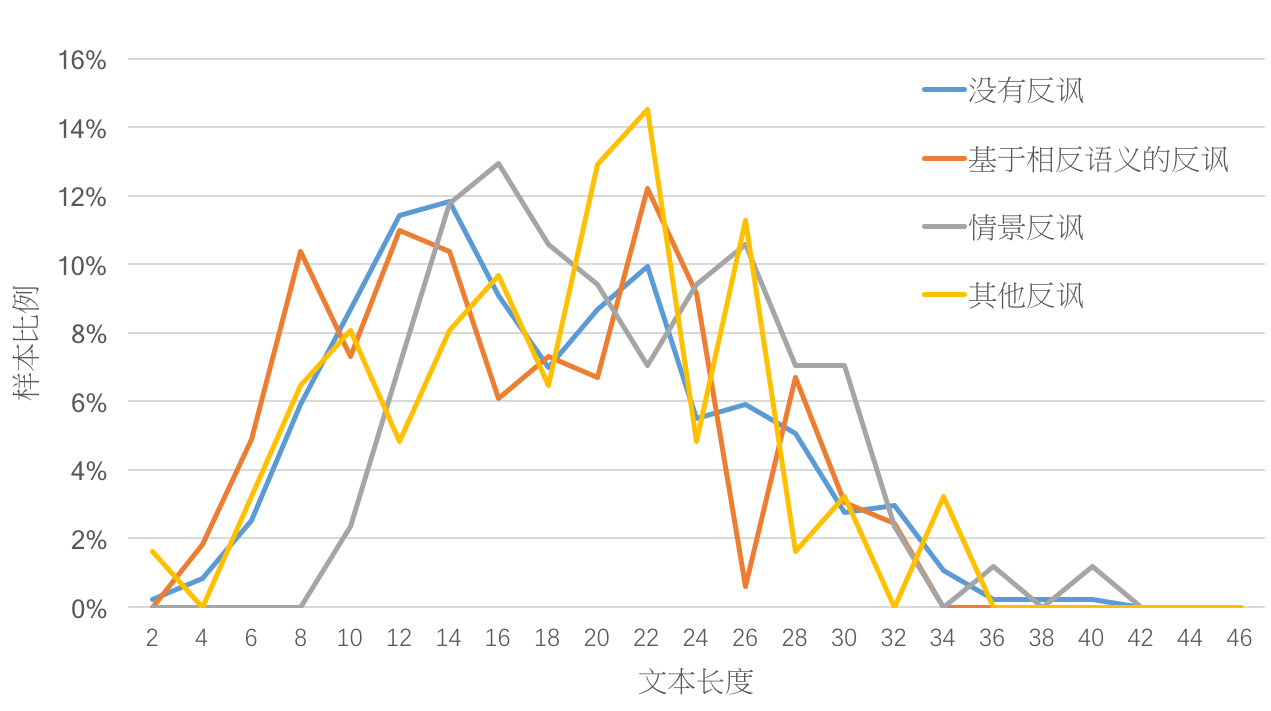
\includegraphics[width=\textwidth]{img/semeval2018_task3_test_class_len.png}
  \caption{反讽识别测试集上各类别文本长度分布}
  \label{fig:semeval2018_task3_test_class_len}
\end{figure}

\subsection{文本特征}
\label{ssec:exp_irony_det_data_text}

另外我们注意到语料中存在微博平台Twitter上特有的文本特征,出现频率较高的模式如下:

\begin{itemize}

\item 用户标签“@someuser”,对应微博上的一个用户,使用场景包括以下两种。一是作为句子中的名词使用,二是添加在句前或句末用于提示该用户的参与,不具有句法作用。

\item 井号标签“\#something”,使用场景大致分为以下两种。一是作为句子中的一部分,如“I \#do \#like \#it”,去除井号后满足正规的英语用法,此处以井号标签代替是对内容的强调。另一种是出现在句末,用于提示微博内容与标签对应内容相关,如句末出现“\#sarcasmtweet”明显表示讽刺。

\item 网站链接,在微博平台上支持附加一个网站链接以便,其中平台对链接进行了统一处理,在语料库中网站链接均形如“http://t.co/***”或“https://t.co/***”。

\item 转发标记“RT”(retweet),当用户转发某条微博并添加个人评论时,平台会自动在个人评论后附加转发的微博原文并以“RT”隔开。

\item 一些在社交媒体平台上常见的、有别于正规英语的用法,如拼写错误、缩略词、全大写字母的单词、表情符等,可以参考章节\ref{sec:text_preprocess}描述的例子。

\end{itemize}


\section{框架设计}
\label{sec:exp_irony_det_framework}

对于任务一,由于是二分类问题,我们的系统只包含一组二分类器,透过一次投票得出最终的预测结果,判断微博文本是否采用了反讽修辞。

对于任务二,我们提出的识别系统包含了四组分类器,分别面向不同的子分类问题,并依次经过四次投票结合各组分类器的预测结果来得出最终的预测结果。第一组分类器由$N_1$个四类分类器组成,对应原问题的四个类别。第二组分类器由$N_2$个二类分类器组成,用于区分“没有反讽”和“基于相反语义的反讽”两类。第三组分类器由$N_3$个二类分类器组成,用于区分“没有反讽”和“情景反讽”两类。第四组分类器由$N_4$个二类分类器组成,用于区分“没有反讽”和“其他反讽”两类。

对于一条待识别的微博,决策过程如下:

\begin{itemize}

\item 首先由第一组分类器内部进行多数投票得出$Label^{1}_{MV}$作为第一轮预测结果$Label_{I}$ 。为方便阅读,以下将对一组样本的第一轮预测结果称为中间结果一。

\item 第二步,由第二组分类器投票进行多数投票得出预测结果$Label^{2}_{MV}$,若超过$thr_{2}$分类器投票投给$Label^{2}_{MV}$且第一轮的预测结果$Label_{I}$为“没有反讽”或“基于相反语义的反讽”,则把预测结果修改为$Label^{2}_{MV}$,否则保持不变,以此得出第二轮的预测结果$Label_{II}$。为方便阅读,以下将对一组样本的第二轮预测结果称为中间结果二。

\item 第三步,由第三组分类器投票进行多数投票得出预测结果$Label^{3}_{MV}$,若超过$thr_{3}$分类器投票投给$Label^{3}_{MV}$且第二轮的预测结果$Label_{II}$为“没有反讽”或“情景反讽”,则把预测结果修改为$Label^{3}_{MV}$,否则保持不变,以此得出第三轮的预测结果$Label_{III}$。为方便阅读,以下将对一组样本的第三轮预测结果称为中间结果III。

\item 最后一步,由第四组分类器投票进行多数投票得出预测结果$Label^{4}_{MV}$,若超过$thr_{4}$分类器投票投给$Label^{4}_{MV}$且第三轮的预测结果$Label_{III}$为“没有反讽”或“其他反讽”,则把预测结果修改为$Label^{4}_{MV}$,否则保持不变,以此得出第四轮的预测结果$Label_{IV}$,同时作为整个系统对该微博的最终反讽识别结果。

\end{itemize}

整个决策过程可以分成两大部分。第一部分是初步完成对微博的四分类反讽识别,作为后续决策的基础,对应上述四步决策中的第一步。第二部分是基于第一部分的初步识别结果进行修正,对应上述四步决策中的后三步,每一步只关注被识别的两个类别的样本,由一组专门的子分类器重新给出识别结果,当新的结果充分可信则修改前一步得到的预测结果。在这里决策的可信度由投票数决定,当多数票由超过$thr$个分类器给出则认为充分可信。

\begin{figure}[H]
  \centering
  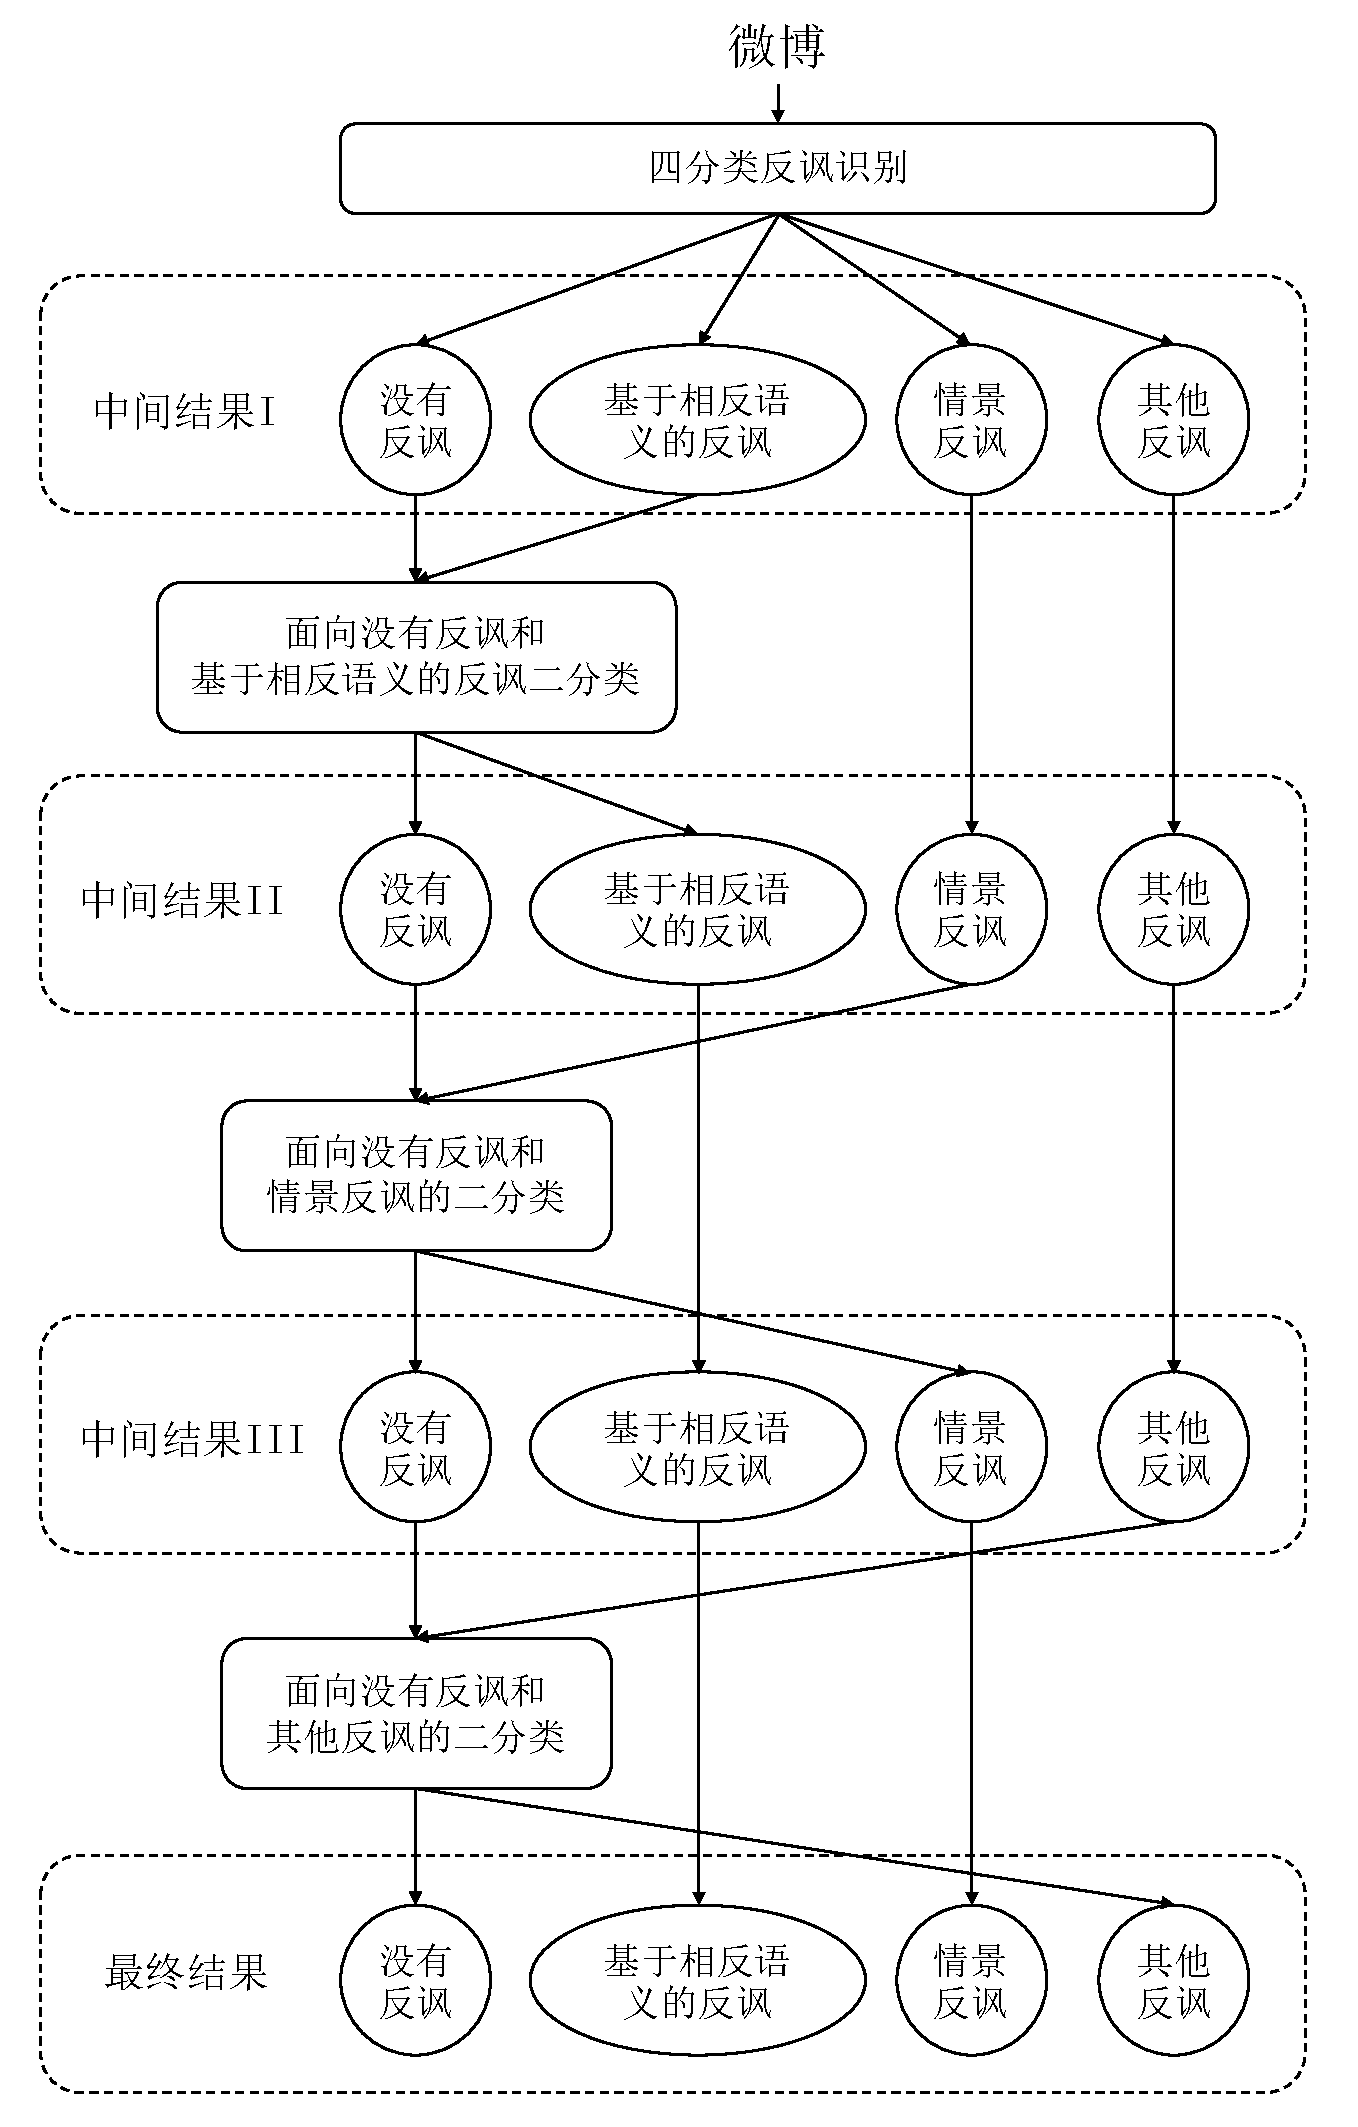
\includegraphics[width=0.9\textwidth]{img/irony_det_system.pdf}
  \caption{面向四分类反讽识别的系统框架}
  \label{fig:irony_det_system}
\end{figure}

其中对于每个子分类问题,我们都采用了相同的模型框架,如图\ref{fig:irony_det_cls_framework}所示,每个子分类器的输入都是微博文本经过预处理后得到的词序列$\{w_i\}$,然后每个词替换成对应的词嵌入向量,作为特征编码器的输入。特征编码器的目的是把微博文本对应的词向量序列转换成固定长度的特征向量,作为其反讽属性相关的表示向量,首先由一层或多层卷积神经网络或迭归神经网络组成,由于一维神经网络和迭归神经网络的输出均为和输入序列等同长度的向量序列,故最后需要再经过一层处理,对于迭归神经网络一般研究会取序列的最后一个向量,在理论上它结合了整段内容的信息,而对于迭归神经网络一般会采到最大池化层,分别取各特征位上的最大值,最后一种是采用注意力机制,对两类神经网络的序列输出均可结合成定长的表示向量。得到的表示向量作为后面概率预测器的输入,概率预测器的目的是基于微博定长的表示向量得出该微博属于各个反讽类别的概率分布,此处统一采用单层的全联接层和$Softmax$作为激活函数。最后取概率最高者作为分类器对该条微博预测的反讽类别。

考虑到对于不同反讽类型,其文本特征的提取方式可能有所不同,不同模型在各个子分类问题上的建模能力和识别性能也因此不同,所以对于每个子分类问题,我们会分别比较各组模型和参数的性能,以求在子分类问题上达到尽可能好的效果。

\begin{figure}[H]
  \centering
  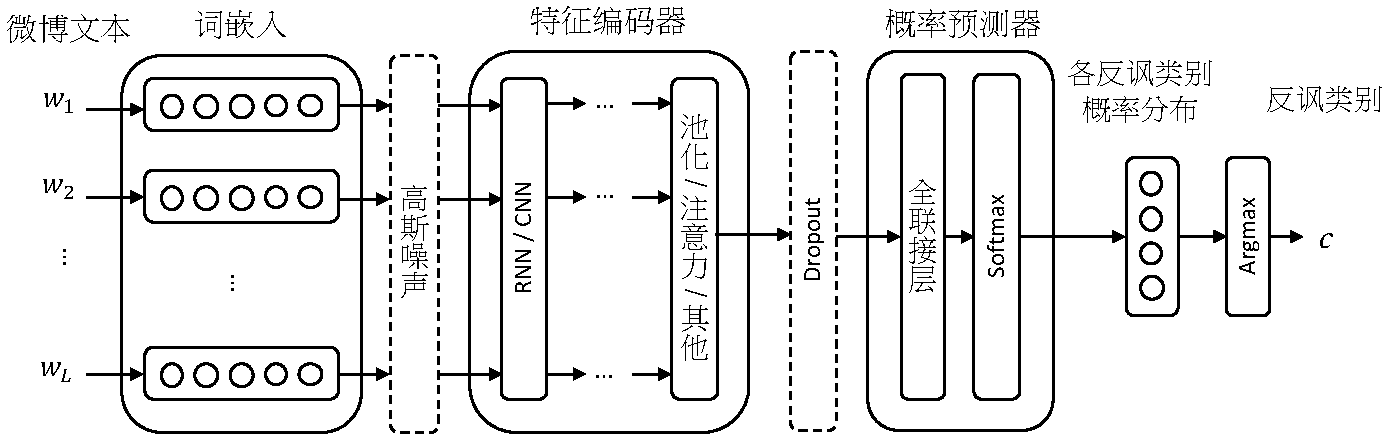
\includegraphics[width=\textwidth]{img/irony_det_cls_framework.pdf}
  \caption{反讽识别子分类器模型框架}
  \label{fig:irony_det_cls_framework}
\end{figure}

\section{实验与分析}
\label{sec:exp_irony_det_exp}

\subsection{数据预处理}

基于我们在章节\ref{ssec:exp_irony_det_data_text}中对样本文本的观察,我们依次采取了以下数据预处理手法

\begin{itemize}

\item 对于不用的用户标签“@someuser”,我们假设具体的用户名不影响微博内容的反讽类型,故统一替换成“<user>”。

\item 对于井号标签“\#something”,我们将他替换成一个字符串序列“<hashtag>”,“something”,“</hashtag>”,此处“<hashtag>”表示井号标签的开始,“</hashtag>”表示井号标签的结束,原因在于在Twitter平台上,井号标签可能由多个单词组成,如语料中出现的井号标签"\#SoCute",其内容应
砌解成“so”、“cute”两个单词,而语料中多单词组成的井号标签普遍以单词首字母大写示意,故可以简单完成分词,同时在前后添加“<hashtag>”和“</hashtag>”示意中间的内容属于同一个井号标签。

\item 全字母大写的内容在前后添加“<allcap>”和“</allcap>”,示意这一段文本可能是用户故意表示强调的内容。

\item 重复大于等次三次的标点符号以“<repeated>”示意,如“!!!”替换成序列“!”和“<repeated>”,表示“!”被多次重复以表达语气加强,同时假设重复次数不影响反讽的类型。

\item 将字母被故意重复的单词以“<elongated>”示意,如“Noooooooo”替换成序列“No”和“<elongated>”,表示“No”中某一个或多个字母被多次重复,但假设被重复的字符和重复的次数与反讽类型无关。

\item 将数字串替换成“<num>”,将电话号码替换成“<phone>”,将日期和时间分别替换成“<date>”和“<time>”,将数字百分比替换成“<percentage>”,超链接替换成“<url>”

\item 将由多个标点符号组成的表情符替换成对应的情感标签,如将“:)”替换成“<happy>”,将“:((”替换成“<sad>”。

\item 在完成以上处理后,对英文的大小写统一转换成小写。

\end{itemize}

以上功能我们利用了第三方的英语微博文本处理工具\textit{ekphrasis}\footnote{https://github.com/cbaziotis/ekphrasis}完成,对于其中如何分词、如何识别电话号码和日期、以及颜文字到情感标签的详细映射关系列表,读者可以直接参考其代码实现和配置文件。

\subsection{实验设置}

以下实验主要分成两大部分。第一部分是分析不同模型在不同子分类问题下的性能,根据章节\ref{sec:exp_irony_det_framework},我们最终的反讽识别框架涉及以下多个子分类问题:区分四个反讽类别的四分类问题、区分“没有反讽”和“基于相反语义的反讽”的二分类问题、区分“没有反讽”和“情景反讽”的二分类问题、区分“没有反讽”和“其他反讽”的二分类问题。对于各个子分类问题,我们基于章节~\ref{sec:exp_irony_det_framework}中的子分类模型框架进行实验,透过采用不同配置了解不同模型文本反讽识别的拟合能力。

第二部分是分析我们设计的识别系统的性能。我们会观察每一轮决策的调整如何改变局部的预测结果,而这些局部变化如何影响系统的整体性能。

%另外我们也会透过对设计的系统框架进行修改和比较,分析设计的合理性,以及当尝试将这种识别系统设计方式应用到其他场景时有哪些细节值得注意。

\subsection{评价指标}

按照国际比赛SemEval-2018任务三的设置,各个任务均以F1值作为识别系统性能的主要评价指标。对于其中一个类别$c$的F1值,其定义如下:

\begin{align}
  F_c = \frac{2 \times P_c \times R_c}{P_c + R_c} 
\end{align}

其中 $P_c$ 为类别$c$的正确率,$R_c$ 为类别$c$的召回率,其定义如下:

\begin{align}
  P_c &= \frac{TP_c}{TP_c + FP_c} \\
  R_c &= \frac{TP_c}{TP_c + FN_c}
\end{align} 

其中$TP_c$表示被系统预测为类别$c$,且真实标签为类别$c$的样本数量;$FP_c$表示被系统预测为类别$c$,但真实标签不是类别$c$的样本数量;$FN_c$被系统预测为不是类别$c$,但真实标签为类别$c$的样本数量。对于子任务一,系统性能以“带有反讽”一类样本的F1值为主要评估指标。对于子任务二,系统性能以各个类别的F1值的宏平均作为主要评价指标,即:

\begin{align}
  F1-macro = \sum\limits_{c \in C}F_c
\end{align}

此处$C$对应子任务二中四个类别组成的集合,即\{没有反讽,基于相反语义的反讽,情景反讽,其他反讽\}。在以下实验中,我们除了观察F1值、正确率和召回率,我们还会给出模型的准确率,其定义如下:

\begin{align}
  Acc &= \frac{\sum\limits_{c \in C} TP_c}{\sum\limits_{c \in C}(TP_c + FP_c)}
\end{align}

其中$TP_c$和$FP_c$如前述的定义,而$C$在子任务一中对应两个类别组成的集合,即\{没有反讽,带有反讽\}。

\subsection{模型训练}
\label{ssec:exp_irony_det_model_training}

对于不同的模型,我们都采用了以下策略来进行训练:

\begin{itemize}

\item 对于每个子分类器,在训练开始前我们先从每一类的训练样本中随机选出10\%的样本作为验证集,以此保留各个类的样本量分布。在每一轮模型训练中,学习算法基于另外90\%的训练样本对网络参数进行调整,然后计算模型在验证集上的F1值,经过有限轮迭代后,取在验证集上达到最优F1值的网络参数作为该子分类器最终的参数,以此缓解在训练数据上过拟合的问题。另外由于最终预测结合由多个子分类器投票联合得出,为了充分运用训练数据,每个分类器的验证集为独立随机筛选得出,一方面保证每个训练样本都有概率被用于某个分类器的参数调整,另一方面使得各个分类器的训练数据不同,因此对文本特征的建模也会有所不同,理论上对过拟合同样有缓解的作用,更有利于最后的投票。

\item 对于词嵌入层,我们利用了章节\ref{ssec:embedding}中提到的Baziotis等人\cite{baziotis2018ntua}提供的词嵌入模型,直接用于初始化词嵌入层的参数。在训练过程中,我们不对词嵌入层的参数进行调整。考虑到若允许词嵌入层的参数调整,那么只有在训练集中出现过的词的词向量有机会被修改,词嵌入空间因此有所改动,只出现在验证集或测试集上的词的词向量在新的词嵌入空间中表达的意义就有可能出现偏差。另外对于词嵌入模型中未被覆盖的单词,若它在至少2个训练样本中出现,则为其随机生成词向量。

\item 在训练阶段中,我们在词嵌入层后添加高斯噪音。由于词嵌入算法在原理上使得意思相似的单词投影到词嵌入空间中距离相近的点上,高斯噪音的添加相当于把原本的单词替换成近义词,使得模型能更好地识别近义词构成的语言模式,另一方面缓解过拟合的问题。在验证和测试阶段,高斯躁音的标准方差被调整为零,即不起作用。

\item 在训练阶段中,我们在特征编码器和概率预测器之间添加了Dropout层,以概率$p_{Dropout}$将特征编码器得出特征向量上的各位数值置为零,并对没有被置零的各位数值乘以常量 $\frac{1}{1-p_{dropout}}$。在验证和测试阶段,Dropout层不起作用。

\item 在模型训练的损失函数,我们以权重$l_2$加入了概率预测器中全联接层的权重(不包括偏移量)的L2正则项。

\item 在面向“没有反讽”和“其他反讽”的二分类问题中,由于两个类别的样本数据差异较大(1923:205),当人工神经网络根据样本的误差透过反向传播进行学习时,如果所有样本的权重相同,模型会倾向于把所有样本判断为样本量够多的“没有反讽”。为此我们根据样本量的分布决定各个类别的样本的权重。如公式\ref{eq:class_weight}所示,其中$w_c$表示类别$c$对应每个样本的权重,$N$表示总的训练样本数,$C$表示该子分类问题的类别集合,此处即为\{没有反讽,其他反讽\},$N_c$示类别$c$对应的训练样本数。

\end{itemize}

\begin{align}
    \label{eq:class_weight}
    w_c = \frac{N}{|C| \times N_c}
\end{align}

\subsection{结果与分析}

\subsubsection{面向“带有反讽”和“带有反讽”的二分类模型性能分析}
\label{sssec:exp_irony_det_A_base}

对面向“带有反讽”和“带有反讽”的二分类问题,表~\ref{tab:exp_irony_det_A_single_result}和图~\ref{fig:exp_irony_det_A_single_result_bar}显示不同卷积神经网络和迭归神经网络在测试集上能达到的性能。注意表中的正确率、召回率、F1值均是针对类别“带有反讽”的指标,对应比赛SemEval2018任务三子任务一关注的主要指标。

对于F1值,2层BiLSTM的表现最好,其次是LSTM配合注意力机制,其F1值和前者非常靠近(偏差约0.001),第三为单层的BiLSTM,其F1值和前两者则差距明显(约0.01)。对于准确率,单层BiLSTM配合注意力机制和2层BiLSTM配合注意力机制达到最好的数值0.6888 ,第三为LSTM配合注意力机制,其准确率和前两者偏差较小(约0.026)。对于正确率,2层BiLSTM配合注意力机制达到最好的数值0.5870 ,其次是单层BiLSTM配合注意力机制,与前者偏差较小(约0.001),第三的LSTM配合注意力机制则和和前两者则差距明显(约0.01)。对于召回率,单层的LSTM达到最好的0.8617 ,第二的2层BiLSTM和前者的差距明显(约0.04)。

对于单层BiLSTM和2层BiLSTM,添加注意力机制都使得准确率和“带有反讽”的正确率有所提升,但同时“带有反讽”的召回率明显下降,导致“带有反讽”的F1值也连带下降,可见BiLSTM和2层BiLSTM添加注意力机制后整个模型的拟合能力是有上升的,但更倾向于预测样本为“没有反讽”,导致“带有反讽”的召回率下降,相对地更少比例的样本被误判为“带有反讽”,因而正确率稍为提高。另外CNN在添加注意力机制后,除召回率以外的三项指标都达到了各个模型中最差的性能,可见虽然在公式上注意力机制可以配合CNN使用,但实际性能并不理想。

\begin{table}[htb]
  \centering
  \begin{minipage}[t]{\linewidth}
  \caption{面向“带有反讽”和“带有反讽”的二分类模型性能}
  \label{tab:exp_irony_det_A_single_result}
    \begin{tabularx}{\linewidth}{X|llll}
    \toprule[1.5pt]
    & 准确率 & 正确率 & 召回率 & F1值 \\
    \hline
    CNN & 0.6658 (6) & 0.5548 (6) & 0.7974 (5) & 0.6544 (5) \\ % A_cnn_ek_1553221371
    CNN+注意力机制 & 0.6008 (12) & 0.4980 (12) & 0.8039 (3) & 0.6150 (12) \\  % A_cnn_ek_1554345958
    \hline
    GRU & 0.6607 (7) & 0.5542 (7) & 0.7395 (9) & 0.6336 (10) \\ % A_gru_ek_1553070254
    GRU+注意力机制 & 0.6569 (10) & 0.5482 (9) & 0.7685 (7) & 0.6399 (9) \\ % A_gru_ek_1553074900
    \hline
    BiGRU & 0.6594 (8) & 0.5534 (8) & 0.7331 (10) & 0.6307 (11) \\ % A_bgru_ek_1553075855
    BiGRU+注意力机制 & 0.6582 (9) & 0.5473 (10) & 0.8006 (4) & 0.6501 (7) \\ % A_bgru_ek_1553068355
    \hline
    LSTM & 0.6390 (11) & 0.5276 (11) & \bf 0.8617 (1) & 0.6545 (4) \\ % A_lstm_ek_1553071939
    LSTM+注意力机制 & 0.6862 (3) & 0.5768 (3) & 0.7846 (6) & 0.6640 (2) \\ % A_lstm_ek_1553075765
    \hline
    BiLSTM & 0.6798 (4) & 0.5721 (4) & 0.7653 (8) & 0.6547 (3) \\ % A_blstm_ek_1553075473
    BiLSTM+注意力机制 & \bf 0.6888 (1) & 0.5861 (2) & 0.7331 (10) & 0.6514 (6) \\ % A_blstm_ek_1553583756
    \hline
    2层BiLSTM & 0.6709 (5) & 0.5577 (5) & 0.8232 (2) & \bf 0.6649 (1) \\ % A_nblstm_ek_1554346535
    2层BiLSTM+注意力机制 & \bf 0.6888 (1) & \bf 0.5870 (1) & 0.7267 (12) & 0.6494 (8) \\ % A_nblstm_ek_1554346515
    \bottomrule[1.5pt]
    \end{tabularx}
  \end{minipage}
\end{table}

\begin{figure}[H]
  \centering
  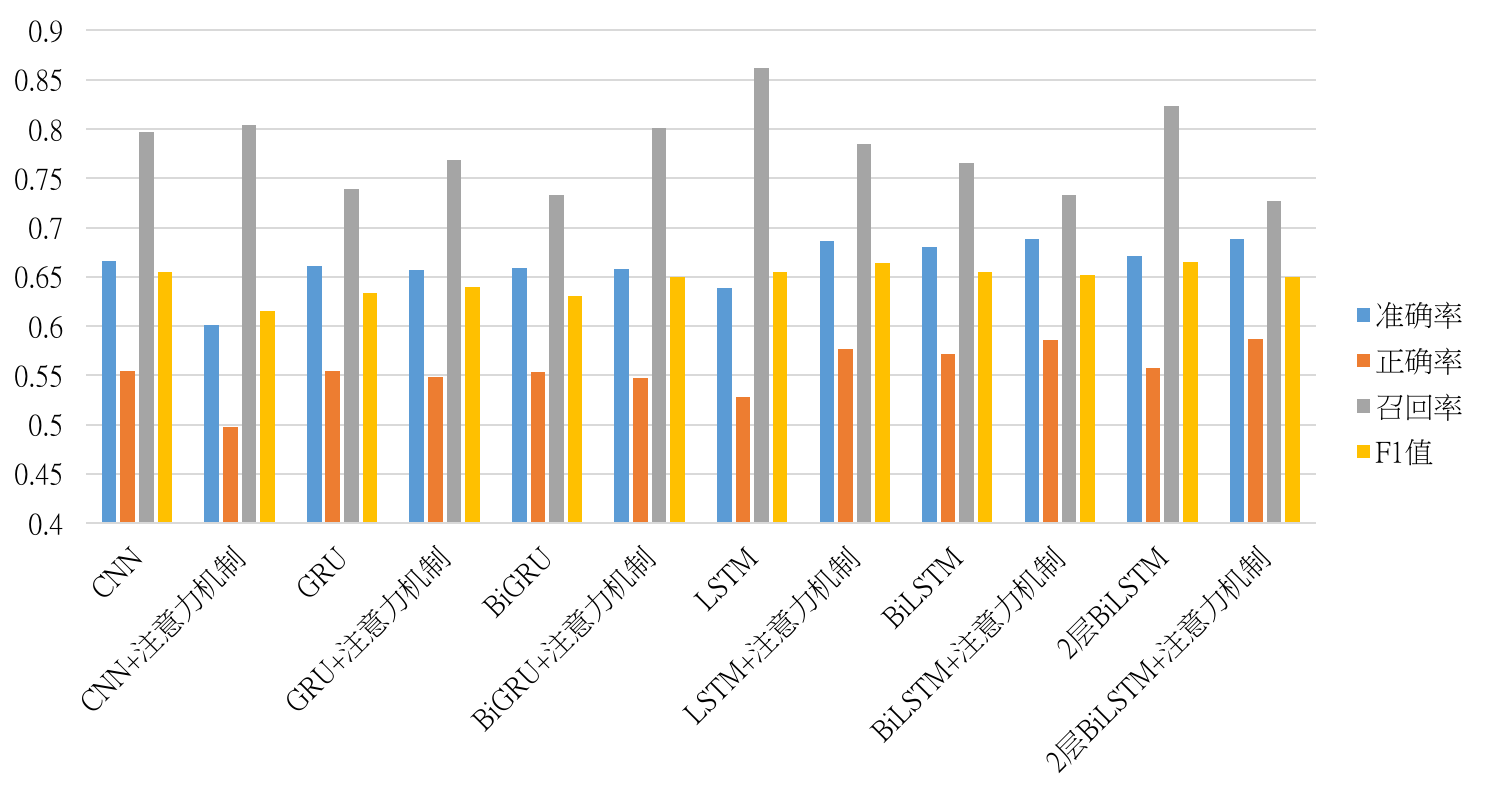
\includegraphics[width=\textwidth]{img/exp_irony_det_A_single_result_bar.png}
  \caption{面向“带有反讽”和“带有反讽”的二分类模型性能}
  \label{fig:exp_irony_det_A_single_result_bar}
\end{figure}

\subsubsection{面向反讽四分类的模型性能分析}
\label{sssec:exp_irony_det_B_base}

对于面向反讽四分类问题,表~\ref{tab:exp_irony_det_B_result}和图~\ref{fig:exp_irony_det_B_single_result_bar}显示不同卷积神经网络和迭归神经网络在测试集上能达到的性能。注意表中的正确率、召回率、F1值均是
各类别对应指标数据的宏平均,对应比赛SemEval2018任务三子任务二关注的主要指标。

对于F1值,BiGRU达到最好的数值(0.4768),其次是2层BiLSTM以及配合注意力机制的2层BiLSTM,与前者的数值差距明显(约为0.01)。对于准确率,同样由BiGRU达到最好的数值(0.6722),其次是BiLSTM和2层BiLSTM,和前者的数值差距明显(约0.014)。对于正确率,CNN和2层BiLSTM的性能较好(在0.5以上),第三的BiLSTM则在0.49以下。对于召回率,2层BiLSTM配合注意力机制达到最好的0.4864 ,其次的BiGRU和BiLSTM则和前者差距明显(约0.01)。

另外,六组模型在添加注意力机制后正确率、召回率和F1值都有所下降(仅2层BiLSTM的召回率例外),而对于准确率较高的BiGRU、BiLSTM和CNN在添加注意力机制后准确率同样有所下降,可以认为添加注意力机制在此子分类问题中并不没有带来性能提升。

\begin{table}[htb]
  \centering
  \begin{minipage}[t]{\linewidth}
  \caption{面向反讽四分类的模型性能}
  \label{tab:exp_irony_det_B_result}
    \begin{tabularx}{\linewidth}{X|llll}
    \toprule[1.5pt]
    & 准确率 & 正确率 & 召回率 & F1值 \\
    \hline
    CNN & 0.6531 (4) & \bf 0.5090 (1) & 0.4667 (5) & 0.4432 (7) \\ % B_cnn_ek_1554446864
    CNN+注意力机制 & 0.6186 (10) & 0.4467 (7) & 0.4214 (12) & 0.4030 (12) \\ % B_cnn_ek_1554446879
    \hline
    GRU & 0.6148 (12) & 0.4437 (8) & 0.4693 (4) & 0.4476 (5) \\ % B_gru_ek_1554447274
    GRU+注意力机制 & 0.6531 (4) & 0.4253 (10) & 0.4605 (7) & 0.4370 (8) \\ % B_gru_ek_1554447525
    \hline
    BiGRU & \bf 0.6722 (1) & 0.4868 (4) & 0.4779 (2) & \bf 0.4768 (1) \\ % B_bgru_ek_1554447516
    BiGRU+注意力机制 & 0.6301 (9) & 0.4543 (6) & 0.4638 (6) & 0.4497 (4) \\ % B_bgru_ek_1554447697
    \hline
    LSTM & 0.6186 (10) & 0.4313 (9) & 0.4490 (9) & 0.4307 (9) \\ % B_lstm_ek_1554447721
    LSTM+注意力机制 & 0.6416 (6) & 0.4046 (12) & 0.4394 (10) & 0.4148 (11) \\ % B_lstm_ek_1554447878
    \hline
    BiLSTM & 0.6582 (2) & 0.4875 (3) & 0.4537 (8) & 0.4447 (6) \\ % B_blstm_ek_1554447955
    BiLSTM+注意力机制 & 0.6352 (7) & 0.4168 (11) & 0.4386 (11) & 0.4160 (10) \\ % B_blstm_ek_1554448216
    \hline
    2层BiLSTM & 0.6582 (2) & 0.5068 (2) & 0.4762 (3) & 0.4644 (3) \\ % B_nblstm_ek_1554448237
    2层BiLSTM+注意力机制 & 0.6314 (8) & 0.4824 (5) & \bf 0.4864 (1) & 0.4657 (2) \\ % B_nblstm_ek_1554448594
    \bottomrule[1.5pt]
    \end{tabularx}
  \end{minipage}
\end{table}

\begin{figure}[H]
  \centering
  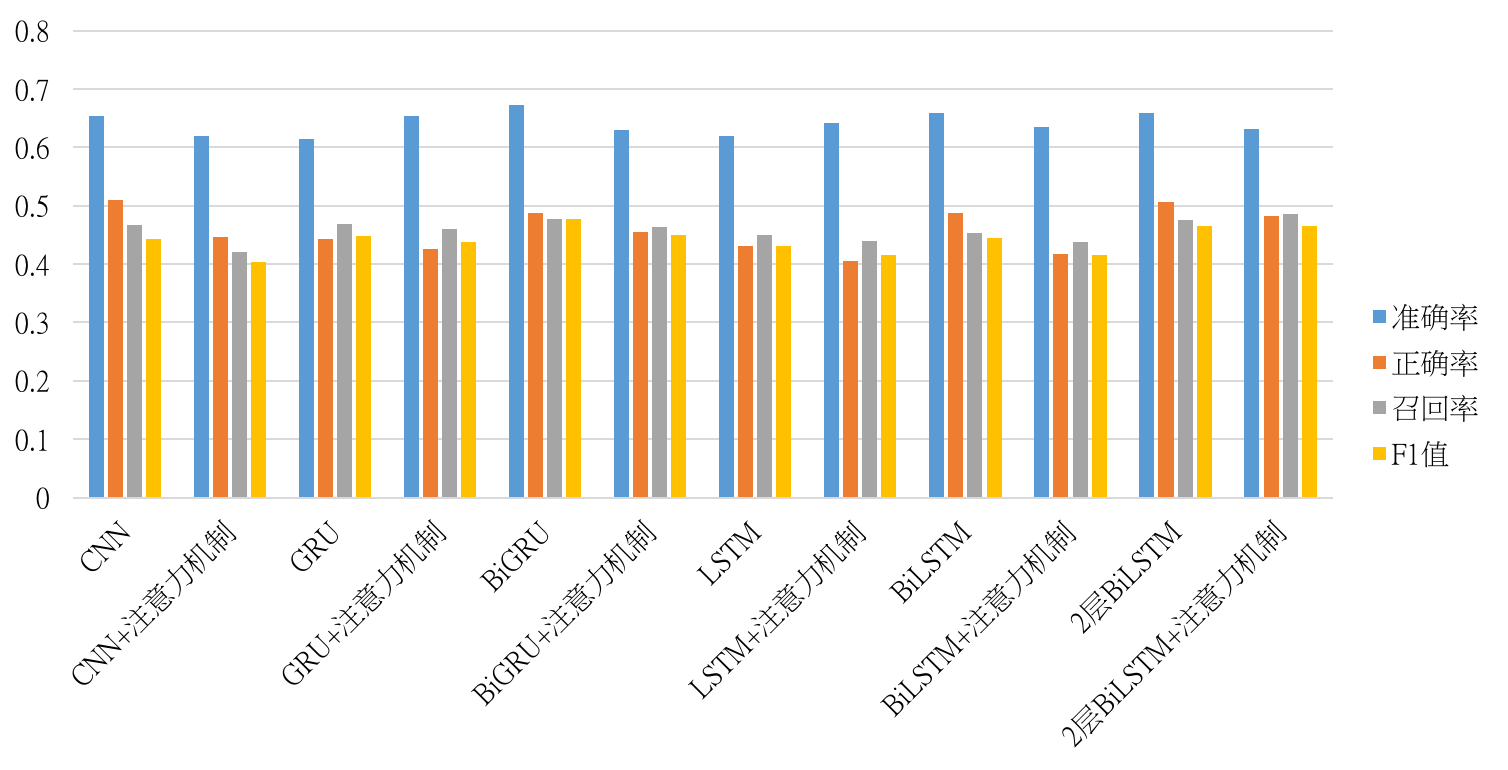
\includegraphics[width=\textwidth]{img/exp_irony_det_B_single_result_bar.png}
  \caption{面向反讽四分类的模型性能}
  \label{fig:exp_irony_det_B_single_result_bar}
\end{figure}

\subsubsection{面向“没有反讽”和“基于相反语义的反讽”二分类的实验结果分析}
\label{sssec:exp_irony_det_Bb01_base}

对于面向“没有反讽”和“基于相反语义的反讽”的二分类问题,表~\ref{tab:exp_irony_det_Bb01_result}和图~\ref{fig:exp_irony_det_Bb01_single_result_bar}显示不同卷积神经网络和迭归神经网络在测试集上能达到的性能。注意表中的正确率、召回率、F1值指两个类别对应指标数据的宏平均。

对于F1值,LSTM配合注意力机制达到最大数值的0.7752 ,其后依次为BiGRU和GRU,和前者差距约较小(0.005)。对于准确率,同样是LSTM配合注意力机制达到最好的效果(0.8275),其后依次为GRU和BiGRU,和前者差距大(0.015)。对于正确率,还是 LSTM配合注意力机制的数值最高(0.7717),其后依次为GRU和BiGRU,和前者差距大(0.015)。对于召回率,数值最高的是BiGRU(0.7993),其次是GRU和LSTM,和前者差距均较小(约0.005)。

总的来说,LSTM配合注意力机制在四项指标中的三项都达到了最好的性能,而各项指标的第二和第三基本上由GRU和BiGRU达到。由配合注意力机制的模型达到最好的性能,这一点和前面各个子分类问题的实验结果都不同,显示注意力机制可能对“基于相反语义的反讽”有相应的建模能力。另外GRU和BiGRU的性能非接近,从数学模型上看,BiGRU比单层GRU多一个把文本反向输入的GRU通道,提高了召回率的同时稍微降低了准确率和正确率,显示反向输入的GRU通道能额外捕足到“基于相反语义的反讽”相关的特征。但相对地BiLSTM在四项指标上都明显低于LSTM,我们认为其中的原因可能有两点,一是LSTM从数学模型上对“基于相反语义的反讽”的特征建模能力较差,二是BiLSTM的模型参数过多而导致对训练集的过拟合。

\begin{table}[htb]
  \centering
  \begin{minipage}[t]{\linewidth}
  \caption{面向“没有反讽”和“基于相反语义的反讽”的二分类各模型性能}
  \label{tab:exp_irony_det_Bb01_result}
    \begin{tabularx}{\linewidth}{X|llll}
    \toprule[1.5pt]
    & 准确率 & 正确率 & 召回率 & F1值 \\
    \hline
    CNN & 0.7991 (5) & 0.7438 (5) & 0.7791 (7) & 0.7562 (5) \\ % Bb01_cnn_ek_1554448736
    CNN+注意力机制 & 0.6829 (12) & 0.6494 (12) & 0.6909 (12) & 0.6470 (12) \\ % Bb01_cnn_ek_1554448788
    \hline
    GRU & 0.8100 (2) & 0.7566 (2) & 0.7944 (2) & 0.7699 (3) \\ % Bb01_gru_ek_1554448924
    GRU+注意力机制 & 0.7677 (9) & 0.7196 (9) & 0.7679 (10) & 0.7303 (9) \\ % Bb01_gru_ek_1554449053
    \hline
    BiGRU & 0.8085 (3) & 0.7565 (3) & \bf 0.7993 (1) & 0.7705 (2) \\ % Bb01_bgru_ek_1554449115
    BiGRU+注意力机制 & 0.7755 (8) & 0.7301 (8) & 0.7831 (5) & 0.7412 (8) \\ % Bb01_bgru_ek_1555407125
    \hline
    LSTM & 0.8053 (4) & 0.7525 (4) & 0.7932 (3) & 0.7661 (4) \\ % Bb01_lstm_ek_1554449707
    LSTM+注意力机制 & \bf 0.8257 (1) & \bf 0.7717 (1) & 0.7791 (7) & \bf 0.7752 (1) \\ % Bb01_lstm_ek_1554449864
    \hline
    BiLSTM & 0.7551 (10) & 0.7169 (10) & 0.7734 (9) & 0.7236 (10) \\ % Bb01_blstm_ek_1554449881
    BiLSTM+注意力机制 & 0.7174 (11) & 0.6909 (11) & 0.7460 (11) & 0.6889 (11) \\ % Bb01_blstm_ek_1554450198
    \hline
    2层BiLSTM & 0.7849 (7) & 0.7339 (7) & 0.7795 (6) & 0.7465 (7) \\ % Bb01_nblstm_ek_1554450231
    2层BiLSTM+注意力机制 & 0.7928 (6) & 0.7421 (6) & 0.7888 (4) & 0.7554 (6) \\ % Bb01_nblstm_ek_1554450448
    \bottomrule[1.5pt]
    \end{tabularx}
  \end{minipage}
\end{table}

\begin{figure}[H]
  \centering
  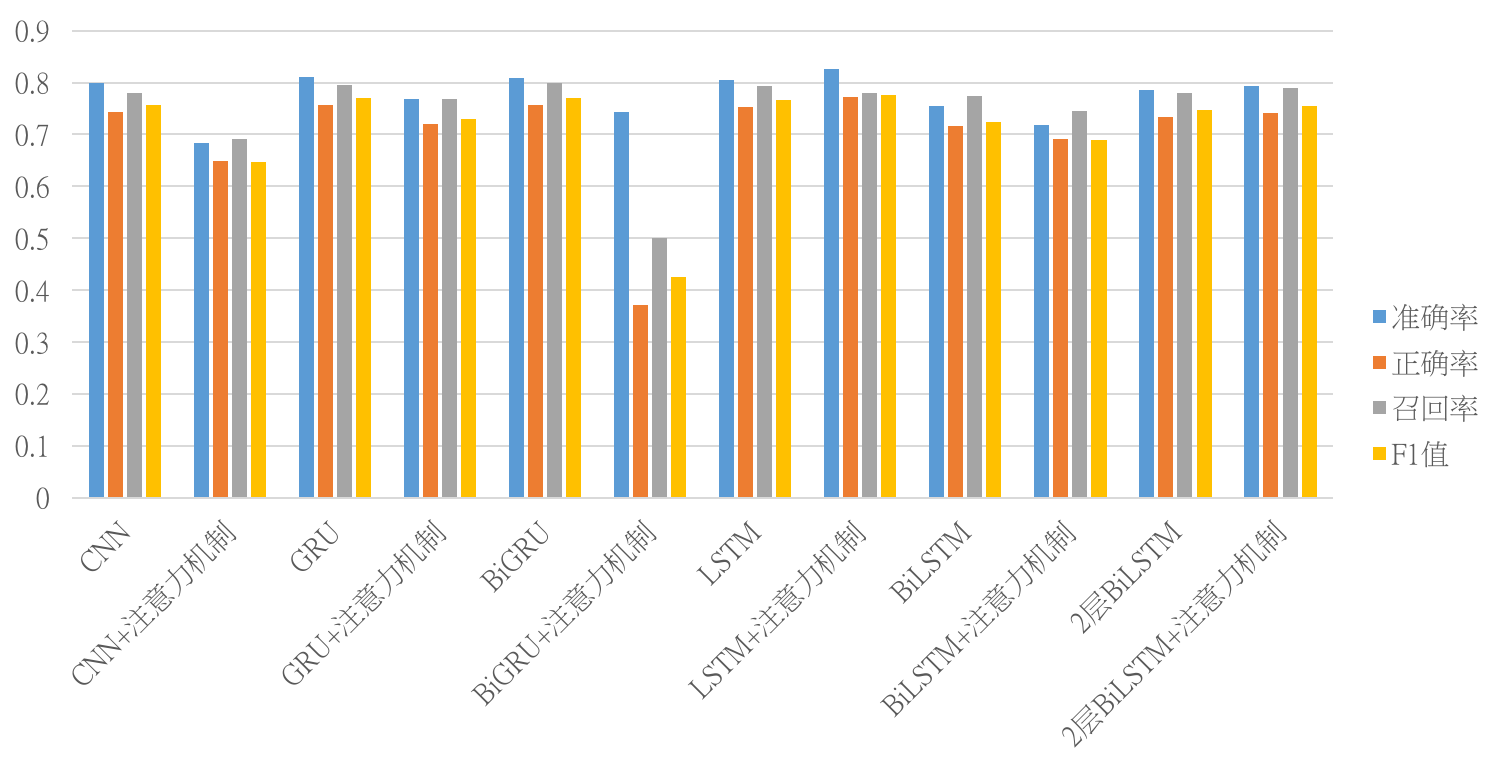
\includegraphics[width=\textwidth]{img/exp_irony_det_Bb01_single_result_bar.png}
  \caption{面向“没有反讽”和“基于相反语义的反讽”的二分类各模型性能}
  \label{fig:exp_irony_det_Bb01_single_result_bar}
\end{figure}

\subsubsection{面向“没有反讽”和“情景反讽”二分类的模型性能分析}
\label{sssec:exp_irony_det_Bb02_base}

对于面向“没有反讽”和“情景反讽”的二分类问题,表~\ref{tab:exp_irony_det_Bb02_result}和图~\ref{fig:exp_irony_det_Bb02_single_result_bar}显示不同卷积神经网络和迭归神经网络在测试集上能达到的性能。注意表中的正确率、召回率、F1值指两个类别对应指标数据的宏平均。

对于F1值和召回率,2层BiLSTM配合注意力机制在这两个指标上都达到了最好的效果(数值分别为0.6924 和 0.6806),其次是2层BiLSTM,第三是单层的BiLSTM配合注意力机制,但后两者在准确率和正确率这两项指标上都排在靠后的位置。而对于准确率和正确率,均由CNN达到最好的效果(数值分别为0.8656和 0.7634),其次是2层BiLSTM配合注意力机制,第三是单层的LSTM。

整体上,2层BiLSTM配合注意力机制在四项指标上的都达到了靠前的效果,显示2层BiLSTM配合注意力机制对“情景反讽”有明显较好的建模能力。另外CNN虽然在准确率和正确率上都达到最好的性能,但由于召回率数值太低导致了F1值明显低于第一的F1值(差距约0.045),显示CNN只对部分“情景反讽”的样本有较好的识别能力,导致了召回率偏低。

\begin{table}[htb]
  \centering
  \begin{minipage}[t]{\linewidth}
  \caption{面向“没有反讽”和“情景反讽”的二分类模型性能}
  \label{tab:exp_irony_det_Bb02_result}
    \begin{tabularx}{\linewidth}{X|llll}
    \toprule[1.5pt]
    & 准确率 & 正确率 & 召回率 & F1值 \\
    \hline
    CNN & \bf 0.8656 (1) & \bf 0.7634 (1) & 0.6167 (7) & 0.6473 (7) \\ % Bb02_cnn_ek_1554450719
    CNN+注意力机制 & 0.8477 (5) & 0.6865 (5) & 0.5917 (11) & 0.6117 (11) \\ % Bb02_cnn_ek_1554450772
    \hline
    GRU & 0.8495 (4) & 0.6942 (4) & 0.6024 (10) & 0.6242 (10) \\ % Bb02_gru_ek_1554450862
    GRU+注意力机制 & 0.8333 (11) & 0.6708 (8) & 0.6556 (4) & 0.6625 (4) \\ % Bb02_gru_ek_1554451013
    \hline
    BiGRU & 0.8423 (6) & 0.6645 (11) & 0.5789 (12) & 0.5951 (12) \\ % Bb02_bgru_ek_1554451047
    BiGRU+注意力机制 & 0.8423 (6) & 0.6825 (6) & 0.6416 (5) & 0.6572 (6) \\ % Bb02_bgru_ek_1554451155
    \hline
    LSTM & 0.8513 (2) & 0.7027 (3) & 0.6372 (6) & 0.6590 (5) \\ % Bb02_lstm_ek_1554451286
    LSTM+注意力机制 & 0.8387 (8) & 0.6676 (10) & 0.6153 (8) & 0.6325 (8) \\ % Bb02_lstm_ek_1554451194
    \hline
    BiLSTM & 0.8351 (10) & 0.6575 (12) & 0.6084 (9) & 0.6243 (9) \\ % Bb02_blstm_ek_1554451336
    BiLSTM+注意力机制 & 0.8369 (9) & 0.6797 (7) & 0.6674 (3) & 0.6731 (3) \\ % Bb02_blstm_ek_1554451401
    \hline
    2层BiLSTM & 0.8262 (12) & 0.6691 (9) & 0.6803 (2) & 0.6743 (2) \\ % Bb02_nblstm_ek_1554451496
    2层BiLSTM+注意力机制 & 0.8513 (2) & 0.7076 (2) & \bf 0.6806 (1) & \bf 0.6924 (1) \\ % Bb02_nblstm_ek_1554451575
    \bottomrule[1.5pt]
    \end{tabularx}
  \end{minipage}
\end{table}

\begin{figure}[H]
  \centering
  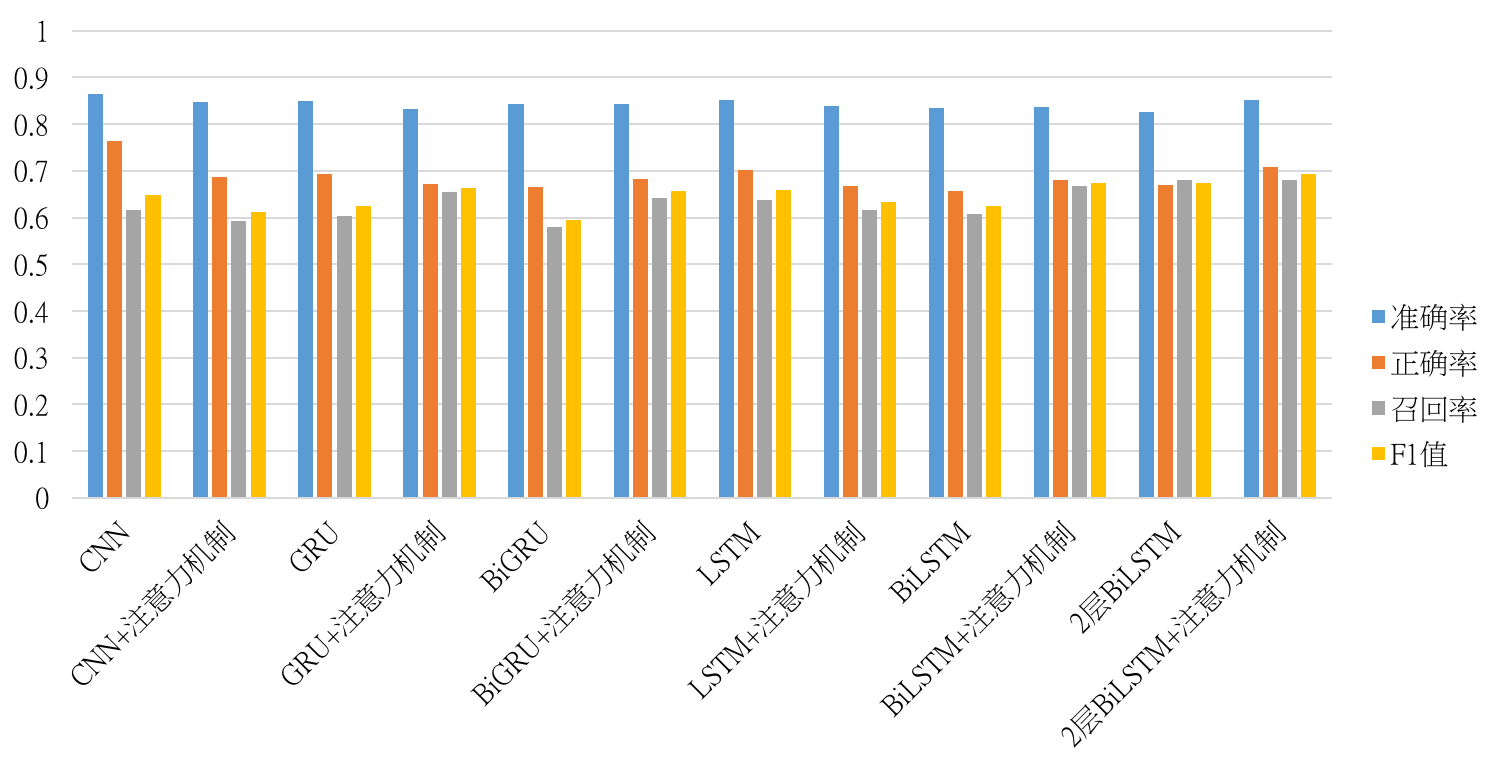
\includegraphics[width=\textwidth]{img/exp_irony_det_Bb02_single_result_bar.png}
  \caption{面向“没有反讽”和“情景反讽”的二分类模型性能}
  \label{fig:exp_irony_det_Bb02_single_result_bar}
\end{figure}

\subsubsection{面向“没有反讽”和“其他反讽”二分类的模型性能分析}
\label{sssec:exp_irony_det_Bb03_base}

对于面向“没有反讽”和“其他反讽”的二分类问题,表~\ref{tab:exp_irony_det_Bb03_result}和图~\ref{fig:exp_irony_det_Bb03_single_result_bar}显示不同卷积神经网络和迭归神经网络在测试集上能达到的性能。注意表中的正确率、召回率、F1值指两个类别对应指标数据的宏平均。

对于F1值,性能最好的是CNN(0.6016),其次是GRU,与前者差距明显(约0.016),第三为BiLSTM,明显低于CNN的数值(差距约为0.05)。对于准确率,同样是CNN达到最高的数值(0.8860),其次是GRU配合注意力机制以及LSTM配合注意力机制,在数值上比较接近(差距仅0.002)。对于正确率,依然是CNN的性能最优(0.7123),第二是GRU配合注意力机制,但和前者差距较明显(约0.02),第三的GRU则远差于前两者(差距达0.1以上)。 对于召回率,则是GRU的效果最好(0.5836),其次是CNN,与前者差距较小(约0.005),第三的BiLSTM则和前两者差距较大(达0.03以上)。

整体上,CNN在三项指标上的都达到了最好的效果,而在召回率也逼近最好的GRU,显示CNN对“其他反讽”有明显较好的建模能力。对于CNN在准确率和正确率上最佳,这和面向“没有反讽”和“情景反讽”的二分类实验结果相同,这可能有样本量分布有关,“情景反讽”和“其他反讽”的训练样本量(分别为316和205)都远少于“没有反讽”(1923),但CNN对“其他反讽”有较好的建模能力,因此在达到较好召回率的同时达到了最佳的F1值。

\begin{table}[htb]
  \centering
  \begin{minipage}[t]{\linewidth}
  \caption{面向“没有反讽”和“其他反讽”的二分类模型性能}
  \label{tab:exp_irony_det_Bb03_result}
    \begin{tabularx}{\linewidth}{X|llll}
    \toprule[1.5pt]
    & 准确率 & 正确率 & 召回率 & F1值 \\
    \hline
    CNN & \bf 0.8860 (1) & \bf 0.7123 (1) & 0.5781 (2) & \bf 0.6016 (1) \\ % Bb03_cnn_ek_1553500286
    CNN+注意力机制 & 0.7981 (11) & 0.4930 (8) & 0.4934 (11) & 0.4932 (7) \\ % Bb03_cnn_ek_1554453416
    \hline
    GRU & 0.8336 (10) & 0.5873 (3) & \bf 0.5836 (1) & 0.5853 (2) \\ % Bb03_gru_ek_1554452318
    GRU+注意力机制 & 0.8841 (2) & 0.6928 (2) & 0.5070 (7) & 0.4848 (8) \\ % Bb03_gru_ek_1554452300
    \hline
    BiGRU & 0.8411 (8) & 0.5481 (7) & 0.5317 (6) & 0.5353 (6) \\ % Bb03_bgru_ek_1554452373
    BiGRU+注意力机制 & 0.8822 (4) & 0.4419 (11) & 0.4989 (9) & 0.4687 (10) \\ % Bb03_bgru_ek_1554452659
    \hline
    LSTM & 0.8486 (6) & 0.5603 (5) & 0.5360 (4) & 0.5409 (4) \\ % Bb03_lstm_ek_1554452412
    LSTM+注意力机制 & 0.8841 (2) & 0.4421 (10) & 0.5000 (8) & 0.4692 (9) \\ % Bb03_lstm_ek_1554452800
    \hline
    BiLSTM & 0.8430 (7) & 0.5663 (4) & 0.5468 (3) & 0.5527 (3) \\ % Bb03_blstm_ek_1554452497
    BiLSTM+注意力机制 & 0.8822 (4) & 0.4419 (11) & 0.4989 (9) & 0.4687 (10) \\ % Bb03_blstm_ek_1554452804
    \hline
    2层BiLSTM & 0.8355 (9) & 0.5483 (6) & 0.5356 (5) & 0.5393 (5) \\ % Bb03_nblstm_ek_1554452506
    2层BiLSTM+注意力机制 & 0.7944 (12) & 0.4571 (9) & 0.4633 (12) & 0.4600 (12) \\ % Bb03_nblstm_ek_1554452977
    \bottomrule[1.5pt]
    \end{tabularx}
  \end{minipage}
\end{table}

\begin{figure}[H]
  \centering
  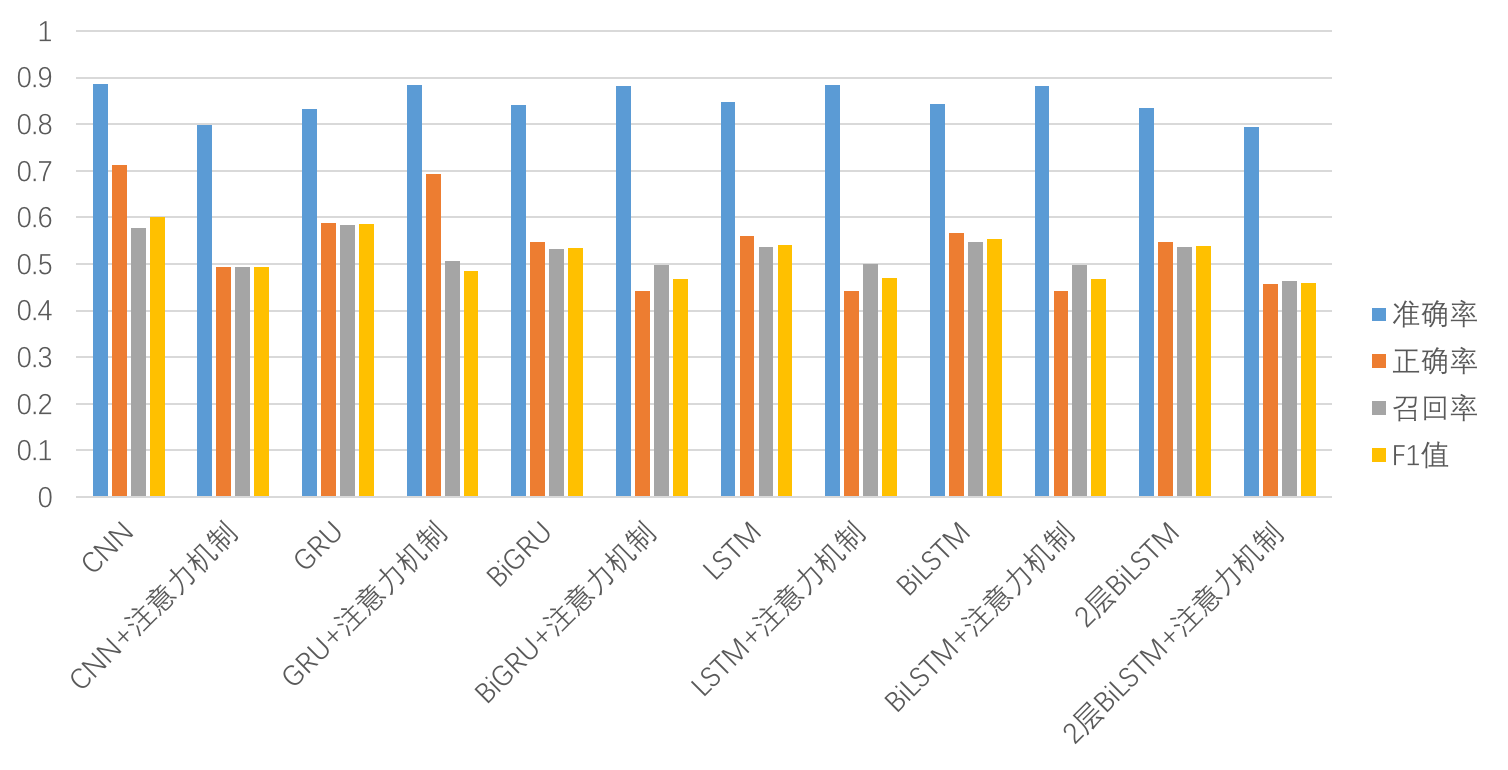
\includegraphics[width=\textwidth]{img/exp_irony_det_Bb03_single_result_bar.png}
  \caption{面向“没有反讽”和“其他反讽”的二分类模型性能}
  \label{fig:exp_irony_det_Bb03_single_result_bar}
\end{figure}

\subsubsection{面向“没有反讽”和“带有反讽”二分类的系统性能分析}

经过前面各章节的分析,我们已经对各个子分类问题中不同模型的性能有大致了解,接下来我们将基于子分类器实现反讽识别系统,并和比赛SemEval-2018任务三的参赛系统比较来评估我们系统的性能水平。

首先对于SemEval-2018任务三的子任务一,即面向“没有反讽”和“带有反讽”的二分类问题,基于章节~\ref{sssec:exp_irony_det_A_base}的实验结果,我们最终选择以F1值最高的2层BiLSTM作为子分类器的模型,按照章节~\ref{ssec:exp_irony_det_model_training}训练出由9个分类器组成的分类器组,按照章节~\ref{sec:exp_irony_det_framework},我由该分类器组的子分类器进行投票来得出一条微博的反讽类别。

表~\ref{tab:exp_irony_det_A_other_comp}显示我们的系统和SemEval-2018任务三子任务一其他参赛系统在测试集上的性能。注意表中的正确率、召回率、F1值均是针对类别“带有反讽”的指标。在SemEval-2018任务三子任务一的最终测试阶段,参赛系统共43个,表中仅显示排名前10(按照F1值排名)或在某项指标排名靠前的参赛系统,其中队伍名称为THU\_HCSI对应我们当时提交的系统,排名第8。

首先观察各项指标上我们系统的性能水平。对于F1值,我们系统的数值为0.7010,对应当时排名第二,略低于第一名的0.7050,显着高于当时第二名的0.6719(差距约0.03)。对于准确率,我们系统的数值为0.7256,对应当时排名第三,和第一名的差距约为0.009。对于正确率,我们系统的数值为0.6176,对应当时排名第五。对于召回率,我们系统的数值为0.8103,对应当时排名第四。总的来说我们的系统在上述四项指标上都达到了靠前的性能,对比我们提交的系统有了明显的提升。

另外对比单个子分类器(即单个2层BiLSTM模型对应的分类器)和整个系统的识别性能,系统在准确率、正确率和F1值都有明显的提升,只有召回率有轻微的下降,显示采用多数投票方法有效基于多个子分类器达到更好的识别性能。

\begin{table}[htb]
  \centering
  \begin{minipage}[t]{\linewidth}
  \caption{SemEval-2018任务三子任务一参赛系统性能} % 共43个参赛系统
  \label{tab:exp_irony_det_A_other_comp}
    \begin{tabularx}{\linewidth}{c|X|llll}
    \toprule[1.5pt]
    排名 & 队伍名称 & 准确率 & 正确率 & 召回率 & F1值 \\
    \hline 
    1 & THU\_NGN & \bf 0.7347 (1) & 0.6304 (4) & 0.8006 (4) & \bf 0.7054 \\
    2 & NTUA-SLP & 0.7321 (2) & 0.6535 (2) & 0.6913 (13) & 0.6719 \\
    3 & WLV & 0.6429 (15) & 0.5317 (20) & 0.8360 (2) & 0.6500 \\
    4 & (无) & 0.6607 (10) & 0.5506 (13) & 0.7878 (7) & 0.6481 \\
    5 & NIHRIO, NCL & 0.7015 (3) & 0.6091 (5) & 0.6913 (13) & 0.6476 \\
    6 & DLUTNLP-1 & 0.6276 (19) & 0.5199 (23) & 0.7974 (5) & 0.6294 \\
    7 & ELiRF-UPV & 0.6110 (23) & 0.5059 (27) & 0.8328 (3) & 0.6294 \\
    8 & \bf THU\_HCSI & 0.6594 (11) & 0.5550 (11) & 0.7138 (10) & 0.6245 \\
    9 & CJ & 0.6671 (8) & 0.5654 (9) & 0.6945 (12) & 0.6234 \\ 
    10 & \#NonDicevoSulSerio & 0.6786 (7) & 0.5831 (8) & 0.6656 (15) & 0.6216 \\
    \hline
    15 & (无) & 0.5651 (31) & 0.4731 (33) & \bf 0.8489 (1) & 0.6076 \\
    \hline
    43 & INGEOTEC-IIMAS & 0.6276 (19) & \bf 0.8800 (1) & 0.0707 (37) & 0.1310 \\
    \hline 
    & 单个分类器 & 0.6709 (8) & 0.5577 (10) & 0.8232 (4) & 0.6649 (3) \\ % A_nblstm_ek_1554346535
    & 我们的系统 & 0.7258 (3) & 0.6176 (5) & 0.8103 (4) & 0.7010 (2) \\
    \bottomrule[1.5pt]
    \end{tabularx}
  \end{minipage}
\end{table}

\subsubsection{面向反讽四分类的系统性能分析}

接下来我们分析面向反讽四分类的系统性能,对应SemEval-2018任务三的子任务二。按照章节~\ref{sec:exp_irony_det_framework},我们的反讽四分类系统涉及四个子分类问题。

对于和原问题相同的反讽四分类,根据章节~\ref{sssec:exp_irony_det_B_base}的实验结果,我们采用BiGRU的模型,作为第一组分类器。对于面向“没有反讽”和“基于相反语义的反讽”的二分类问题,按照章节~\ref{sssec:exp_irony_det_Bb01_base}的实验结果,我们采用LSTM配合注意力机制作为第二组分类器的模型。按照章节~\ref{sssec:exp_irony_det_Bb02_base}的实验结果,我们采用2层BiLSTM+注意力机制作为第三组分类器的模型。按照章节~\ref{sssec:exp_irony_det_Bb03_base}的实验结果,我们采用CNN作为第四组分类器的模型。按照章节~\ref{ssec:exp_irony_det_model_training},我们基于选定的模型分别为每个分类器组训练5个分类器。最后按照章节~\ref{sec:exp_irony_det_framework}中的设计的流程,经过各个组的投票结果逐步调整预测结果,最终得出一条微博的细分反讽类别。对于系统中对第二、三、四个分类器组需要配置的与置信度相关的参数$thr_2$、$thr_3$和$thr_4$ ,我们均设置为3,即完全相信第二、三、四个分类器组中过半数的投票结果。

表~\ref{tab:exp_irony_det_B_other_comp}显示我们的系统和SemEval-2018任务三子任务二其他参赛系统在测试集上的性能。注意表中的正确率、召回率、F1值均是针对各类别对应指标数据的宏平均。在SemEval-2018任务三子任务二的最终测试阶段,参赛系统共31个,表中仅显示排名前10(按照F1值排名)的参赛系统,而我们当时并未参与子任务二。
 
首先观察各项指标上我们系统的性能水平。
对于F1值,我们系统的数值为0.5499,对应当时排名第一,显着高于当时的第一名的0.5074。
对于准确率,我们系统的数值为0.6952,对应当时准确率排名第二,和最高数值的0.7321差距较大。
对于正确率,我们系统的数值为0.5600,对应当时正确率排名第二,和最高数值的0.5768有一定差距。
对于召回率,我们系统的数值为0.5402,对应当时召回率排名第二,和最高数值的0.5414差距较小。

总的来说我们的系统在上述四项指标上都达到了前二的性能,并在主要评价指标F1值上显着超过了当时的第一名。对比第一名的系统,我们系统的准确率和正确率都要低于前者,而召回率比它高,可以推断我们的系统成功召回了较多“带有反讽”的细分类别的样本,但同时把靠多真实标签为“没有反讽”的样本误判为“带有反讽”的细分类别。对于以较低的准确率换来较高的F1值,这与各类别的样本数量分布有关,由于“情景反讽”和“其他反讽”的样本量在测试集中占比较小而“没有反讽”的占比较大,以误判较多“没有反讽”的样本为代价召回更多“情景反讽”和“其他反讽”的样本能够明显提高最终的F1值。

\begin{table}[htb]
  \centering
  \begin{minipage}[t]{\linewidth}
  \caption{SemEval-2018任务三子任务二参赛系统性能} % 共31个参赛系统
  \label{tab:exp_irony_det_B_other_comp}
    \begin{tabularx}{\linewidth}{c|X|llll}
    \toprule[1.5pt]
    排名 & 队伍名称 & 准确率 & 正确率 & 召回率 & F1值 \\
    \hline 
    1 & (无) & \bf 0.7321 (1) & \bf 0.5768 (1) & 0.5044 (4) & \bf 0.5074 \\
    2 & NTUA-SLP & 0.6518 (4) & 0.4959 (4) & 0.5124 (2) & 0.4959 \\
    3 & \bf THU\_NGN & 0.6046 (9) & 0.4860 (6) & \bf 0.5414 (1) & 0.4947 \\
    4 & (无) & 0.6033 (10) & 0.4660 (7) & 0.5058 (3) & 0.4743 \\
    5 & NIHRIO, NCL & 0.6594 (3) & 0.5446 (2) & 0.4475 (5) & 0.4437 \\
    6 & Random Decision Syntax Trees & 0.6327 (6) & 0.4868 (5) & 0.4388 (8) & 0.4352 \\
    7 & ELiRF-UPV & 0.6327 (6) & 0.4123 (12) & 0.4404 (7) & 0.4211 \\
    8 & WLV & 0.6709 (2) & 0.4311 (10) & 0.4149 (9) & 0.4153 \\
    9 & \#NonDicevoSulSerio & 0.5446 (18) & 0.4087 (15) & 0.4410 (6) & 0.4131 \\
    10 & INGEOTEC-IIMAS & 0.6441 (5) & 0.5017 (3) & 0.3850 (15) & 0.4055 \\
    \hline
    & 我们的系统 & 0.6939 (2) & 0.5604 (2) & 0.5370 (2) & 0.5484 (1) \\
    \bottomrule[1.5pt]
    \end{tabularx}
  \end{minipage}
\end{table}

另外,由于我们的系统在经过每一步决策后的中间结果都可认作为一组预测结果,我们观察了每组中间结果在测试集上的性能。表~\ref{tab:exp_irony_det_B_ensemble_result}显示我们系统的中间结果在测试集上的各项指标,注意表中的正确率、召回率、F1值均是针对各类别对应指标数据的宏平均。

表中的第一行“中间结果I”对应直接由一组四分类器进行多数投票的识别结果,其F1值已超过原比赛中排名第一的数值。第二行“中间结果II”是基于第二个分类器组的投票对被判定为“没有反讽”和“基于相反语义的反讽”的样本重新进行二分类的识别结果,可见除了召回率以外的三项指标都有所提升。再对比中间结果I和中间结果II的混淆矩阵(分别对应表~\ref{tab:exp_irony_det_B_conf_mat_1}和表~\ref{tab:exp_irony_det_B_conf_mat_2})可以发现正确召回了9个“没有反讽”的样本,同时误判了3个原本识别正确的“基于相反语义的反讽”的样本,故整体准确率提升,但原本数值较低的“基于相反语义的反讽”的召回率下降拖低了整体的召回率。

表中的第三行“中间结果III”是基于第三个分类器组的投票对被判定为“没有反讽”和“情景反讽”的样本重新进行二分类的识别结果,可见准确率不变,正确率稍微下降,同时召回率有了明显提高,导致F1值也明显提高。再对比中间结果II和中间结果III的混淆矩阵(分别对应表~\ref{tab:exp_irony_det_B_conf_mat_2}和表~\ref{tab:exp_irony_det_B_conf_mat_3})可以发现误判了14个原本识别正确的“没有反讽”的样本,同时正确召回了14个“情景反讽”的样本,所以准确率不变,但由于“情景反讽”的样本总量较少而“没有反讽”的样本总量较多,“情景反讽”的召回率显着上升而拔高了宏平均的召回率,这也显示了对于宏平均的指标,关注样本量少的类别能在数值上带来明显提升。

表中的最底一行的“最终结果”是基于第四个分类器组的投票对被判定为“没有反讽”和“其他反讽”的样本重新进行二分类的识别结果,可见除了召回率不变,各项指标都有所提高。再对比中间结果III和最终结果的混淆矩阵(分别对应表~\ref{tab:exp_irony_det_B_conf_mat_3}和表~\ref{tab:exp_irony_det_B_conf_mat_4})可以发现这一步把5个被误判为“其他反讽”的样本都改成了“没有反讽”,虽然其中只有2个样本的真实标签为“没有反讽”,但由于被识别为“其他反讽”的样本少,明显提高了“其他反讽”的正确率。

总结以上结果,我們系統中对

\begin{table}[htb]
  \centering
  \begin{minipage}[t]{0.8\linewidth}
  \caption{四分类反讽识别系统最终识别结果和中间结果的性能}
  \label{tab:exp_irony_det_B_ensemble_result}
    \begin{tabularx}{\linewidth}{X|cccc}
    \toprule[1.5pt]
    & 准确率 & 正确率 & 召回率 & F1值 \\
    \hline
    中间结果I & 0.6837 & 0.5512 & 0.5016 & 0.5253 \\
    中间结果II & 0.6913 & \bf 0.5667 & 0.4920 & 0.5267 \\
    中间结果III & 0.6913 & 0.5512 & \bf 0.5370 & 0.5440 \\
    \hline
    最终结果 & \bf 0.6939 & 0.5604 & \bf 0.5370 & \bf 0.5484 \\
    \bottomrule[1.5pt]
    \end{tabularx}
  \end{minipage}
\end{table}

\begin{table}[]
  \centering
  \begin{minipage}[t]{0.8\linewidth}
  \caption{
    \label{tab:exp_irony_det_B_conf_mat_1}
    反讽四分类测试集上中间结果I对应的混淆矩阵
  }
  \begin{tabularx}{\linewidth}{c|c|cccc}
  \toprule[1.5pt]
  \multicolumn{2}{c|}{\multirow{2}{*}} & \multicolumn{4}{c}{预测标签}    \\
  \cline{3-6} 
  \multicolumn{2}{c|}{}
    & 没有反讽 & 相反语义 & 情景反讽 & 其他反讽  \\
  \hline
  \multirow{4}{*}{真实标签}
    & 没有反讽 & 380 & 73 & 13 & 7 \\
    & 相反语义 & 36 & 125 & 3 & 0 \\
    & 情景反讽 & 44 & 13 & 25 & 3 \\
    & 其他反讽 & 41 & 10 & 5 & 6 \\
  \bottomrule[1.5pt]
  \end{tabularx}
  \end{minipage}
\end{table}

\begin{table}[]
  \centering
  \begin{minipage}[t]{0.8\linewidth}
  \caption{
    \label{tab:exp_irony_det_B_conf_mat_2}
    反讽四分类测试集上中间结果II对应的混淆矩阵
  }
  \begin{tabularx}{\linewidth}{c|c|cccc}
  \toprule[1.5pt]
  \multicolumn{2}{c|}{\multirow{2}{*}} & \multicolumn{4}{c}{预测标签}    \\
  \cline{3-6} 
  \multicolumn{2}{c|}{}
    & 没有反讽 & 相反语义 & 情景反讽 & 其他反讽  \\
  \hline
  \multirow{4}{*}{真实标签}
    & 没有反讽 & 389 & 64 & 13 & 7 \\ 
    & 相反语义 & 39 & 122 & 3 & 0 \\
    & 情景反讽 & 47 & 10 & 25 & 3 \\
    & 其他反讽 & 39 & 12 & 5 & 6 \\
  \bottomrule[1.5pt]
  \end{tabularx}
  \end{minipage}
\end{table}

\begin{table}[]
  \centering
  \begin{minipage}[t]{0.8\linewidth}
  \caption{
    \label{tab:exp_irony_det_B_conf_mat_3}
    反讽四分类测试集上中间结果III对应的混淆矩阵
  }
  \begin{tabularx}{\linewidth}{c|c|cccc}
  \toprule[1.5pt]
  \multicolumn{2}{c|}{\multirow{2}{*}} & \multicolumn{4}{c}{预测标签}    \\
  \cline{3-6} 
  \multicolumn{2}{c|}{}
    & 没有反讽 & 相反语义 & 情景反讽 & 其他反讽  \\
  \hline
  \multirow{4}{*}{真实标签}
    & 没有反讽 & 375 & 64 & 27 & 7 \\
    & 相反语义 & 35 & 122 & 7 & 0 \\
    & 情景反讽 & 33 & 10 & 39 & 3 \\
    & 其他反讽 & 38 & 12 & 6 & 6 \\
  \bottomrule[1.5pt]
  \end{tabularx}
  \end{minipage}
\end{table}

\begin{table}[]
  \centering
  \begin{minipage}[t]{0.8\linewidth}
  \caption{
    \label{tab:exp_irony_det_B_conf_mat_4}
    反讽四分类测试集上最终识别结果对应的混淆矩阵
  }
  \begin{tabularx}{\linewidth}{c|c|cccc}
  \toprule[1.5pt]
  \multicolumn{2}{c|}{\multirow{2}{*}} & \multicolumn{4}{c}{预测标签}    \\
  \cline{3-6} 
  \multicolumn{2}{c|}{}
    & 没有反讽 & 相反语义 & 情景反讽 & 其他反讽  \\
  \hline
  \multirow{4}{*}{真实标签}
    & 没有反讽 & 377 & 64 & 27 & 5 \\
    & 相反语义 & 35 & 122 & 7 & 0 \\ 
    & 情景反讽 & 36 & 10 & 39 & 0 \\
    & 其他反讽 & 38 & 12 & 6 & 6 \\
  \bottomrule[1.5pt]
  \end{tabularx}
  \end{minipage}
\end{table}

% \subsection{错误分析}

\section{本章小结}

pass


\chapter{基于多通道模型引入上下文的情感识别}
\label{cha:exp_context_emo}

\section{本章引论}

在面向短文本的情感识别场景,有时候仅凭一段文本的内容可能无法完全理解发言者想表达的内容。考虑在一个甲乙两人对话的场景中,甲说“彼此彼此!”,我们可以认为甲表达了和乙相同的想法,但我们无法确认甲表达的情感。假如乙原本说“庆喜庆喜!”,那么可以认为甲也在表示祝贺,表达的是一种正面的情感。但假如乙原本说的是“你也不过如此!”,那么可以为甲在表示不满,表达的是一种负面的情感。因此在情感识别中,一些研究会考虑引入上下文信息作为辅助以提高识别性能。譬如Zahiri和Choi\cite{Zahiri2017Emotion}在研究电视剧剧本中每句台词的情感识别时,就引入了每句台词前的有限句台词作为上下文信息。Kunwoo等人\cite{hazarika2018conversational}在面向两人对话的情感识别研究中,同样引入了当前发言之前的有限段对话作为上下文信息。然而这些研究工作对上下文的建模方式都有所不同,如在Zahiri和Choi\cite{Zahiri2017Emotion}的研究中,一段剧本可能涉及多个角色,但在他们的模型中并没有考虑上下文中每句台词对应的角色,而在Kunwoo等人\cite{hazarika2018conversational}的研究中,由于对话过程只涉及两个人,在他们的模型中就区分了上下文中不同发言者说的话。对于不同场景下,如何在算法建模中引入上下文信息始终没有一种固定的方法,这也是因为不同类型的上下文包含的信息不同,对应具体的问题,我们依然需要进行针对性的模型设计。

国际比赛SemEval-2019的任务三\cite{SemEval2019Task3}则是旨在促进引入上下文的文本情感识别研究,比赛要求参赛者开发一个情感识别系统,对三轮对话中最后一轮发言表达的情感进行分类,给定的四个情感类别包括:开心、悲伤、愤怒、其他。为此我们提出了一个多通道模型,以引入作为上下文的前两轮对话。本章节中我们将基于SemEval-2019的任务三进行实验,采用比赛组织者提供的训练数据和测试数据,并透过和其他参赛系统进行比较来评估我们系统的识别性能。

本章的内容安排如下。在章节~\ref{sec:exp_context_emo_format}中,我们会首先给出当前问题的形式化表示。在章节~\ref{sec:exp_context_emo_data}中我们再对具体实验数据进行观察,分析给定数据集中各个情感类别的分布情况以及其文本特征等。在章节~\ref{sec:exp_context_emo_framework}将给出我们针对当前问题提出的多分类器分层识别算法,以及组成该最终识别系统的多通道分类模型。最后在章节~\ref{sec:exp_context_emo_exp},我们会给出实验的细节,以及对实验结果进行分析。

\section{形式化表示}
\label{sec:exp_context_emo_format}

在本章中,我们将研究面向三轮对话的情感识别,以下我们对应章节~\ref{sec:global_problem_analysis}给出此问题的形式化表示。给定一个情感类别集合$C$,对于一个三轮对话的集合$S$,其中任意一个元素$s$可以表示为一个三元组$<t^1, t^2, t^3>$,三元组中的元素依次对应每轮发言的文本内容。而在上下文为$b=<t^1, t^2>$的情况,最后一轮发言$t^3$所表达的情感属于唯一一种情感类别$c \in C$。又给定一个词集合$W$,对任意一轮发言的文本$t^j, j=1,2,3$,经过文本预处理后可以表示为一个长度为$L^j$的词序列 $w^j = <w^j_1, w^j_2, ..., w^j_{L^j}>, w^j_i \in W, i \in [1, L^j]$。那么我们的目标是找出一个映射关系$f$,使得$c=f(w^3, <w^1, w^2>)$。

\section{实验数据}
\label{sec:exp_context_emo_data}

我们的实验采用SemEval-2019的任务三提供的数据集,其中每个样本对应一个三轮对话以及第三轮发言的情感标签,第一轮为用户甲的发言,第二轮为用户乙对第一轮的回复,第三轮为用户甲对第二轮中用户乙的回复。情感标签对应四个情感类别中的其中一种:开心、悲伤、愤怒、其他。表~\ref{tab:semeval_2019_task3_data}显示数据集各类别样本数量分布,表~\ref{tab:semeval_2019_task3_sample}为语料中各个类别对应的样本例子。

\begin{table}[htb]
  \centering
  \begin{minipage}[t]{0.8\linewidth}
  \caption{情感识别各类别样本数量分布}
  \label{tab:semeval_2019_task3_data}
    \begin{tabularx}{\linewidth}{X|XXXX}
    \toprule[1.5pt]
    数据集 & 其他 & 开心 & 悲伤 & 愤怒 \\  
    \hline
    训练集 & 14948 & 4243 & 5463 & 5506 \\
    验证集 & 2338 & 142 & 125 & 150 \\
    测试集 & 4677 & 284 & 250 & 298 \\
    \bottomrule[1.5pt]
    \end{tabularx}
  \end{minipage}
\end{table}

\begin{table}[]
  \centering
  \begin{minipage}[t]{0.7\linewidth}
  \caption{各情感类别对应的三轮对话例子}
  \label{tab:semeval_2019_task3_sample}
  \begin{tabularx}{\linewidth}{c|l}
  \toprule[1.5pt]
   类别 & 对话    \\
  \hline
  \multirow{3}{*}{开心} 
    &   (第一轮)用户甲: live in uttra khand \\
    &   (第二轮)用户乙: ohh nice! love that place! \\
    &   (第三轮)用户甲: 
\includegraphics[height=1.5\fontcharht\font`\B]{img/emoji/lol.png}
\includegraphics[height=1.5\fontcharht\font`\B]{img/emoji/lol.png} \\
  \hline
  \multirow{3}{*}{悲伤} 
    &   (第一轮)用户甲: Not coz of you  \\
    &   (第二轮)用户乙: why? Tell me  \\
    &   (第三轮)用户甲: :( My girlfriend left me \\
  \hline
  \multirow{3}{*}{愤怒} 
    &   (第一轮)用户甲: He is over me \\
    &   (第二轮)用户乙: so YOU say \\
    &   (第三轮)用户甲: I just hate him \\
  \hline
  \multirow{3}{*}{其他} 
    &   (第一轮)用户甲: degreee \\
    &   (第二轮)用户乙: what degree \& where? \\
    &   (第三轮)用户甲: sryyy i really got to goo \\
  \bottomrule[1.5pt]
  \end{tabularx}
  \end{minipage}
\end{table}


在训练集上“其他”、“开心”、“悲伤”、“愤怒”四个类别的样本数量分布约为3:1:1:1 ,而在验证集和测试集上四个类别的样本数量分布约为22:1:1:1 。可见在验证集和测试集上“其他”一类的样本数量要远高于其他三个类别,和训练集相比其样本占比也相对较高,而另外三个类别的样本数量在各个数据集上则大致相同。

在比赛的最终测试阶段,训练集和验证集均已公布情感标注并且被允许用于模型训练,因此我们结合了原本的训练集和验证集作为我们的训练数据。

\subsection{文本长度}

我们对数据集的文本进行分词后统计了各类别样本的单词数量分布,以下简称为文本长度。表\ref{fig:context_emo_train_class_len}显示在训练集上各情感类别的样本在每轮发言的文本长度分布,可以看出在每轮发言中,不同类别样本的文本长度分布大致相同。虽然第一轮和第三轮的样本中最长的文本分别达到146个词和74个词,但各轮样本的文本长度大部分在22个词以内,约为前一章实验数据中样本文本长度的一半。

\begin{figure}[h]
  \centering%

  \begin{minipage}{\linewidth}

  \subcaptionbox{第一轮\label{fig:context_emo_train_class_len_0}} %[3cm] 
    {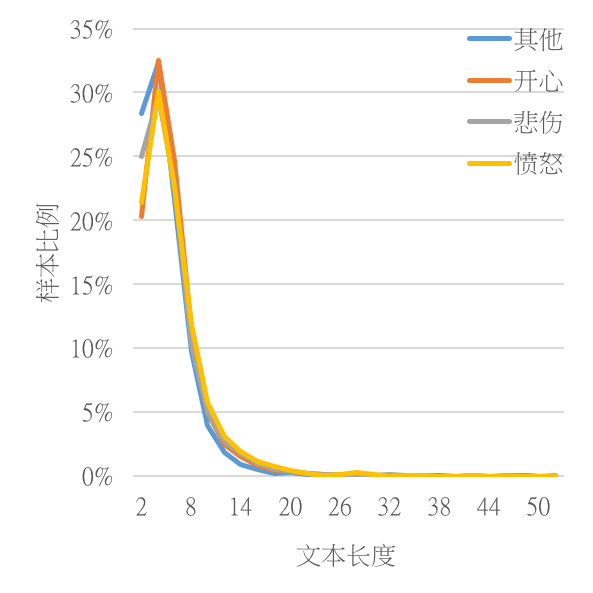
\includegraphics[height=8cm]{img/semeval2019_task3_train_0_class_len.png}}%
  %\hspace{em}%
  \subcaptionbox{第二轮\label{fig:context_emo_train_class_len_1}}
      {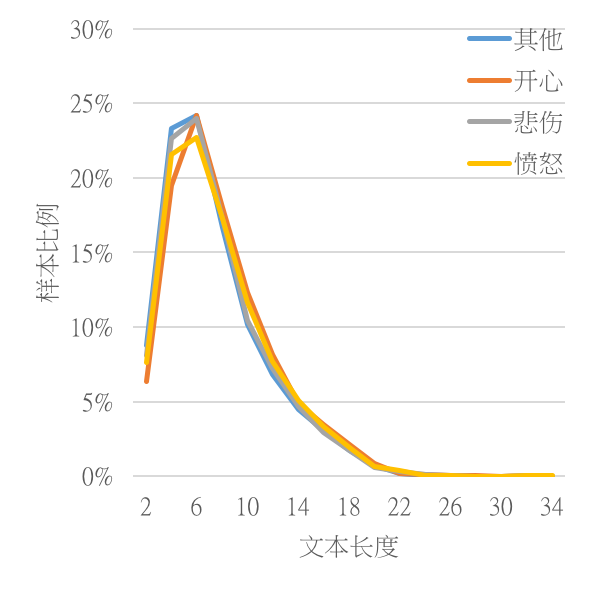
\includegraphics[height=8cm]{img/semeval2019_task3_train_1_class_len.png}}

  \end{minipage}
  \vspace{0.5cm} 

  \subcaptionbox{第三轮\label{fig:context_emo_train_class_len_2}}
      {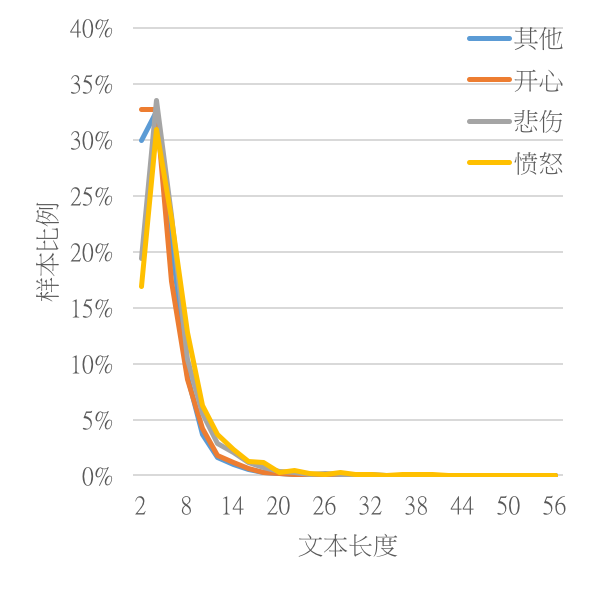
\includegraphics[height=8cm]{img/semeval2019_task3_train_2_class_len.png}}

  \caption{训练集上各情感类别的样本在每轮发言的文本长度分布}

  \label{fig:context_emo_train_class_len}
\end{figure}

\subsection{文本特征}
\label{ssec:exp_context_emo_data_text}

对于比赛中提供的数据集,比赛组织者并没有给出数据的具体来源,但经过人工观察后我们可以发现一些社交网络上常见的文本特征,其中出现频率较高的特征如下:

\begin{itemize}

\item 大量的缩略词使用,如“u”代替“you”,“y”代替“why”,“im”代替“I am”。

\item 出现在句子最前或最后的表情符,其中包括Unicode定义表情符(如
\includegraphics[height=1.5\fontcharht\font`\B]{img/emoji/lol.png})和由标点符号组成的表情符(如“:-D”)两类。

\item 一些在社交媒体平台上常见的、有别于正规英语的用法,如拼写错误、全大写字母的单词等,可以参考章节\ref{ssec:text_preprocess}描述的例子。

\end{itemize}

\subsection{各轮发言间的情感信息}
\label{ssec:exp_context_emo_multi_turn_analyse}

为了结合三轮对话中前两轮的发言来预测最后一轮发言的情感,我们需要观察各轮发言是否关最后一轮发言的情感有关,若有关的话各轮发言是否起着相同的作用。以下我们将采用数据集中的具体例子说明我们对语料的观察和理解。

首先,对于三轮发言中两个用户的情感,我们发现用户甲和用户乙表达的情感可能截然不同,参考以下例子:

\makebox[4 cm]{(第一轮)用户甲:} yes yay fun\par
\makebox[4 cm]{(第二轮)用户乙:} are not you joining us? :( \par
\makebox[4 cm]{(第三轮)用户甲:} yes\par

用户甲在最后一轮发言的情感标签为“开心”,而第一轮发言在字面意思上同样偏向正面。而对于用户乙在第二轮的发言,根据上下文意思和最后文本末尾的“:(”,我们可以推断用户乙的情感为“伤心”。可见三轮对话中两个用户表达的情感可能不同甚至矛盾,因此用户甲的发言和用户乙的发言对识别第三轮发言的情感应起着不同的作用,第二轮中用户乙的发言甚至没有提示的作用。

另外对于用户甲,我们发现他在第一轮和第三轮中表达的情感也有可能不同,参考以下例子:

\makebox[4 cm]{(第一轮)用户甲:} not fine\par
\makebox[4 cm]{(第二轮)用户乙:} why? :'o \par
\makebox[4 cm]{(第三轮)用户甲:} tomorrow lab exam\par

用户甲在最后一轮发言的情感标签为“悲伤”,而在字面意思上,最后一轮发言的情感偏中性,只是在陈述“明天有考试”的事情,“悲伤”的情感提示主要来自用户甲在第一轮中表示自己的情况“不太好”,第三轮发言在解释“不太好”的原因。基于此例子可以认为,同为用户甲发言的第一轮在某此情况下对识别第三轮发言的情感起着决定性作用。再观察下面的例子:

\makebox[4 cm]{(第一轮)用户甲:} ohh sorry\par
\makebox[4 cm]{(第二轮)用户乙:} do not worry, you are not the first \par
\makebox[4 cm]{(第三轮)用户甲:} glad to hear\par

用户甲在最后一轮发言的情感标签为“开心”,对于用户甲在第一轮发言表达的情感,结合用户乙在第二轮的发言,可以认为用户甲在第一轮发言中表示对用户乙的同情,这与“开心”为不同的情感,而在用户乙发言后,用户甲的情感因为用户乙说的话而转换成“开心”。可见用户甲在第一轮和第三轮中表达的情感有可能不同,这种情感的转变可能由用户乙的发言造成,但无论具体原因是什么,用户甲在第一轮和第三轮中的发言对识别第三轮发言的情感应起着不同的作用。

再者,我们发现用户甲在第三轮发言中可能出现多于一种情感,参考以下例子:

\makebox[4 cm]{(第一轮)用户甲:} 
\includegraphics[height=1.5\fontcharht\font`\B]{img/emoji/laugh.png} yes yes \par
\makebox[4 cm]{(第二轮)用户乙:} :3 you seem like a happy person \par
\makebox[4 cm]{(第三轮)用户甲:} yes 
\includegraphics[height=1.5\fontcharht\font`\B]{img/emoji/lol.png} happy outside, 
\includegraphics[height=1.5\fontcharht\font`\B]{img/emoji/frown.png} sad inside \par

用户甲在最后一轮发言的情感标签为“悲伤”,而在文本上,第三轮发言的前半表现为正面情感,后半表现为负表情感,前后的情感不同。对于当第三轮发言中出现两种情感时情感标签以何者为准,比赛组织者并没有给出细节的说明,但对语料的观察可以发现普遍以后面出现的情感为主。

最后总结我们对语料的观察,我们发现三轮发言对识别第三轮发言的情感应起着不同的作用。当第三轮发言有明显的情感表达,我们可以无视前两轮的发言得出识别结果。当第三轮发言表达的情感较隐晦或偏中性,需要参考同为用户甲发言的第一轮的信息。第二轮发言对第三轮发言的情感识别未有明显的提示作用。

\section{框架设计}
\label{sec:exp_context_emo_framework}

同样地,我们提出了一个多分类器分层识别算法。对于原本的情感四分类问题,我们把它拆解成了以下三个子分类问题的叠加:

\begin{enumerate}

\item 原本的情感四分类问题。
\item “开心”、“悲伤”和“愤怒”三分类。
\item “其他”和“不是其他”二分类。

\end{enumerate}

对于每个子分类问题,我们分别准备其对应的分类器组,依次命名为第一、第二、第三组分类器,分别由$N_1$、$N_2$、$N_3$个分类器组成。那么对于三轮对话中最后一轮发言的情感识别,我们系统的决策过程如下:

\begin{itemize}

\item 首先由对应原四分类问题的第一组分类器进行多数投票,得出预测标签$Label^{1}_{MV}$,直接以它作为第一步的预测标签$Label_{I}$ 。以下把算法到这一步为止的判断结果称为中间结果I。

\item 第二步,由面向“开心”、“悲伤”和“愤怒”三分类的第二组分类器进行多数投票,得出预测标签$Label^{2}_{MV}$,若超过$thr_{2}$分类器投票投给$Label^{2}_{MV}$且第一步的预测标签$Label_{I}$为“其他”以外的三种情感类别之一,则把预测结果修改为$Label^{2}_{MV}$,否则保持不变,以此得出第二步的预测标签$Label_{II}$。以下把算法到这一步为止的判断结果称为中间结果II。

\item 最后一步,由面向“其他”和“不是其他”二分类的第三组分类器给出投票结果,若超过$thr_{3}$个分类器投票给“其他”且第二轮的预测标签$Label_{II}$不是“其他”,则把预测标签修改为“其他”,否则保持不变,以此得出第三步的预测标签$Label_{III}$,同时作为整个算法对第三轮发言最终的情感识别结果。

\end{itemize}

整个决策过程可以分成两大部分。第一部分的目的是初步完成对第三轮发言的四分类情感识别,对应上述三步决策中的第一步。第二部分的目的是基于第一部分的初步识别结果逐步进行修正,每一步只关注一个子分类问题,对应上述三步决策中的后两步。其中第二步进行“开心”、“悲伤”和“愤怒”的三分类,目的在于调整三个类别之间的识别结果。而在最后一步进行“其他”和“不是其他”二分类,但特别地不是取多数投票,而是只要超过$thr_{3}$个分类器投票给“其他”即把识别标签改成“其他”,目的在于提高系统对“其他”一类的召回率。

\begin{figure}[H]
  \centering
  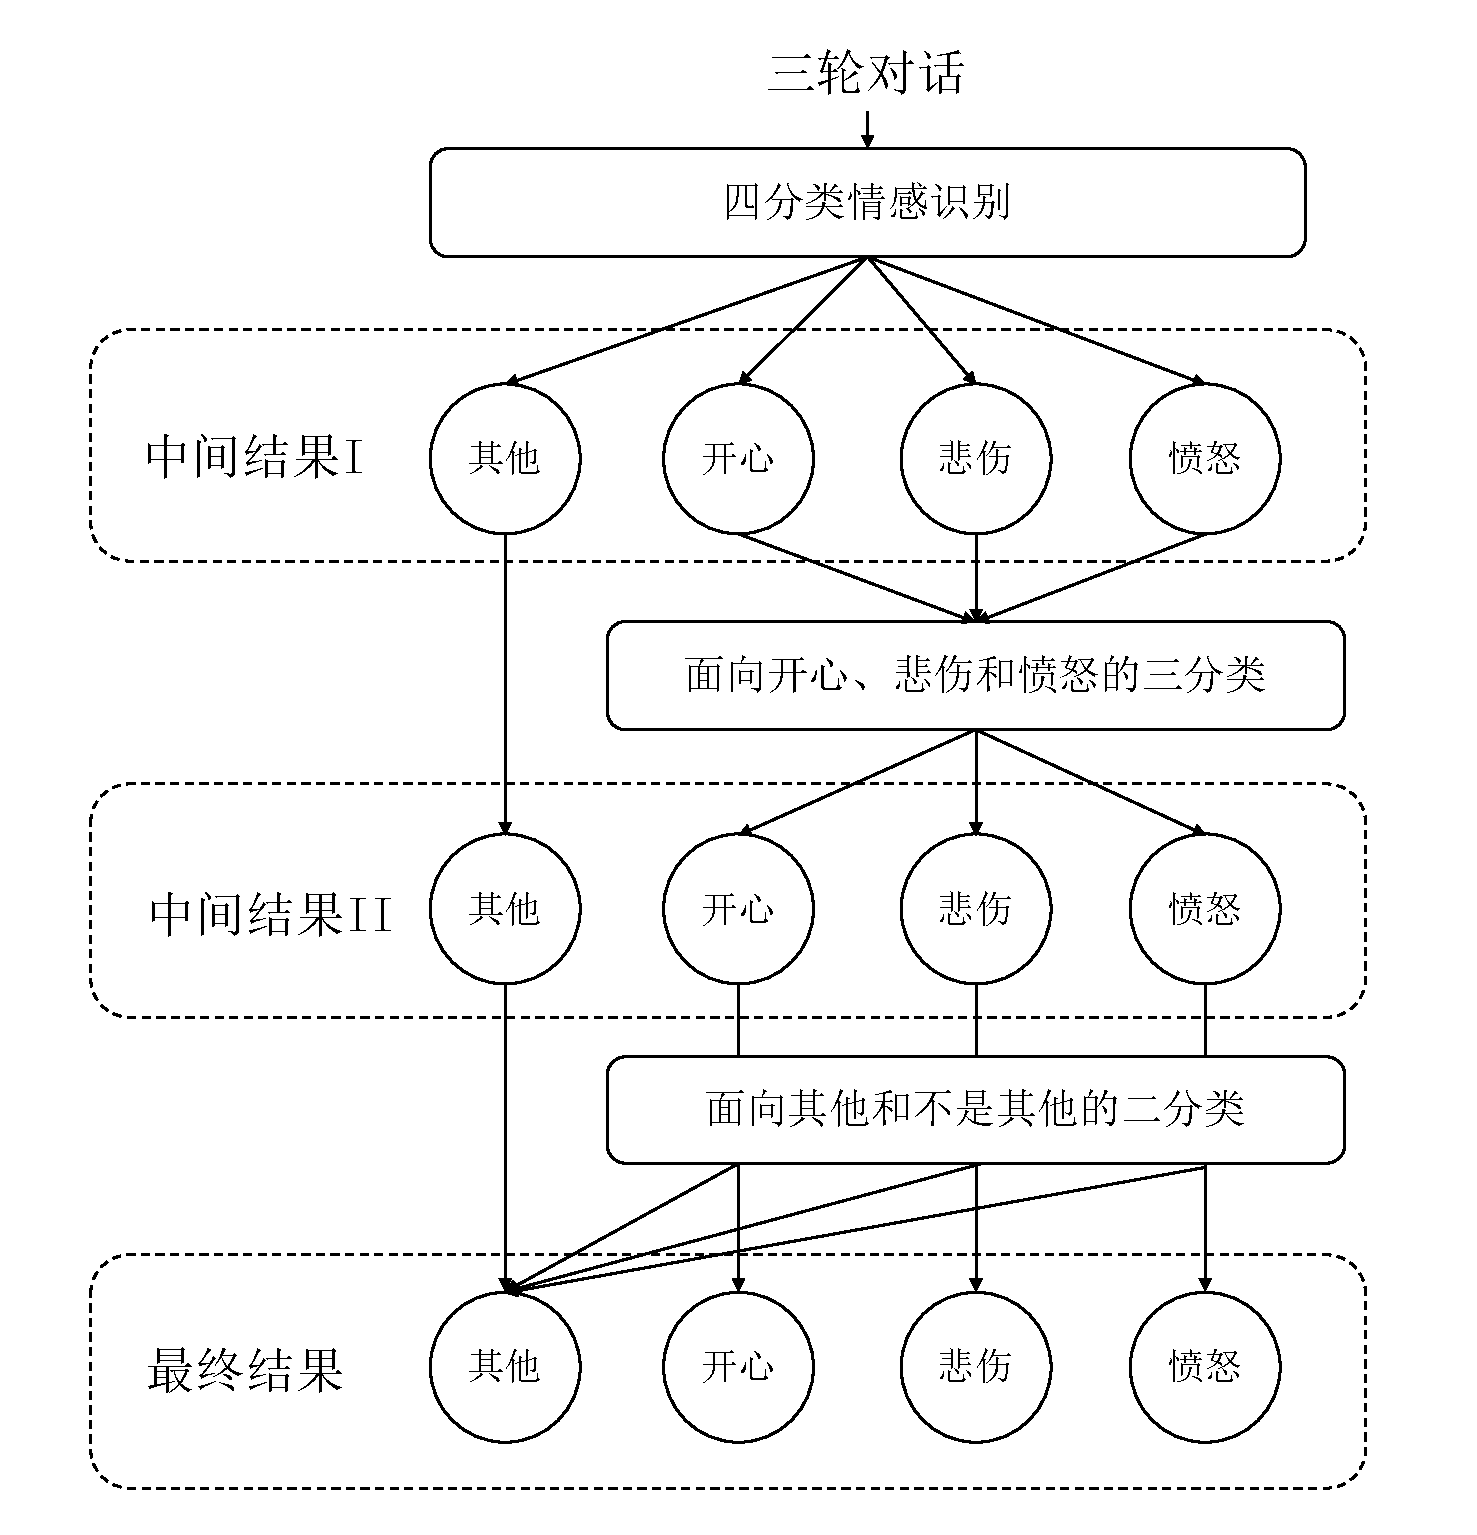
\includegraphics[width=0.9\textwidth]{img/context_emo_system.pdf}
  \caption{三轮对话的情感识别系统框架}
  \label{fig:context_emo_system}
\end{figure}

其中对于每个子分类问题,我们都采用了我们提出的多通道分类模型框架,如图\ref{fig:context_emo_cls_framework}所示,每个子分类器的输入为三轮对话对应的词序列$\{w^1, w^2, w^3\}$。根据在章节\ref{ssec:exp_context_emo_multi_turn_analyse}中的分析,我们认为三轮发言对识别第三轮发言的情感识别起着不同的作用,因此三轮发言对应的词序列分别进入不同的通道。每个通道的结构相同,第一步都是把词序列转换成对应的词嵌入向量序列,作为特征编码器的输入。此处特征编码器的设计与章节\ref{sec:exp_irony_det_framework}中的相同,目的是把单轮发言对应的词向量序列转换成固定长度的特征向量,以此得出该轮发言的特征向量。为了简化,三个通道的特征编码器采用相同的模型,但考虑到每轮发言对第三轮情感有关的特征可能不同,三个通道的模型各自采用不同的权重。分别得出三轮发言的特征向量后我们需要结合这些特征来识别第三轮的情感类别,此处我们直接把三个向量拼接成一个向量,作为概率预测器的输入。此处概率预测器的设计与章节\ref{sec:exp_irony_det_framework}中的相似,但实现上采用了两层的全联接层,第一层的激活函数为线性整流函数(Rectified Linear Unit, ReLU),而第二层的激活函数依然为$Softmax$,以得出各个情感类别的概率分布。

考虑到对于不同情感类别的语言特征不同,各个模型的建模能力也会有所不同。所以对于每个子分类问题,我们会分别比较各个模型的性能,以求在子分类问题上达到尽可能好的识别性能。

\begin{figure}[H]
  \centering
  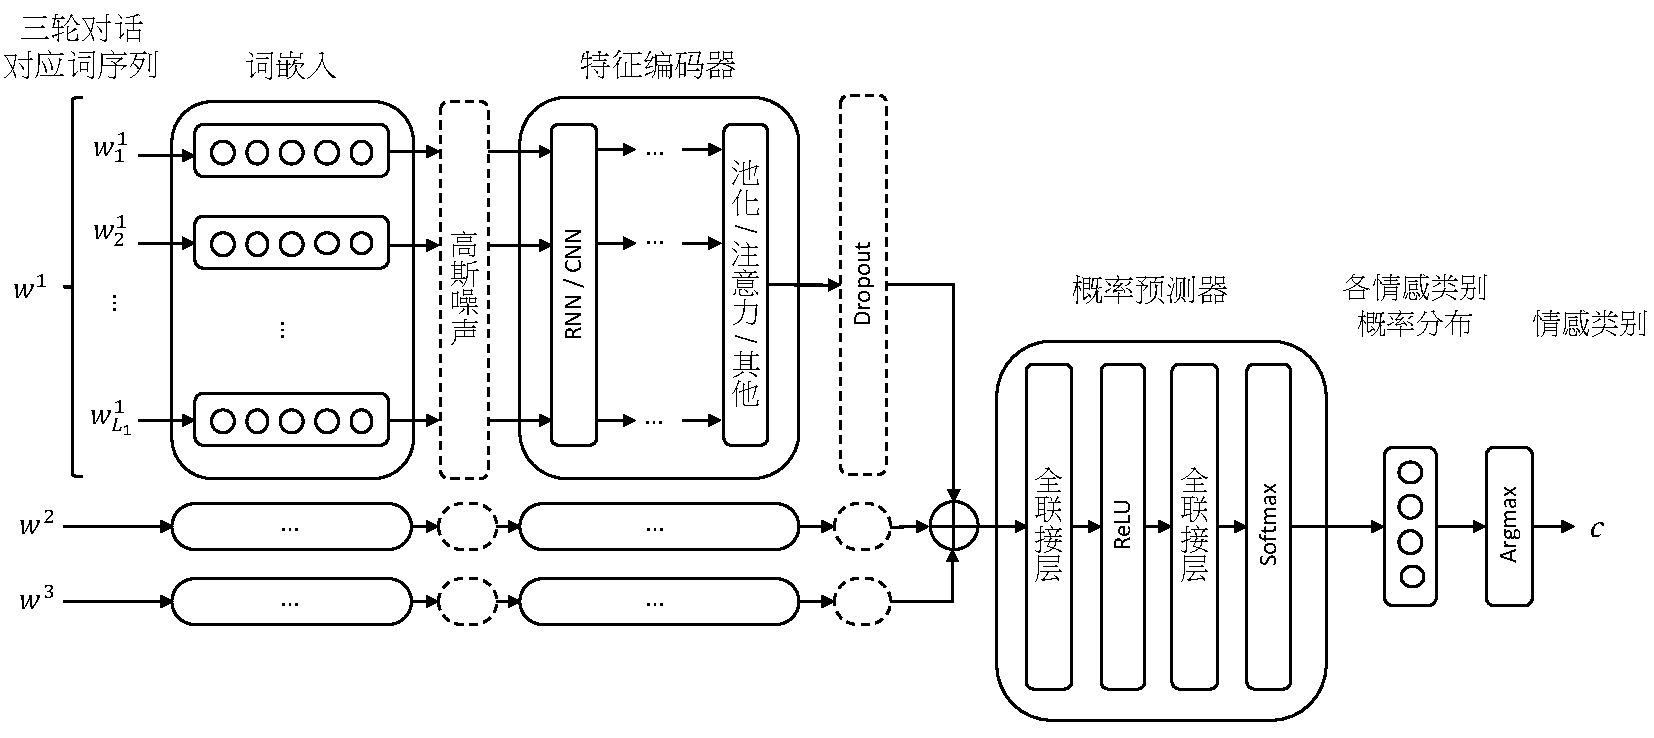
\includegraphics[width=\textwidth]{img/context_emo_cls_framework.pdf}
  \caption{面向三轮对话情感识别的多通道分类模型框架}
  \label{fig:context_emo_cls_framework}
\end{figure}

\section{实验与分析}
\label{sec:exp_context_emo_exp}

\subsection{数据预处理}

基于我们在章节\ref{ssec:exp_context_emo_data_text}中对样本文本的观察,我们依次采取了以下数据预处理手法

\begin{itemize}

\item 对于全字母大写的文本段,在该段文本的前后添加“<allcap>”和“</allcap>”示意。如“YAYYYY”替换成序列“<allcap>”、“yayyyy”、“</allcap>”。

\item 对于重复次数大于等次三次的标点符号,以“<repeated>”示意,如“!!!”替换成序列“!”、“<repeated>”,表示“!”被多次重复,即时假设重复的具体次数和原微博的反讽类别无关。

\item 对于字母被故意重复的单词,以“<elongated>”示意,如“Noooooooo”替换成序列“No”、“<elongated>”,表示“No”中某一个或多个字母被多次重复,即假设被重复的字符和具体重复的次数和原微博的反讽类别无关。

\item 将数字串替换成“<num>”,将电话号码替换成“<phone>”,将日期和时间分别替换成“<date>”和“<time>”,将数字百分比替换成“<percentage>”,超链接替换成“<url>”,即假设其中的具体数值和原微博的反讽类别无关。

\item 对于由多个标点符号组成的表情符,我们将其替换成对应的情感标签,如将“:)”替换成“<happy>”,“:((”替换成“<sad>”。

\item 在完成以上处理后,对英文的大小写统一转换成小写。

\end{itemize}

具体实现和章节~\ref{ssec:exp_irony_det_text_preprocess}中的相同。

\subsection{评价指标}
\label{ssec:exp_context_emo_eval_metric}

按照国际比赛SemEval-2019任务三的设置,系统性能以针对“开心”、“悲伤”和“愤怒”三个情感类别的F1值(以下记为 $F_\mu$)作为识别系统性能的主要评价指标。其定义如下:

\begin{align}
  F_\mu &= \frac{2 \times P_\mu \times R_\mu}{P_\mu + R_\mu}
\end{align}

其中 $P_\mu$ 和 $R_\mu$ 分别是针对“开心”、“悲伤”和“愤怒”三个情感类别的正确率和召回率,其定义如下:

\begin{align}
  P_\mu &= \frac{\sum\limits_{c \in C} TP_c}{\sum\limits_{c \in C}(TP_c + FP_c)} \\
  R_\mu &= \frac{\sum\limits_{c \in C} TP_c}{\sum\limits_{c \in C}(TP_c + FN_c)}
\end{align}

其中 $C$对应情感类别集合\{开心,悲伤,愤怒\},$TP_c$表示被系统预测为类别$c$,且真实标签为类别$c$的样本数量;$FP_c$表示被系统预测为类别$c$,但真实标签不是类别$c$的样本数量;$FN_c$被系统预测为不是类别$c$,但真实标签为类别$c$的样本数量。 

%另外,原比赛虽然以 $F_\mu$ 为排名的主要指标,但比赛组织者同样关注各个情感类别的F1值,因此在以下实验结果分析中我们也会这些指示进行观察,从而以不同角度了解系统识别性能。各个情感类别的F1值定义如下:

%\begin{align}
%  F_c &= \frac{2 \times P_c \times R_c}{P_c + R_c}
%\end{align}

%其中 $P_c$ 为类别$c$的正确率,$R_c$ 为类别$c$的召回率,其定义如下:

%\begin{align}
%  P_c &= \frac{TP_c}{TP_c + FP_c} \\
%  R_c &= \frac{TP_c}{TP_c + FN_c}
%\end{align} 

%其中$TP_c$,$FP_c$,$FN_c$的定义和前面的相同。

\subsection{模型训练}
\label{ssec:exp_context_emo_model_training}

对于每个子分类问题,我们分别从完整的训练数据和测试数据中筛选出对应类别的样本作为实验数据。并采用相同的方法进行模型训练,其中涉及一些策略如下:

\begin{itemize}

\item 对于涉及类别“其他”的子分类问题,我们在模型训练前会基于“其他”的每一个样本随机生成一个新的临时样本。生成方法是在三轮发言中随机选择一轮,再在该轮发言的文本中随机选择一个词删掉,以此模拟用户使用未被识别的单词或错拼词,得出一个“其他”的新样本。这使得模型对识别“其他”有更好的鲁棒性,但这会同时导致模型倾向于将更多不是“其他”的样本识别为“其他”。对于为什么只基于类别“其他”的样本生成新的临时样本,原因在于语料中类别为“其他”的三轮对话在忽略一个单词后并不会带来情感类别的变化。但对于类别“开心”、“悲伤”和“愤怒”,大部分样本仅以一个或几个单词表达其情感,若其中一个单词被删除会直接导致其情感表达的变化,为避免产生有误导性的临时样本,我们只基于类别“其他”的样本生成新的样本。

\item 对于训练数据,我们分别从各个类别的样本中随机选出90\%的样本作为训练集,剩余10\%的样本作为验证集,以保留各个类别的样本分布。在每一轮模型参数调整后,计算各组模型参数在验证集上的某个指标,经过有限轮迭代后,取在验证集上性能指标最优的网络参数作为该分类器的参数,以此避免在训练数据上过拟合。对第一组和第二组分类器,我们以“开心”、“悲伤”和“愤怒”的正确率$P_\mu$作为选择参数的指标,原因在于测试集中“开心”、“悲伤”和“愤怒”的样本占比要低于验证集(参考章节~\ref{sec:exp_context_emo_data}),这导致模型在测试集上会明显把较多“其他”的样本误判为这三种情感类别之一,正确率$P_\mu$的数值会明显下降,间接拉低了F1值$F_\mu$,故选择正确率$P_\mu$来确保模型的正确率$P_\mu$尽可能高。对于第三组分类器(“其他”和“不是其他”二分类),我们采用针对类别“其他”的正确率作为选择参数的性能指标,目的在于召回“其他”样本的同时尽可能保证其正确率。

\item 由于在我们的系统中,每个子分类问题由多个分类器经过投票给出识别结果,为了充分运用训练数据,在训练过程中每个分类器的验证集为独立随机筛选得出,一方面使得每个训练样本都有概率被用于某个分类器的模型训练,另一方面各个分类器的训练集不同,避免了对部分数据的过拟合。

\item 对于词嵌入层,我们利用了章节\ref{sssec:embedding}中Baziotis等人\cite{baziotis2018ntua}提供的词嵌入模型,直接用于初始化词嵌入层的参数。而对于词嵌入模型中未被覆盖的单词,若它在至少2个训练样本中出现,则为其随机生成词向量。在训练过程中,我们不对词嵌入层的参数进行调整。

\item 在参数训练阶段,我们对词嵌入层输出的词向量序列添加高斯噪音。由于词嵌入算法在原理上使得意思相似的单词投影到词嵌入空间中距离相近的点上,高斯噪音的添加相当于把原本的单词替换成近义词,使得模型能更好地理解近义词构成的语言模式,另一方面缓解过拟合的问题。在验证阶段和测试阶段,高斯躁音的标准方差被调整为零,即不起作用。

\item 在参数训练阶段,我们在特征编码器和概率预测器之间添加了Dropout层,以概率$p_{Dropout}$将特征编码器得出特征向量上的各位数值置为零,并对没有被置零的各位数值乘以常量 $\frac{1}{1-p_{dropout}}$。在验证阶段和测试阶段,Dropout层不起作用。

\item 对于模型训练的损失函数,我们以权重$l_2$加入了概率预测器中两个全联接层的权重(不包括偏移量)的L2正则项。

\end{itemize}

\subsection{实验结果与分析}

以下实验主要分成两大部分。第一部分是分析不同模型在不同子分类问题下的性能,根据章节\ref{sec:exp_context_emo_framework},我们的情感识別算法涉及以下多个子分类问题:区分“开心”、“悲伤”、“愤怒”和“其他”的四分类问题,区分“开心”、“悲伤”和“愤怒”的三分类问题、区分“其他”和“不是其他”的二分类问题。对于各个子分类问题,我们基于章节~\ref{sec:exp_context_emo_framework}中的子分类模型框架进行实验,透过采用不同配置了解不同模型对三轮对话的情感识别能力。

第二部分对我们提出的多分类器分层识别算法进行研究。一方面评估我们系统的整体性能水平,另一方面透过观察系统的中间结果分析算法中的每一步如何对算法的整体性能带来影响,从而解释算法设计的合理性。

\subsubsection{面向情感四分类的模型性能分析}
\label{sssec:exp_context_emo_0_base}

对于面向三轮对话的情感四分类问题,表~\ref{tab:exp_context_emo_0_result}和图~\ref{fig:exp_context_emo_0_result_bar}显示各个模型在测试集上的性能。注意表中的正确率、召回率、F1值为
针对“开心”、“悲伤”和“愤怒”的指标,对应比赛SemEval2019任务三关注的主要指标,即章节~\ref{ssec:exp_context_emo_eval_metric}中定义的$P_\mu$、$R_\mu$和$F_\mu$。

对于F1值,CNN达到最好的0.7437 ,其次是的BiGRU配合注意力机制和CNN配合注意力机制,两者和第一的CNN差距较大(约0.0384)。对于准确率,同样是CNN的数值最高(0.9245),第二和第三分别是BiGRU配合注意力机制和GRU配合注意力机制,同样地和CNN差距较大(约0.0102)。对于正确率,则是GRU配合注意力机制的性能最优(0.7330),其次的GRU和CNN和前者差距较小(仅0.0034)。对于召回率,第一位依然是CNN(0.7584),其次是CNN配合注意力机制,和前者差距约0.0156,第三的BiGRU配合注意力机制则和前两者差距较大(数值低于0.7)。

总的来说,CNN同时在F1值、准确率和召回率三项指标上达到了最好的性能,而正确率同样逼近最好的GRU配合注意力机制,可见CNN在此子分类问题上有显着较好的建模能力。另外值得注意的是LSTM配合注意力机制在各项指标中数据最低,其中正确率、召回率和F1值都远低于其他模型,经过检查后发现该模型在多次训练中都会忽略“开心”、“悲伤”和“愤怒”中的某个类。在排除算法实现有问题的可能性后,我们认为这是由于模型无法同时对四个类别的数据建模所致。

\begin{table}[htb]
  \centering
  \begin{minipage}[t]{\linewidth}
  \caption{面向情感四分类器的模型性能} 
  \label{tab:exp_context_emo_0_result}
    \begin{tabularx}{\linewidth}{X|llll}
    \toprule[1.5pt]
    & 准确率 & 正确率 & 召回率 & F1值 \\
    \hline
    CNN & \bf 0.9245 (1) & 0.7295 (3) & \bf 0.7584 (1) & \bf 0.7437 (1) \\ % f_cnn_ek_1554546621
    CNN+注意力机制 & 0.9071 (5) & 0.6574 (8) & 0.7428 (2) & 0.6975 (3) \\ % f_cnn_ek_1554545828
    \hline
    GRU & 0.9052 (8) & 0.7296 (2) & 0.5481 (9) & 0.6259 (9) \\ % f_gru_ek_1554462561
    GRU+注意力机制 & 0.9105 (3) & \bf 0.7330 (1) & 0.5974 (8) & 0.6583 (7) \\ % f_gru_ek_1554542220
    \hline
    BiGRU & 0.9067 (7) & 0.6598 (7) & 0.6923 (4) & 0.6757 (5) \\ % f_bgru_ek_1554465482
    BiGRU+注意力机制 & 0.9143 (2) & 0.7162 (4) & 0.6947 (3) & 0.7053 (2) \\ % f_bgru_ek_1554524728
    \hline
    LSTM & 0.9071 (5) & 0.6709 (6) & 0.6911 (5) & 0.6809 (4) \\ % f_lstm_ek_1554465719
    LSTM+注意力机制 & 0.8553 (10) & 0.2994 (10) & 0.2788 (10) & 0.2887 (10) \\ % f_lstm_ek_1554560984
    \hline
    BiLSTM & 0.8969 (9) & 0.6331 (9) & 0.6659 (6) & 0.6491 (8) \\ % f_blstm_ek_1554524691
    BiLSTM+注意力机制 & 0.9092 (4) & 0.7067 (5) & 0.6226 (7) & 0.6620 (6) \\ % f_blstm_ek_1554542227
    \bottomrule[1.5pt]
    \end{tabularx}
  \end{minipage}
\end{table}

\begin{figure}[H]
  \centering
  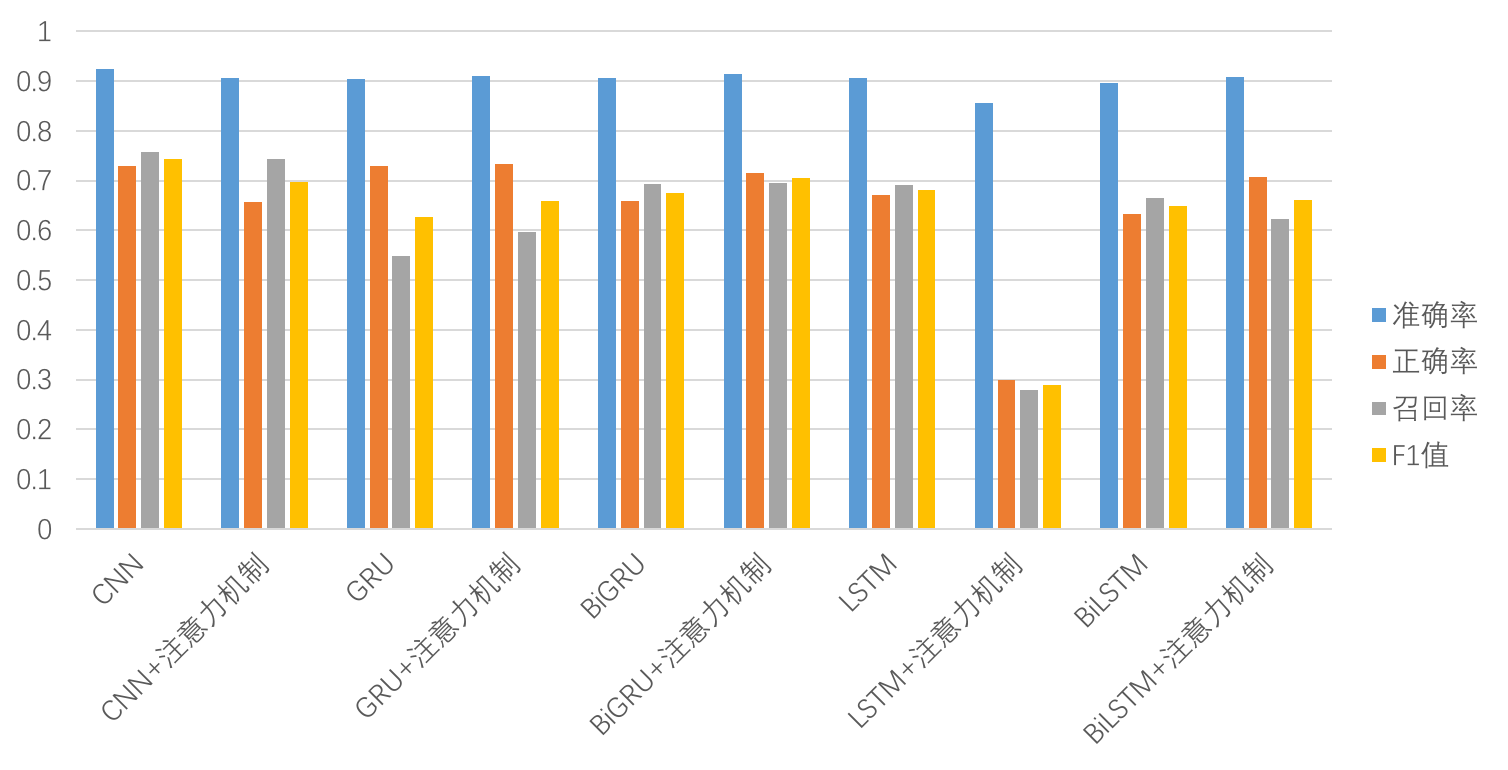
\includegraphics[width=\textwidth]{img/exp_context_emo_0_result_bar.png}
  \caption{面向情感四分类器的模型性能}
  \label{fig:exp_context_emo_0_result_bar}
\end{figure}

\subsubsection{面向“开心”、“悲伤”和“愤怒”三分类的模型性能分析}
\label{sssec:exp_context_emo_tri_base}

对于面向三轮对话的“开心”、“悲伤”和“愤怒”三分类问题,表~\ref{tab:exp_context_emo_tri_result}和图~\ref{fig:exp_context_emo_tri_result_bar}显示各个模型在测试集上的性能。注意表中的正确率、召回率、F1值同样对应章节~\ref{ssec:exp_context_emo_eval_metric}中定义的$P_\mu$、$R_\mu$和$F_\mu$。

对于表中的四个指标,均由CNN达到最好的效果。对于F1值,排第二和第三的分别是CNN配合注意力机制以及GRU配合注意力机制,两者和CNN的F1值差距明显(约0.0179)。对于准确率,第二的GRU配合注意力机制和第三的CNN配合注意力机制的数值接近,但都和CNN有一定差距(约0.132)。对于正确率,第二为CNN配合注意力机制,数值明显低于CNN(差距约0.0102)。对于召回率,由GRU配合注意力机制、BiGRU配合注意力机制、BiLSTM配合注意力机制并排第二,与CNN的召回率差距明显(约0.0219)。

另外,虽然添加注意力机制对CNN的性能依然没有正面作用,但GRU、BiGRU和BiLSTM在添加注意力机制后都有较明显的提升,显示注意力模型有效捕捉此问题背后的某种语言特征。

\begin{table}[htb]
  \centering
  \begin{minipage}[t]{\linewidth}
  \caption{面向“开心”、“悲伤”和“愤怒”的三分类器模型性能}
  \label{tab:exp_context_emo_tri_result}
    \begin{tabularx}{\linewidth}{X|llll}
    \toprule[1.5pt]
    & 准确率 & 正确率 & 召回率 & F1值 \\
    \hline
    CNN & \bf 0.9507 (1) & \bf 0.9454 (1) & \bf 0.9471 (1) & \bf 0.9462 (1) \\ % f_tri_cnn_ek_1554620372
    CNN+注意力机制 & 0.9351 (3) & 0.9352 (2) & 0.9215 (5) & 0.9283 (2) \\ % f_tri_cnn_ek_1554620395
    \hline
    GRU & 0.9315 (6) & 0.9278 (4) & 0.9142 (9) & 0.9210 (6) \\ % f_tri_gru_ek_1554576049
    GRU+注意力机制 & 0.9375 (2) & 0.9303 (3) & 0.9252 (2) & 0.9277 (3) \\ % f_tri_gru_ek_1554612493
    \hline
    BiGRU & 0.9303 (7) & 0.9212 (8) & 0.9179 (7) & 0.9196 (8) \\ % f_tri_bgru_ek_1554576063
    BiGRU+注意力机制 & 0.9339 (4) & 0.9235 (6) & 0.9252 (2) & 0.9243 (5) \\ % f_tri_bgru_ek_1554612494
    \hline
    LSTM & 0.9291 (8) & 0.9229 (7) & 0.9179 (7) & 0.9204 (7) \\ % f_tri_lstm_ek_1554575910
    LSTM+注意力机制 & 0.9279 (9) & 0.9180 (9) & 0.9197 (6) & 0.9189 (9) \\ % f_tri_lstm_ek_1554612497
    \hline
    BiLSTM & 0.9279 (9) & 0.9176 (10) & 0.9142 (9) & 0.9159 (10) \\ % f_tri_blstm_ek_1554575896
    BiLSTM+注意力机制 & 0.9339 (4) & 0.9269 (5) & 0.9252 (2) & 0.9260 (4) \\ % f_tri_blstm_ek_1554612490
    \bottomrule[1.5pt]
    \end{tabularx}
  \end{minipage}
\end{table}

\begin{figure}[H]
  \centering
  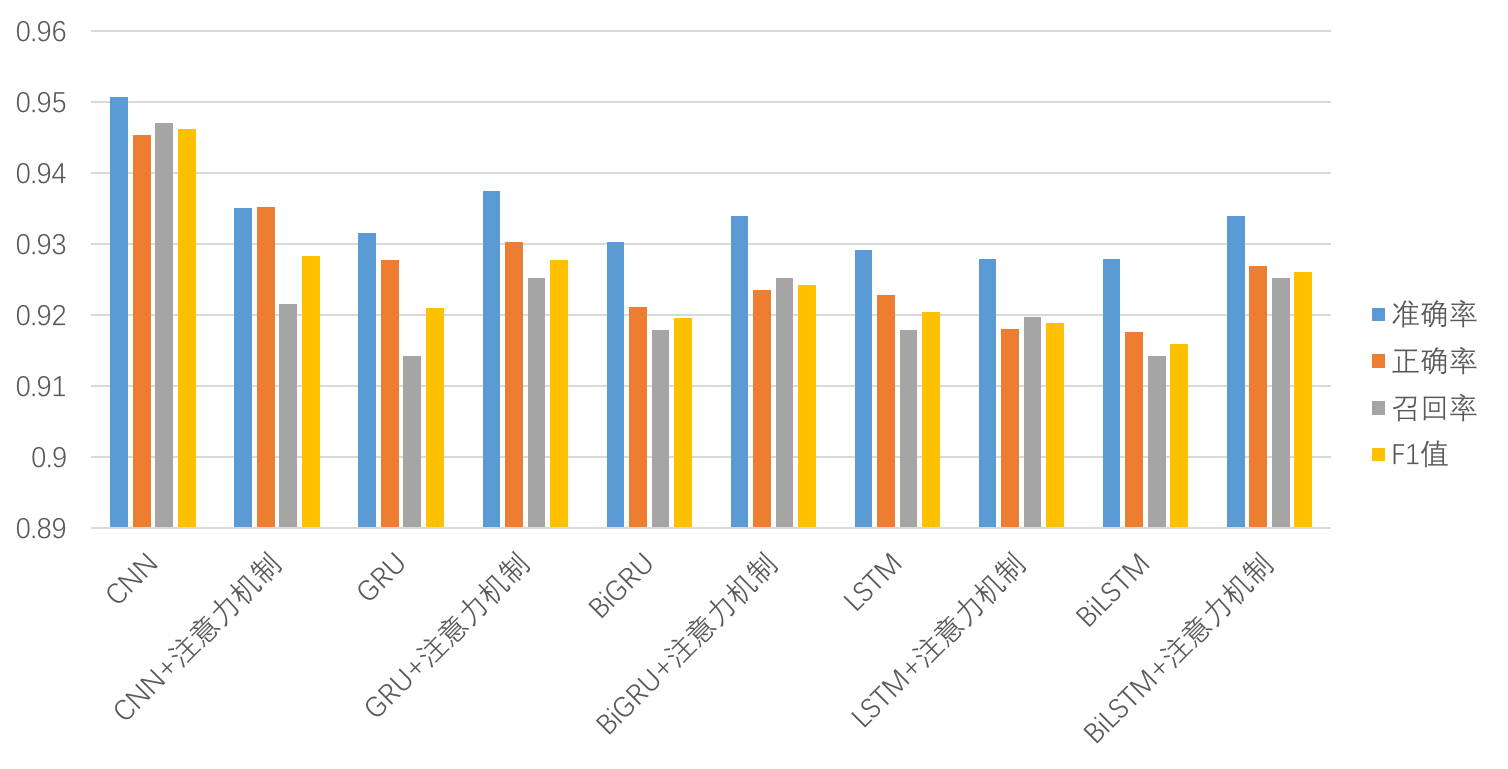
\includegraphics[width=\textwidth]{img/exp_context_emo_tri_result_bar.png}
  \caption{面向“开心”、“悲伤”和“愤怒”的三分类器模型性能}
  \label{fig:exp_context_emo_tri_result_bar}
\end{figure}

\subsubsection{面向“其他”和“不是其他”二分类的模型性能分析}
\label{sssec:exp_context_emo_b_base}

对于面向三轮对话的“其他”和“不是其他”二分类问题,表~\ref{tab:exp_context_emo_b_result}和图~\ref{fig:exp_context_emo_b_result_bar}显示各个模型在测试集上的性能。注意表中的正确率、召回率、F1值同样对应“其他”一类的指标。

对于F1值,GRU配合注意力机制达到最高数值的0.9546, 其次的CNN和BiGRU配合注意力机制
都和前者的数值接近(分别为0.9540和0.9494)。对于准确率,排名前三的模型同样依次是GRU配合注意力机制、CNN和BiGRU配合注意力机制,前两者数值比较接近(0.9230和0.9227),第三的数值(0.9152)则和前两者差距较明显。对于正确率,由GRU达到最好的性能(0.9670),其次的LSTM(0.9649)和CNN(0.9634)的性能也比较接近。 对于召回率,排名第一第二的依然是GRU配合注意力机制(0.9549)和CNN(0.9448),CNN配合注意力机制以及LSTM配合注意力机制并排第三(0.9391)。

虽然GRU配合注意力机制在三项指标上都排名第一,但其正确率却是各个模型中排名倒数第一。相对地,对正确率排名第一第二的LSTM和GRU,它们在另外三项指标上却都排名倒数第一第二。可见数据不均匀会影响模型的识别倾向,甚至出现模型只在个别指标上明显靠前但同时也其他指标上明显靠后的情况。

\begin{table}[htb]
  \centering
  \begin{minipage}[t]{\linewidth}
  \caption{面向“其他”和“不是其他”的二分类模型性能}
  \label{tab:exp_context_emo_b_result}
    \begin{tabularx}{\linewidth}{X|llll}
    \toprule[1.5pt]
    & 准确率 & 正确率 & 召回率 & F1值 \\
    \hline
    CNN & 0.9227 (2) & 0.9634 (3) & 0.9448 (2) & 0.9540 (2) \\ % f_b_cnn_ek_1554620963 
    CNN+注意力机制 & 0.9116 (7) & 0.9560 (9) & 0.9391 (3) & 0.9475 (7) \\ % f_b_cnn_ek_1554620537 
    \hline
    GRU & 0.9074 (9) & \bf 0.9670 (1) & 0.9224 (9) & 0.9442 (9) \\ % f_b_gru_ek_1554547645 
    GRU+注意力机制 & \bf 0.9230 (1) & 0.9553 (10) & \bf 0.9540 (1) & \bf 0.9546 (1) \\ % f_b_gru_ek_1554561028 
    \hline
    BiGRU & 0.9134 (4) & 0.9630 (4) & 0.9339 (6) & 0.9482 (4) \\ % f_b_bgru_ek_1554547845 
    BiGRU+注意力机制 & 0.9152 (3) & 0.9624 (6) & 0.9367 (5) & 0.9494 (3) \\ % f_b_bgru_ek_1554561013 
    \hline
    LSTM & 0.9011 (10) & 0.9649 (2) & 0.9168 (10) & 0.9402 (10) \\ % f_b_lstm_ek_1554549276 
    LSTM+注意力机制 & 0.9121 (6) & 0.9567 (8) & 0.9391 (3) & 0.9478 (6) \\ % f_b_lstm_ek_1554554626 
    \hline
    BiLSTM & 0.9089 (8) & 0.9595 (7) & 0.9320 (8) & 0.9456 (8) \\ % f_b_blstm_ek_1554549287 
    BiLSTM+注意力机制 & 0.9131 (5) & 0.9627 (5) & 0.9337 (7) & 0.9480 (5) \\ % f_b_blstm_ek_1554553473 
    \bottomrule[1.5pt]
    \end{tabularx}
  \end{minipage}
\end{table}

\begin{figure}[H]
  \centering
  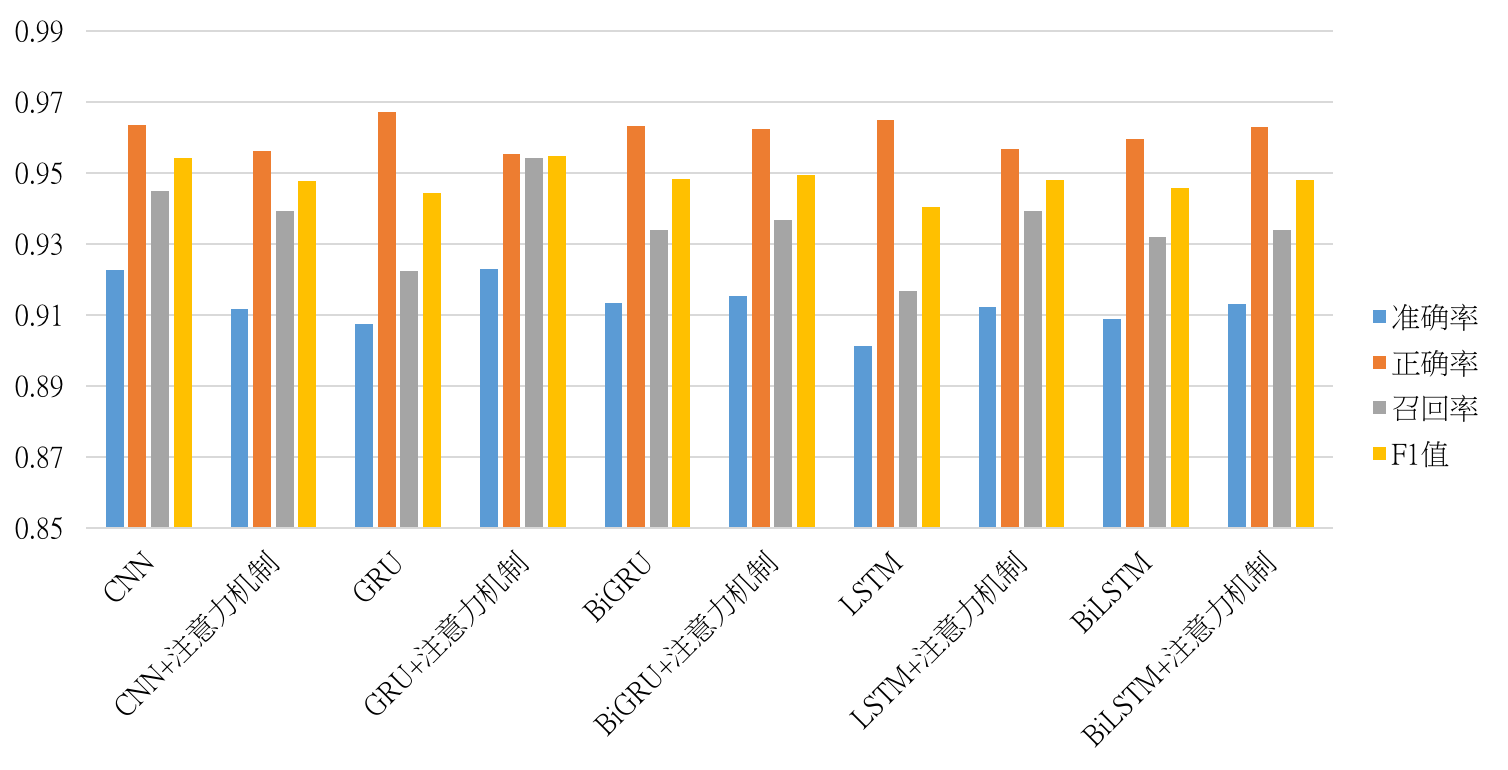
\includegraphics[width=\textwidth]{img/exp_context_emo_b_result_bar.png}
  \caption{面向“其他”和“不是其他”的二分类模型性能}
  \label{fig:exp_context_emo_b_result_bar}
\end{figure}

\subsubsection{面向三轮对话的情感识别系统的性能分析}

经过前面各章节的分析,我们已经对各个子分类问题中不同模型的性能有大致了解,接下来我们将研究由多组子分类器集成得出的情感识别系统的性能,并和比赛SemEval-2019任务三的参赛系统比较来评估我们系统的性能水平。

按照章节~\ref{sec:exp_context_emo_framework},我们的情感识别算法涉及三个子分类问题。对于和原问题相同的情感四分类问题,根据章节~\ref{sssec:exp_context_emo_0_base}的实验结果,我们采用CNN作为第一组分类器的模型。对于面向“开心”、“悲伤”和“愤怒”的三分类问题,按照章节~\ref{sssec:exp_context_emo_tri_base}的实验结果,我们同样选用CNN作为第二组分类器的模型。对于面向“其他”和“不是其他”的二分类问题,按照章节~\ref{sssec:exp_context_emo_b_base}的实验结果,我们采用GRU作为第三组分类器的模型。按照章节~\ref{ssec:exp_context_emo_model_training},我们基于选定的模型分别为每个分类器组训练5个分类器。

最后按照章节~\ref{sec:exp_context_emo_framework}中给出的识别流程,透过逐步结合各组分类器的投票结果得出三轮对话中最后一轮所表达的情感类别。对于系统中对第二、三组分类器需要配置的参数$thr_2$和$thr_3$,我们均设置为3。

表~\ref{tab:exp_context_emo_other_comp}显示我们的系统和SemEval-2019任务三中其他参赛系统在测试集上最后一次提交的性能。注意表中的F1值为
针对“开心”、“悲伤”和“愤怒”的指标,即章节~\ref{ssec:exp_context_emo_eval_metric}中定义的$F_\mu$。在SemEval-2019任务三的最终测试阶段,参赛系统共165个,但官方只给出了各个参赛系统的F1值。表中仅显示排名前10(按照F1值排名)的参赛系统,其中队伍名称为THU\_HCSI对应我们当时提交的系统,排名第8。

\begin{table}[htb]
  \centering
  \begin{minipage}[t]{0.6\linewidth}
  \caption{SemEval-2019任务三前十名参赛系统性能} % 总参赛队伍165
  \label{tab:exp_context_emo_other_comp}
    \begin{tabularx}{\linewidth}{c|X|c}
    \toprule[1.5pt]
    排名 & 队伍名称 & F1值 \\
    \hline
    1 & PingAn GammaLab & 0.7959 \\
    2 & (无) & 0.7947 \\
    3 & NELEC & 0.7765 \\
    4 & SymantoResearch & 0.7731 \\
    5 & ANA & 0.7709 \\
    6 & CAiRE\_HKUST & 0.7677 \\
    7 & SNU\_IDS & 0.7661 \\
    8 & \bf THU\_HCSI & 0.7616 \\
    9 & (无) & 0.7608 \\
    10 & YUN-HPCC & 0.7588 \\
    \bottomrule[1.5pt]
    \end{tabularx}
  \end{minipage}
\end{table}

另外,由于我们的算法中每一步的输出都可以作为一组预测结果,因此我们观察了每个中间结果在测试集上的性能。以下的系统由重新训练的子分类器组成,由于子分类器的训练存在随机性(参考章节~\ref{ssec:exp_context_emo_model_training}),因此和我们当时的参赛系统的F1值不同,但并不影响我们分析系统中每步决策的作用。

\begin{table}[htb]
  \centering
  \begin{minipage}[t]{0.6\linewidth}
  \caption{多分类器分层识别算法的中间结果和最终结果在测试集上的性能}
  \label{tab:exp_context_emo_ensemble_result}
    \begin{tabularx}{\linewidth}{X|cccc}
    \toprule[1.5pt]
    & 准确率 & 正确率 & 召回率 & F1值 \\
    \hline
    中间结果I & 0.9278 & 0.7360 & 0.7740 & 0.7545 \\
    中间结果II & 0.9281 & 0.7383 & \bf 0.7764 & 0.7569 \\
    \hline
    最终结果 & \bf 0.9299 & \bf 0.7474 & 0.7752 & \bf 0.7611 \\ 
    \bottomrule[1.5pt]
    \end{tabularx}
  \end{minipage}
\end{table}

表~\ref{tab:exp_context_emo_ensemble_result}中第一行“中间结果I”对应直接由一组情感四分类器(第一组分类器)进行多数投票的识别结果。第二行“中间结果II”是基于“开心”、“悲伤”和“愤怒”三分类器组(第二组分类器)的投票对原本被识别为这三个类别之一的样本重新进行分类的识别结果,可见四项指标都有所提升。再对比中间结果I和中间结果II的混淆矩阵(分别对应表~\ref{tab:exp_context_emo_conf_mat_1}和表~\ref{tab:exp_context_emo_conf_mat_2})可以发现4个样本的识别结果被正确修正,2个“愤怒”的样本被误判为“悲伤”,这显示了即使引入阈值$thr_2$来评估投票的可信度,由子分类器之间投票得出的识别结果依然会存在判断出错的情况,但整体上还是加强了对“开心”、“悲伤”和“愤怒”的区分能力。

表中最底一行的“最终结果”是基于“其他”和“不是其他”的二分类器组(第三组分类器)的投票结果尝试召回更多“其他”的样本,可见除了召回率有稍微下降,其他三项指标都有所提升,虽然准确率只稍微上升,但正确率的明显提升大大提高了最终的F1值。再对比中间结果II和最终结果的混淆矩阵(分别对应表~\ref{tab:exp_context_emo_conf_mat_2}和表~\ref{tab:exp_context_emo_conf_mat_3})可以发现11个“其他”的样本被正确召回,间接提高了“开心”、“悲伤”和“愤怒”的正确率$P_\mu$,但同时误判了1个原本正确的样本,故召回率$R_\mu$下降。同样地第三组分类器在引入阈值$thr_3$后依然会为识别结果带来错误的修改,但被正确召回的样本比错误的多,整体上对系统的识别结果也是起着正面的作用。

接下来,我们分析一下选择面向“开心”、“悲伤”和“愤怒”三分类以及面向“其他”和“不是其他”二分类这两个子分类问题的合理性。首先对于面向“开心”、“悲伤”和“愤怒”的三分类问题,参考章节\ref{sssec:exp_context_emo_tri_base}可以发现我们的模型在该子问题上有很好的区分能力(F1值达到0.9462),其数值明显高于原本的四分类问题(对比章节\ref{sssec:exp_context_emo_0_base}中最高的F1值为0.7437),可见在引入类别“其他”后对F1值有较大影响,一方面是数据量的增加,另一方面说明模型同时区分“其他”和另外三个类别存在较明显的困难。另外,回顾章节\ref{sssec:exp_context_emo_0_base}、\ref{sssec:exp_context_emo_tri_base}和\ref{sssec:exp_context_emo_b_base}可以发现前两个子问题中F1值最高的都是CNN,而后者F1值最高的是GRU配合注意力机制,显示“其他”和另外三个类别背后的数学模型应该稍有不同。因此在第二步中我们以CNN重新对被识别为“开心”、“悲伤”和“愤怒”的样本进行区分,然后在第三步中以不同的模型来识别出原本没有被召回的“其他”的样本,以结合两种模型的识别能力。

对于为什么只召回“其他”的样本,而没有反过来召回“不是其他”的样本再进行三分类,这和各类别样本量的分布有关。“其他”的样本量在测试上明显多于另外三个类别的样本量,
如果尝试进一步召回“不是其他”的样本,系统会同时把更多“其他”的样本误判为“不是其他”,这就导致正确率$P_\mu$的下降显着大于召回率$R_\mu$的提升,从而导致核心指标$F_\mu$下降。而相反地从原本被识别为“开心”、“悲伤”和“愤怒”的样本中召回“其他”的样本,虽然会把部分原本识别正确的样本误判为“其他”,但会有较大概率召回更多正确的“其他”的样本,间接提高正确率$P_\mu$,因此我们选择召回更多“其他”的样本作为第三步的核心目标。

\begin{table}[]
  \centering
  \begin{minipage}[t]{0.54\linewidth}
  \caption{
    \label{tab:exp_context_emo_conf_mat_1}
    测试集上中间结果I对应的混淆矩阵
  }
  \begin{tabularx}{\linewidth}{c|c|cccc}
  \toprule[1.5pt]
  \multicolumn{2}{c|}{\multirow{2}{*}} & \multicolumn{4}{c}{预测标签}    \\
  \cline{3-6} 
  \multicolumn{2}{c|}{}
    & 其他 & 开心 & 悲伤 & 愤怒  \\
  \hline
  \multirow{4}{*}{真实标签}
    & 其他 & 4467 & 65 & 57 & 88 \\
    & 开心 & 82 & 196 & 4 & 2 \\
    & 悲伤 & 38 & 2 & 201 & 9 \\
    & 愤怒 & 47 & 1 & 3 & 247 \\
  \bottomrule[1.5pt]
  \end{tabularx}
  \end{minipage}
\end{table}

\begin{table}[]
  \centering
  \begin{minipage}[t]{0.54\linewidth}
  \caption{
    \label{tab:exp_context_emo_conf_mat_2}
    测试集上中间结果II对应的混淆矩阵
  }
  \begin{tabularx}{\linewidth}{c|c|cccc}
  \toprule[1.5pt]
  \multicolumn{2}{c|}{\multirow{2}{*}} & \multicolumn{4}{c}{预测标签}    \\
  \cline{3-6} 
  \multicolumn{2}{c|}{}
    & 其他 & 开心 & 悲伤 & 愤怒  \\
  \hline
  \multirow{4}{*}{真实标签}
    & 其他 & 4467 & 65 & 60 & 85 \\
    & 开心 & 82 & 197 & 4 & 1 \\
    & 悲伤 & 38 & 1 & 204 & 7 \\
    & 愤怒 & 47 & 1 & 5 & 245 \\
  \bottomrule[1.5pt]
  \end{tabularx}
  \end{minipage}
\end{table}

\begin{table}[]
  \centering
  \begin{minipage}[t]{0.54\linewidth}
  \caption{
    \label{tab:exp_context_emo_conf_mat_3}
    测试集上最终结果对应的混淆矩阵
  }
  \begin{tabularx}{\linewidth}{c|c|cccc}
  \toprule[1.5pt]
  \multicolumn{2}{c|}{\multirow{2}{*}} & \multicolumn{4}{c}{预测标签}    \\
  \cline{3-6} 
  \multicolumn{2}{c|}{}
    & 其他 & 开心 & 悲伤 & 愤怒  \\
  \hline
  \multirow{4}{*}{真实标签}
    & 其他 & 4478 & 60 & 57 & 82 \\
    & 开心 & 82 & 197 & 4 & 1 \\
    & 悲伤 & 39 & 1 & 203 & 7 \\
    & 愤怒 & 47 & 1 & 5 & 245 \\
  \bottomrule[1.5pt]
  \end{tabularx}
  \end{minipage}
\end{table}

\subsection{错误分析}
\label{ssec:exp_context_emo_error_analysis}

本节中,我们将对系统错误识别的样本进行观察,分析其中的原因,从而对问题有更探入的了解,以及尝试给出下一步的改进方向。以下使用的例子均参照表~\ref{tab:semeval_2019_task3_error}。

\begin{table}[]
  \centering
  \begin{minipage}[t]{0.7\linewidth}
  \caption{
    \label{tab:semeval_2019_task3_error}
    测试集中被系统误判的样本例子
  }
  \begin{tabularx}{\linewidth}{c|c|l}
  \toprule[1.5pt]

   编号 & 类别 & 对话    \\
  \hline
  \multirow{3}{*}{1} & \multirow{3}{*}{开心} 
    &   (第一轮)用户甲: I'm in mood \\
    & & (第二轮)用户乙: ya need a hug ? :-) \\
    & & (第三轮)用户甲: yeah \\
  \hline
  \multirow{3}{*}{2} & \multirow{3}{*}{悲伤} 
    &   (第一轮)用户甲: I am \\
    & & (第二轮)用户乙: in your dreams \\
    & & (第三轮)用户甲: Haha Bite me! 
\includegraphics[height=1.5\fontcharht\font`\B]{img/emoji/speechless.png}
\includegraphics[height=1.5\fontcharht\font`\B]{img/emoji/speechless.png}
\includegraphics[height=1.5\fontcharht\font`\B]{img/emoji/speechless.png} \\
  \hline
  \multirow{3}{*}{3} & \multirow{3}{*}{愤怒} 
    &   (第一轮)用户甲: You are pig \\
    & & (第二轮)用户乙: so are you \\
    & & (第三轮)用户甲: You are dog \\
  \hline
  \multirow{3}{*}{4} & \multirow{3}{*}{其他} 
    &   (第一轮)用户甲: Wat u wanna knw? \\
    & & (第二轮)用户乙: i knw nothin :P \\
    & & (第三轮)用户甲: 
\includegraphics[height=1.5\fontcharht\font`\B]{img/emoji/lol.png}
\includegraphics[height=1.5\fontcharht\font`\B]{img/emoji/lol.png} \\
  \hline
  \multirow{3}{*}{5} & \multirow{3}{*}{开心} 
    &   (第一轮)用户甲: You cannot see my hair \\
    & & (第二轮)用户乙: I'm in your closet \\
    & & (第三轮)用户甲: 
\includegraphics[height=1.5\fontcharht\font`\B]{img/emoji/lol.png} \\
  \bottomrule[1.5pt]
  \end{tabularx}
  \end{minipage}
\end{table}


\begin{itemize}

\item {\bf 词组情感倾向识别}。参考例子1,第一轮中用户甲的“in mood”表示心情愉快,属于正向情感,第三轮中的“yeah”也略带正向情感,按照章节~\ref{ssec:exp_context_emo_multi_turn_analyse},应该得出样本情感标签为“开心”。然而“in mood”在训练集中主要以“not in mood”出现,且这些样本标签都是“悲伤”,显然系统未能正确识别“in mood”本身的情感倾向导致了识别错误,另外可以推测对于在训练集上没有出现过的词组也会有相同的问题。在章节~\ref{ssec:exp_irony_det_error_analysis}中相同,只能透过额外引入语言知识解决。

\item {\bf 对于同时出现多种情感的处理}。参考例子2,第三轮中用户甲的发言在字面上包含两种情感,首先是“Haha”表达偏向“开心”的情感,“Bite me!
\includegraphics[height=1.5\fontcharht\font`\B]{img/emoji/speechless.png}”则带有鄙视和不满的意思,倾向于“悲伤”。按照章节~\ref{ssec:exp_context_emo_multi_turn_analyse}的分析,应以后半“悲伤”的情感为主。然而我们选用的CNN模型中,CNN的序列输出以最大池整合为一个固定长度的向量,即模型没有考虑情感出现的先后顺序,而是直接保留了字面上情感最强烈的内容,这也显示对语言模式的了解有助于模型的设计。

\item {\bf 理解比喻修辞}。参考例子3,用户甲在第一轮和第三轮中都在以比喻的修辞辱骂用户乙,然而系统从字面意思上未能识别出其情感倾向于“愤怒”。首先,在训练集上确实存在“be a pig”且大部分的标注都为“愤怒”,理论上机器学习算法可以学习出“be a pig”带有表达“愤怒”的性质。但数据中没有包含“be a dog”的样本,那么如果算法未能关联“pig”和“dog”就不可能识别出“be a pig”的情感属性。而从语言的角度来看,解决这个问题的本质是识别出比喻的使用,并且理解其真实想表达的意思,这就回归到上一章节中对修辞手法进行建模的问题。

\item {\bf 语料中情感标注的不一致}。参考例子4,第三轮中用户甲的发言仅包含两个大笑的表情符“
\includegraphics[height=1.5\fontcharht\font`\B]{img/emoji/lol.png}”,而前两轮的文本内容则偏向中性,我们有理由认为这个样本应该标记为“开心”,然而组织者给出的标注为“其他”。再参考例子5,第三轮中用户甲的发言同样仅包含大笑的表情符“
\includegraphics[height=1.5\fontcharht\font`\B]{img/emoji/lol.png}”,而前两轮的文本内容同样偏向中性,但标注为“开心”。假如我们对例子4的情感判断正确,那就说明数据集内部对情感标注的标准存在不一致,这一方面会对模型的学习造成混淆,另一方面也会对系统评估带来影响。

\end{itemize}

\section{本章小结}

在本章中我们提出了一种多通道分类模型,用于研究面向三轮对话的情感识别,以结合各轮发言的信息。基于该模型,我们同时提出了一个多分类器分层情感识别算法,并用于国际比赛SemEval-2019任务三的情感识别问题,参赛结果显示我们系统的性能在165个参赛系统中排名前十。以此比赛为基础,我们进一步观察了我们的多分类器分层情感识别算法的性能表现,透过对算法的中间结果进行分析,解释了我们算法中每一步对整个算法的作用,同时验证了我们的算法设计的合理性。最后我们对被系统错误识别的样本进行分析,指出系统的不足之处并给出对应的改进方向。



\chapter{总结和展望}
\label{cha:conclusion}

\section{论文工作总结}

随着互联网用户越来越习惯于在社交媒体上发言,对这些数据进行内容分析的价值逐渐受到重视,相关研究得以蓬勃发展,面向文本的情感识别研究就是其中之一。本硕士论文探索了该领域下的两个核心问题:数据不均匀在多分类问题中的影响、在算法建模中引入上下文信息。为了解决以上两个问题,我们分别提出了一种基于多步决策的多分类系统设计方法以及一种多通道分类模型。本论文的主要研究工作如下:

\begin{enumerate}

\item {\bf 基于多步决策的微博反讽识别}。我们首先对和情感识别紧密相关的反讽识别进行研究,并指出在真实场景中数据不均匀的问题,为此我們提出了一种基于多步決策的多分类系統设计方法,把原本的多分类問题拆解成多个子分类問题的疊加,再透过逐步回答每个子分类問题得出最终的反讽识別结果。我们基于国际比赛SemEval-2018任务三的两个子任务进行实验。对于其中的子任务一,即识別微博文本是否带有反讽的二分类问题,我們訓練了一組以2层BiLSTM作为模型的二分类器,再透过多投票得出识別结果。实验结果显示我们的系统达到了当时参赛系统中靠前的性能,并和我们当时参赛的系统对比有了明显的进步。对子任务二,即在子任务一的基礎上把反讽细分成三个类别后的四分类问题,基于我们提出的系统设计方法,我们给出了一个具体的基于多步决策的反讽识别系统。实验结果显示我们系统在主要评价指标F1值上显着优于当时参赛系统中的第一,而在其他几项指标上都达到了仅次于第一名的数值,验证了我们系统的性能。另外透过对系统中间结果进行观察,我们解釋了多步决策中每一步如何对系統的整体性能帶來貢献,同时验证了我們系統设计方法的合理性。

\item {\bf 基于多通道模型引入上下文的情感识别}。为了研究如何在情感识別中引入上下文,我們研究了面向三轮对话的情感识别,同时提出了一种多通道分类模型,以结合起不同作用的上下文。我們基于国际比赛SemEval-2019的任务三进行实验。首先透过对语料进行观察,我们分析了三轮对话中每轮发言对识别最后一轮情感的作用,以此提出了一个三通道模型,再结合前面提出的系統设计方法,我們给出了一个具体的基于多步决策的情感识别系统。参赛结果显示我们的系统在165个参赛系统中排名前十。另外透过对系统的中间结果进行分析,我們验证了系統中每步決策的有效性,同时证明了基于多步決策的系統设计方法通用于不同的多分类問题,但需要針对核心评价指标和各个类別的样本分布挑选合适的子分类問题。

\end{enumerate}

\section{未来工作展望}

面向文本的情感识别技术在实际应用中有明显的不足之处,相关研究依然存在很大的进步空间。特别是随着信息技术发展,文本的使用场景只会变得越来越复杂。总结第\ref{cha:exp_irony_det}章和第\ref{cha:exp_context_emo}章我们对系统的错误分析,我们为面向文本情感识别的后续工作给出以下建议:

\begin{enumerate}

\item {\bf 多模型融合}。在两个章节的实验中,我们都指出了基于现阶段主流的人工神经网络可能无法同时对多个类别的数据进行拟合,原因在于各个类别背后的语言特征有本质上的不同。尝试提出拟合能力更强的人工神经网络结构固然是前进方向之一,但我们同时鼓励采用较简单的模型对局部数据进行建模,再透过类似我们提出的多步决策框架来结合各个模型捕足到的信息,以此解决单个模型建模能力有限的问题。
。

\item {\bf 引入语义知识}。文本情感识别的核心难点之一在于语义。机器学习方法只能从训练数据中尝试学习词(组)的语义,但应用场景中往往会出现训练数据中没有出现过的词(组),导致算法无法理解其中的信息。为了处理这部分内容,我们建议引入更多额外的语义知识,以建立在训练数据中出现过和没有出现过的词(组)之间的联系。词嵌入方法虽然在原理上能关联语义相近的词,但从实验结果来看依然有不足之处(如无法处理上一词多义的情况),这些问题都有待进一步探索。

\item {\bf 引入语用知识}。文本情感识别的核心难点其二在于丰富多样的语用,譬如反讽和比喻等修辞手法。如果没有意识到发言者使用了特殊的修辞手法,单凭字面意思了解文本内容就有可能忽略甚至曲解发言者本身想表达的意思。而为了识别修辞的使用,本文中尝试采用多种人工神经网络模型进行建模,但在对系统进行错误分析时,我们会发现一些显而易见的模式未能被系统正确识别。对于这部分样本,最直观的做法是采用基于规则的方法。修辞手法的具体使用虽然多种多样,但根据语用知识我们可以总结出其中有限种模式。进一步地,有别于单纯基于规则的方法,我们建议结合基于规则的方法和机器学习方法,优先召回能被规则匹配的样本,再由机器学习方法识别难以由人工归纳出规则的样本,以此减轻人工设计规则的压力。

\end{enumerate}









%%% 其它部分
\backmatter

%% 本科生要这几个索引,研究生不要。选择性留下。
% 插图索引
\listoffigures
% 表格索引
\listoftables
% 公式索引
\listofequations


%% 参考文献
% 注意:至少需要引用一篇参考文献,否则下面两行可能引起编译错误。
% 如果不需要参考文献,请将下面两行删除或注释掉。
% 数字式引用
\bibliographystyle{thuthesis-numeric}
% 作者-年份式引用
% \bibliographystyle{thuthesis-author-year}
\bibliography{ref/refs}


%% 致谢
% 如果使用声明扫描页,将可选参数指定为扫描后的 PDF 文件名,例如:
% \begin{acknowledgement}[scan-statement.pdf]
\begin{acknowledgement}

衷心感谢导师徐明星副教授多年来对本人的指导和帮助,使我在研究生期间的三年受益匪浅。徐老师在科研问题上有独特的想法,对于我主要研究的自然语言处理领域,当很多研究都专注于采用更复杂的模型进行尝试时,徐老师强调从语言的本质入手,除了亲自翻查语言学的相关材料,还会向心理学的老师谈讨交流,这种对研究的热情和好奇心对我有很大的感染力。除了学术以外,徐老师还会有一些为人处事方面的教导,确实做到了授业与解惑。在此再次表示由衷的感谢。

另外感谢在读期间帮过我的各位老师和同学,因为有你们的帮助使得我读研的三年过得更顺利。感谢家人在背后的支持,让我没有顾虑远离家乡完成我的学业。最后感谢每一位和我非常亲密的好友,在我完全学业期间充满压力的时候,是你们的支持帮我度过了这些困难的时刻。

最后再次向以上的各位表示衷心的感谢。

% 在美国麻省理工学院化学系进行九个月的合作研究期间,承蒙 xxx 教授热心指导与帮助,不胜感激。感谢 xx 实验室主任 xx 教授,以及实验室全体老师和同学们的热情帮助和支持!本课题承蒙国家自然科学基金资助,特此致谢。

% 感谢 \LaTeX 和 \thuthesis\cite{thuthesis},帮我节省了不少时间。
\end{acknowledgement}


%% 附录
% \begin{appendix}
% \chapter{外文资料原文}
\label{cha:engorg}

\title{The title of the English paper}

\textbf{Abstract:} As one of the most widely used techniques in operations
research, \emph{ mathematical programming} is defined as a means of maximizing a
quantity known as \emph{bjective function}, subject to a set of constraints
represented by equations and inequalities. Some known subtopics of mathematical
programming are linear programming, nonlinear programming, multiobjective
programming, goal programming, dynamic programming, and multilevel
programming$^{[1]}$.

It is impossible to cover in a single chapter every concept of mathematical
programming. This chapter introduces only the basic concepts and techniques of
mathematical programming such that readers gain an understanding of them
throughout the book$^{[2,3]}$.


\section{Single-Objective Programming}
The general form of single-objective programming (SOP) is written
as follows,
\begin{equation}\tag*{(123)} % 如果附录中的公式不想让它出现在公式索引中,那就请
                             % 用 \tag*{xxxx}
\left\{\begin{array}{l}
\max \,\,f(x)\\[0.1 cm]
\mbox{subject to:} \\ [0.1 cm]
\qquad g_j(x)\le 0,\quad j=1,2,\cdots,p
\end{array}\right.
\end{equation}
which maximizes a real-valued function $f$ of
$x=(x_1,x_2,\cdots,x_n)$ subject to a set of constraints.

\newtheorem{mpdef}{Definition}[chapter]
\begin{mpdef}
In SOP, we call $x$ a decision vector, and
$x_1,x_2,\cdots,x_n$ decision variables. The function
$f$ is called the objective function. The set
\begin{equation}\tag*{(456)} % 这里同理,其它不再一一指定。
S=\left\{x\in\Re^n\bigm|g_j(x)\le 0,\,j=1,2,\cdots,p\right\}
\end{equation}
is called the feasible set. An element $x$ in $S$ is called a
feasible solution.
\end{mpdef}

\newtheorem{mpdefop}[mpdef]{Definition}
\begin{mpdefop}
A feasible solution $x^*$ is called the optimal
solution of SOP if and only if
\begin{equation}
f(x^*)\ge f(x)
\end{equation}
for any feasible solution $x$.
\end{mpdefop}

One of the outstanding contributions to mathematical programming was known as
the Kuhn-Tucker conditions\ref{eq:ktc}. In order to introduce them, let us give
some definitions. An inequality constraint $g_j(x)\le 0$ is said to be active at
a point $x^*$ if $g_j(x^*)=0$. A point $x^*$ satisfying $g_j(x^*)\le 0$ is said
to be regular if the gradient vectors $\nabla g_j(x)$ of all active constraints
are linearly independent.

Let $x^*$ be a regular point of the constraints of SOP and assume that all the
functions $f(x)$ and $g_j(x),j=1,2,\cdots,p$ are differentiable. If $x^*$ is a
local optimal solution, then there exist Lagrange multipliers
$\lambda_j,j=1,2,\cdots,p$ such that the following Kuhn-Tucker conditions hold,
\begin{equation}
\label{eq:ktc}
\left\{\begin{array}{l}
    \nabla f(x^*)-\sum\limits_{j=1}^p\lambda_j\nabla g_j(x^*)=0\\[0.3cm]
    \lambda_jg_j(x^*)=0,\quad j=1,2,\cdots,p\\[0.2cm]
    \lambda_j\ge 0,\quad j=1,2,\cdots,p.
\end{array}\right.
\end{equation}
If all the functions $f(x)$ and $g_j(x),j=1,2,\cdots,p$ are convex and
differentiable, and the point $x^*$ satisfies the Kuhn-Tucker conditions
(\ref{eq:ktc}), then it has been proved that the point $x^*$ is a global optimal
solution of SOP.

\subsection{Linear Programming}
\label{sec:lp}

If the functions $f(x),g_j(x),j=1,2,\cdots,p$ are all linear, then SOP is called
a {\em linear programming}.

The feasible set of linear is always convex. A point $x$ is called an extreme
point of convex set $S$ if $x\in S$ and $x$ cannot be expressed as a convex
combination of two points in $S$. It has been shown that the optimal solution to
linear programming corresponds to an extreme point of its feasible set provided
that the feasible set $S$ is bounded. This fact is the basis of the {\em simplex
  algorithm} which was developed by Dantzig as a very efficient method for
solving linear programming.
\begin{table}[ht]
\centering
  \centering
  \caption*{Table~1\hskip1em This is an example for manually numbered table, which
    would not appear in the list of tables}
  \label{tab:badtabular2}
  \begin{tabular}[c]{|m{1.5cm}|c|c|c|c|c|c|}\hline
    \multicolumn{2}{|c|}{Network Topology} & \# of nodes &
    \multicolumn{3}{c|}{\# of clients} & Server \\\hline
    GT-ITM & Waxman Transit-Stub & 600 &
    \multirow{2}{2em}{2\%}&
    \multirow{2}{2em}{10\%}&
    \multirow{2}{2em}{50\%}&
    \multirow{2}{1.2in}{Max. Connectivity}\\\cline{1-3}
    \multicolumn{2}{|c|}{Inet-2.1} & 6000 & & & &\\\hline
    \multirow{2}{1.5cm}{Xue} & Rui  & Ni &\multicolumn{4}{c|}{\multirow{2}*{\thuthesis}}\\\cline{2-3}
    & \multicolumn{2}{c|}{ABCDEF} &\multicolumn{4}{c|}{} \\\hline
\end{tabular}
\end{table}

Roughly speaking, the simplex algorithm examines only the extreme points of the
feasible set, rather than all feasible points. At first, the simplex algorithm
selects an extreme point as the initial point. The successive extreme point is
selected so as to improve the objective function value. The procedure is
repeated until no improvement in objective function value can be made. The last
extreme point is the optimal solution.

\subsection{Nonlinear Programming}

If at least one of the functions $f(x),g_j(x),j=1,2,\cdots,p$ is nonlinear, then
SOP is called a {\em nonlinear programming}.

A large number of classical optimization methods have been developed to treat
special-structural nonlinear programming based on the mathematical theory
concerned with analyzing the structure of problems.
\begin{figure}[h]
  \centering
  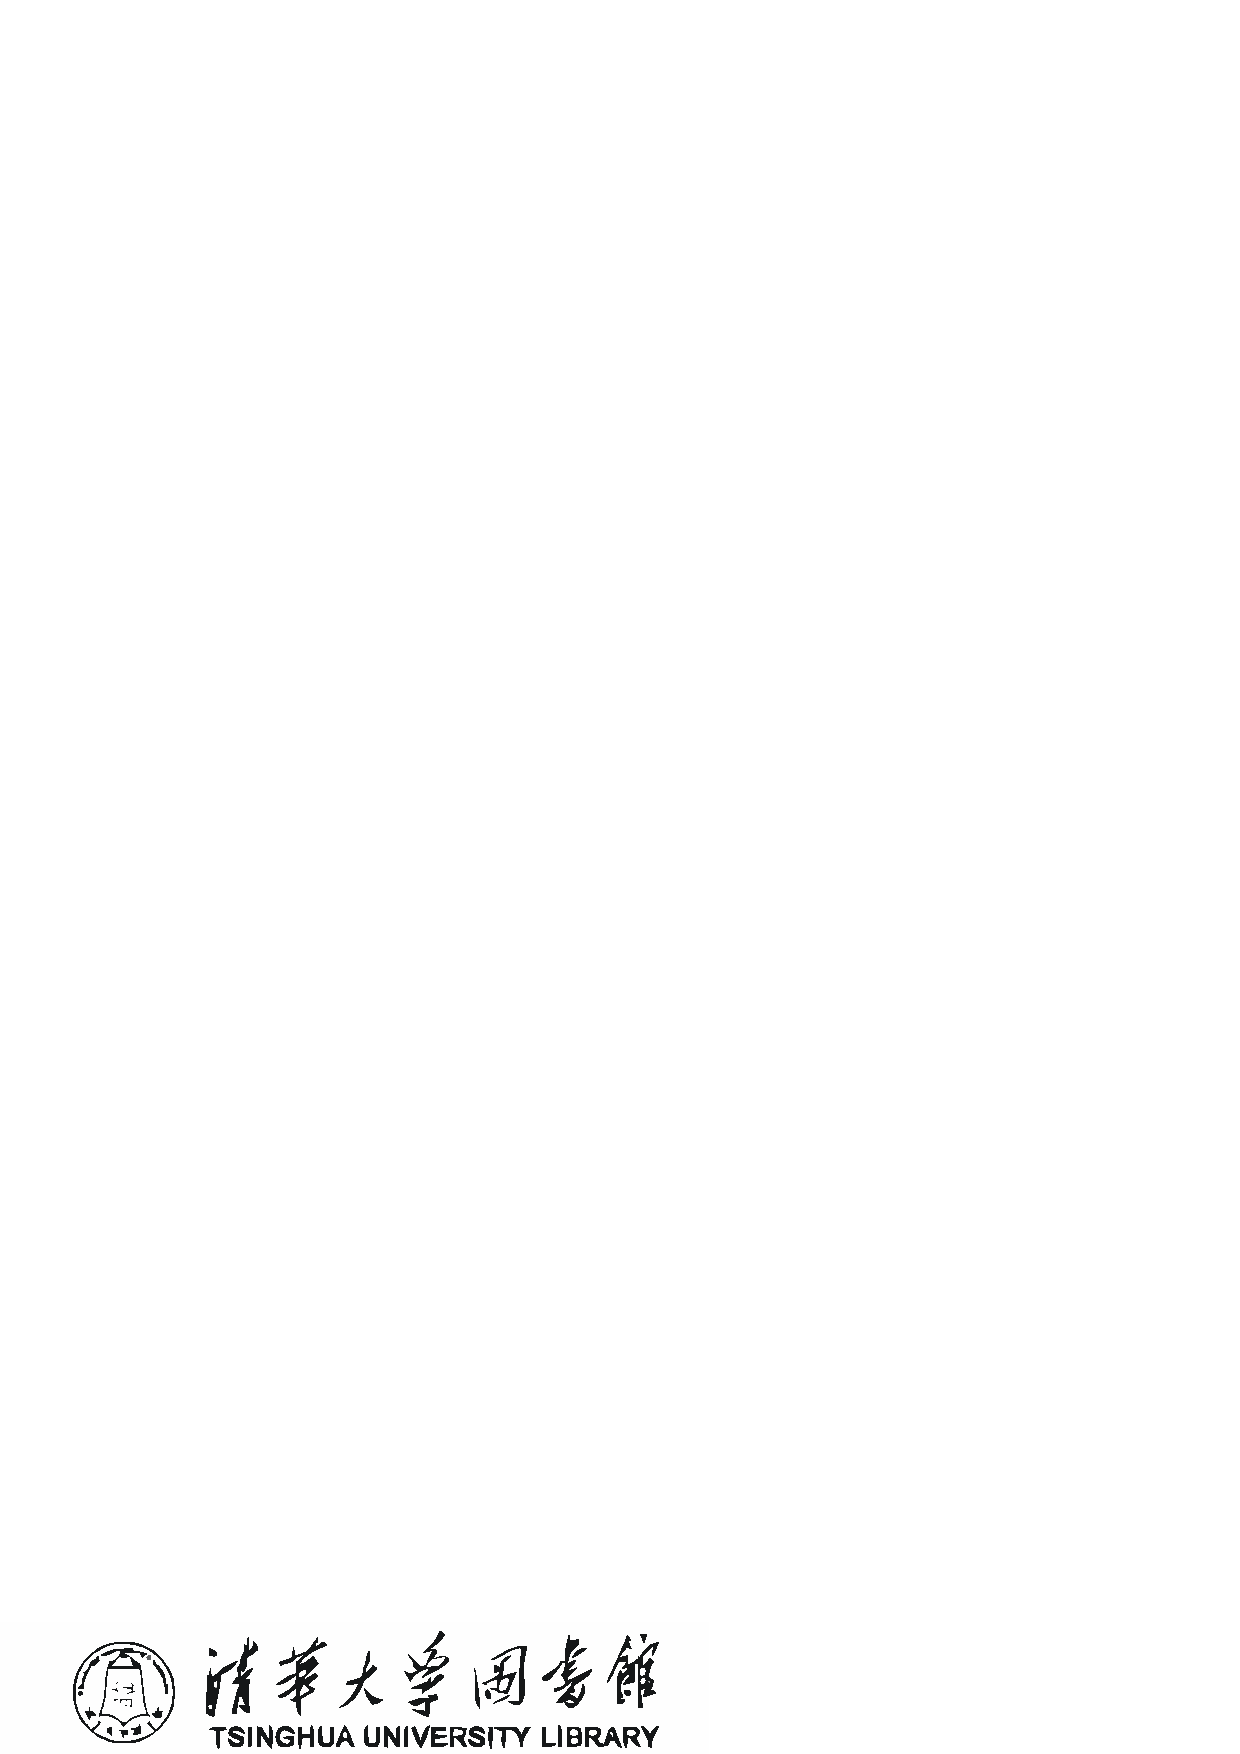
\includegraphics{thu-lib-logo}
  \caption*{Figure~1\quad This is an example for manually numbered figure,
    which would not appear in the list of figures}
  \label{tab:badfigure2}
\end{figure}

Now we consider a nonlinear programming which is confronted solely with
maximizing a real-valued function with domain $\Re^n$.  Whether derivatives are
available or not, the usual strategy is first to select a point in $\Re^n$ which
is thought to be the most likely place where the maximum exists. If there is no
information available on which to base such a selection, a point is chosen at
random. From this first point an attempt is made to construct a sequence of
points, each of which yields an improved objective function value over its
predecessor. The next point to be added to the sequence is chosen by analyzing
the behavior of the function at the previous points. This construction continues
until some termination criterion is met. Methods based upon this strategy are
called {\em ascent methods}, which can be classified as {\em direct methods},
{\em gradient methods}, and {\em Hessian methods} according to the information
about the behavior of objective function $f$. Direct methods require only that
the function can be evaluated at each point. Gradient methods require the
evaluation of first derivatives of $f$. Hessian methods require the evaluation
of second derivatives. In fact, there is no superior method for all
problems. The efficiency of a method is very much dependent upon the objective
function.

\subsection{Integer Programming}

{\em Integer programming} is a special mathematical programming in which all of
the variables are assumed to be only integer values. When there are not only
integer variables but also conventional continuous variables, we call it {\em
  mixed integer programming}. If all the variables are assumed either 0 or 1,
then the problem is termed a {\em zero-one programming}. Although integer
programming can be solved by an {\em exhaustive enumeration} theoretically, it
is impractical to solve realistically sized integer programming problems. The
most successful algorithm so far found to solve integer programming is called
the {\em branch-and-bound enumeration} developed by Balas (1965) and Dakin
(1965). The other technique to integer programming is the {\em cutting plane
  method} developed by Gomory (1959).

\hfill\textit{Uncertain Programming\/}\quad(\textsl{BaoDing Liu, 2006.2})

\section*{References}
\noindent{\itshape NOTE: These references are only for demonstration. They are
  not real citations in the original text.}

\begin{translationbib}
\item Donald E. Knuth. The \TeX book. Addison-Wesley, 1984. ISBN: 0-201-13448-9
\item Paul W. Abrahams, Karl Berry and Kathryn A. Hargreaves. \TeX\ for the
  Impatient. Addison-Wesley, 1990. ISBN: 0-201-51375-7
\item David Salomon. The advanced \TeX book.  New York : Springer, 1995. ISBN:0-387-94556-3
\end{translationbib}

\chapter{外文资料的调研阅读报告或书面翻译}

\title{英文资料的中文标题}

{\heiti 摘要:} 本章为外文资料翻译内容。如果有摘要可以直接写上来,这部分好像没有
明确的规定。

\section{单目标规划}
北冥有鱼,其名为鲲。鲲之大,不知其几千里也。化而为鸟,其名为鹏。鹏之背,不知其几
千里也。怒而飞,其翼若垂天之云。是鸟也,海运则将徙于南冥。南冥者,天池也。
\begin{equation}\tag*{(123)}
 p(y|\mathbf{x}) = \frac{p(\mathbf{x},y)}{p(\mathbf{x})}=
\frac{p(\mathbf{x}|y)p(y)}{p(\mathbf{x})}
\end{equation}

吾生也有涯,而知也无涯。以有涯随无涯,殆已!已而为知者,殆而已矣!为善无近名,为
恶无近刑,缘督以为经,可以保身,可以全生,可以养亲,可以尽年。

\subsection{线性规划}
庖丁为文惠君解牛,手之所触,肩之所倚,足之所履,膝之所倚,砉然响然,奏刀騞然,莫
不中音,合于桑林之舞,乃中经首之会。
\begin{table}[ht]
\centering
  \centering
  \caption*{表~1\hskip1em 这是手动编号但不出现在索引中的一个表格例子}
  \label{tab:badtabular3}
  \begin{tabular}[c]{|m{1.5cm}|c|c|c|c|c|c|}\hline
    \multicolumn{2}{|c|}{Network Topology} & \# of nodes &
    \multicolumn{3}{c|}{\# of clients} & Server \\\hline
    GT-ITM & Waxman Transit-Stub & 600 &
    \multirow{2}{2em}{2\%}&
    \multirow{2}{2em}{10\%}&
    \multirow{2}{2em}{50\%}&
    \multirow{2}{1.2in}{Max. Connectivity}\\\cline{1-3}
    \multicolumn{2}{|c|}{Inet-2.1} & 6000 & & & &\\\hline
    \multirow{2}{1.5cm}{Xue} & Rui  & Ni &\multicolumn{4}{c|}{\multirow{2}*{\thuthesis}}\\\cline{2-3}
    & \multicolumn{2}{c|}{ABCDEF} &\multicolumn{4}{c|}{} \\\hline
\end{tabular}
\end{table}

文惠君曰:“嘻,善哉!技盖至此乎?”庖丁释刀对曰:“臣之所好者道也,进乎技矣。始臣之
解牛之时,所见无非全牛者;三年之后,未尝见全牛也;方今之时,臣以神遇而不以目视,
官知止而神欲行。依乎天理,批大郤,导大窾,因其固然。技经肯綮之未尝,而况大坬乎!
良庖岁更刀,割也;族庖月更刀,折也;今臣之刀十九年矣,所解数千牛矣,而刀刃若新发
于硎。彼节者有间而刀刃者无厚,以无厚入有间,恢恢乎其于游刃必有余地矣。是以十九年
而刀刃若新发于硎。虽然,每至于族,吾见其难为,怵然为戒,视为止,行为迟,动刀甚微,
謋然已解,如土委地。提刀而立,为之而四顾,为之踌躇满志,善刀而藏之。”

文惠君曰:“善哉!吾闻庖丁之言,得养生焉。”


\subsection{非线性规划}
孔子与柳下季为友,柳下季之弟名曰盗跖。盗跖从卒九千人,横行天下,侵暴诸侯。穴室枢
户,驱人牛马,取人妇女。贪得忘亲,不顾父母兄弟,不祭先祖。所过之邑,大国守城,小
国入保,万民苦之。孔子谓柳下季曰:“夫为人父者,必能诏其子;为人兄者,必能教其弟。
若父不能诏其子,兄不能教其弟,则无贵父子兄弟之亲矣。今先生,世之才士也,弟为盗
跖,为天下害,而弗能教也,丘窃为先生羞之。丘请为先生往说之。”
\begin{figure}[h]
  \centering
  
\includegraphics{thu-whole-logo}
  \caption*{图~1\hskip1em 这是手动编号但不出现索引中的图片的例子}
  \label{tab:badfigure3}
\end{figure}

柳下季曰:“先生言为人父者必能诏其子,为人兄者必能教其弟,若子不听父之诏,弟不受
兄之教,虽今先生之辩,将奈之何哉?且跖之为人也,心如涌泉,意如飘风,强足以距敌,
辩足以饰非。顺其心则喜,逆其心则怒,易辱人以言。先生必无往。”

孔子不听,颜回为驭,子贡为右,往见盗跖。

\subsection{整数规划}
盗跖乃方休卒徒大山之阳,脍人肝而餔之。孔子下车而前,见谒者曰:“鲁人孔丘,闻将军
高义,敬再拜谒者。”谒者入通。盗跖闻之大怒,目如明星,发上指冠,曰:“此夫鲁国之
巧伪人孔丘非邪?为我告之:尔作言造语,妄称文、武,冠枝木之冠,带死牛之胁,多辞缪
说,不耕而食,不织而衣,摇唇鼓舌,擅生是非,以迷天下之主,使天下学士不反其本,妄
作孝弟,而侥幸于封侯富贵者也。子之罪大极重,疾走归!不然,我将以子肝益昼餔之膳。”


\chapter{其它附录}
前面两个附录主要是给本科生做例子。其它附录的内容可以放到这里,当然如果你愿意,可
以把这部分也放到独立的文件中,然后将其 \cs{input} 到主文件中。

% \end{appendix}

%% 个人简历
\begin{resume}

  \resumeitem{个人简历}

  1994 年 6 月 4 日出生于 澳门特别行政区。

  2012 年 9 月考入清华大学计算机科学与技术系,2016 年 7 月本科毕业并获得工学学士学位。

  2016 年 9 月免试进入清华大学计算机科学与技术系攻读硕士学位至今。

  \researchitem{发表的学术论文} % 发表的和录用的合在一起

  % 1. 已经刊载的学术论文(本人是第一作者,或者导师为第一作者本人是第二作者)
  % \begin{publications}
    % \item Yang Y, Ren T L, Zhang L T, et al. Miniature microphone with silicon-based ferroelectric thin films. Integrated Ferroelectrics, 2003, 52:229-235. (SCI 收录, 检索号:758FZ.)
    % \item 杨轶, 张宁欣, 任天令, 等. 硅基铁电微声学器件中薄膜残余应力的研究. 中国机械工程, 2005, 16(14):1289-1291. (EI 收录, 检索号:0534931 2907.)
    % \item 杨轶, 张宁欣, 任天令, 等. 集成铁电器件中的关键工艺研究. 仪器仪表学报, 2003, 24(S4):192-193. (EI 源刊.)
  % \end{publications}

  % 2. 尚未刊载,但已经接到正式录用函的学术论文(本人为第一作者,或者
  %    导师为第一作者本人是第二作者)。
  \begin{publications}[before=\publicationskip,after=\publicationskip]
    % \item Yang Y, Ren T L, Zhu Y P, et al. PMUTs for handwriting recognition. In press. (已被 Integrated Ferroelectrics 录用. SCI 源刊.)

    \item Xihao Liang, Ye Ma, Mingxing Xu. THU-HCSI at SemEval-2019 Task 3: Hierarchical Ensemble Classification of Contextual Emotion in Conversation [C]//Proceedings of The 13th International Workshop on Semantic Evaluation (SemEval-2019). [S.l.: s.n.], 2019: 345-349.

    \item Ye Ma, Xihao Liang, Mingxing Xu. THUHCSI in MediaEval 2018 Emotional Impact of Movies Task[C]//Working Notes Proceedings of the MediaEval 2018 Workshop, Sophia Antipolis, France, 29-31 October 2018. [S.l.: s.n.], 2018.

  \end{publications}

  % 3. 其他学术论文。可列出除上述两种情况以外的其他学术论文,但必须是
  %    已经刊载或者收到正式录用函的论文。
  % \begin{publications}
    % \item Wu X M, Yang Y, Cai J, et al. Measurements of ferroelectric MEMS microphones. Integrated Ferroelectrics, 2005, 69:417-429. (SCI 收录, 检索号:896KM)
    % \item 贾泽, 杨轶, 陈兢, 等. 用于压电和电容微麦克风的体硅腐蚀相关研究. 压电与声光, 2006, 28(1):117-119. (EI 收录, 检索号:06129773469)
    % \item 伍晓明, 杨轶, 张宁欣, 等. 基于MEMS技术的集成铁电硅微麦克风. 中国集成电路, 2003, 53:59-61.
  % \end{publications}

  % \researchitem{研究成果} % 有就写,没有就删除
  % \begin{achievements}
  %   \item 任天令, 杨轶, 朱一平, 等. 硅基铁电微声学传感器畴极化区域控制和电极连接的
  %    方法: 中国, CN1602118A. (中国专利公开号)
  %  \item Ren T L, Yang Y, Zhu Y P, et al. Piezoelectric micro acoustic sensor
  %    based on ferroelectric materials: USA, No.11/215, 102. (美国发明专利申请号)
  %\end{achievements}

  \researchitem{支持本课题研究的科研项目} % 发表的和录用的合在一起

  \begin{achievements}

  \item 国家自然科学基金重点项目:互联网话语理解的心理机制与计算建模(资助号:61433018)

  \item 北京汉迪移动互联网科技股份有限公司合作项目:基于大数据的多媒体信息个性化推荐系统

  \end{achievements}


\end{resume}


%% 本科生进行格式审查是需要下面这个表格,答辩可能不需要。选择性留下。
% 综合论文训练记录表
%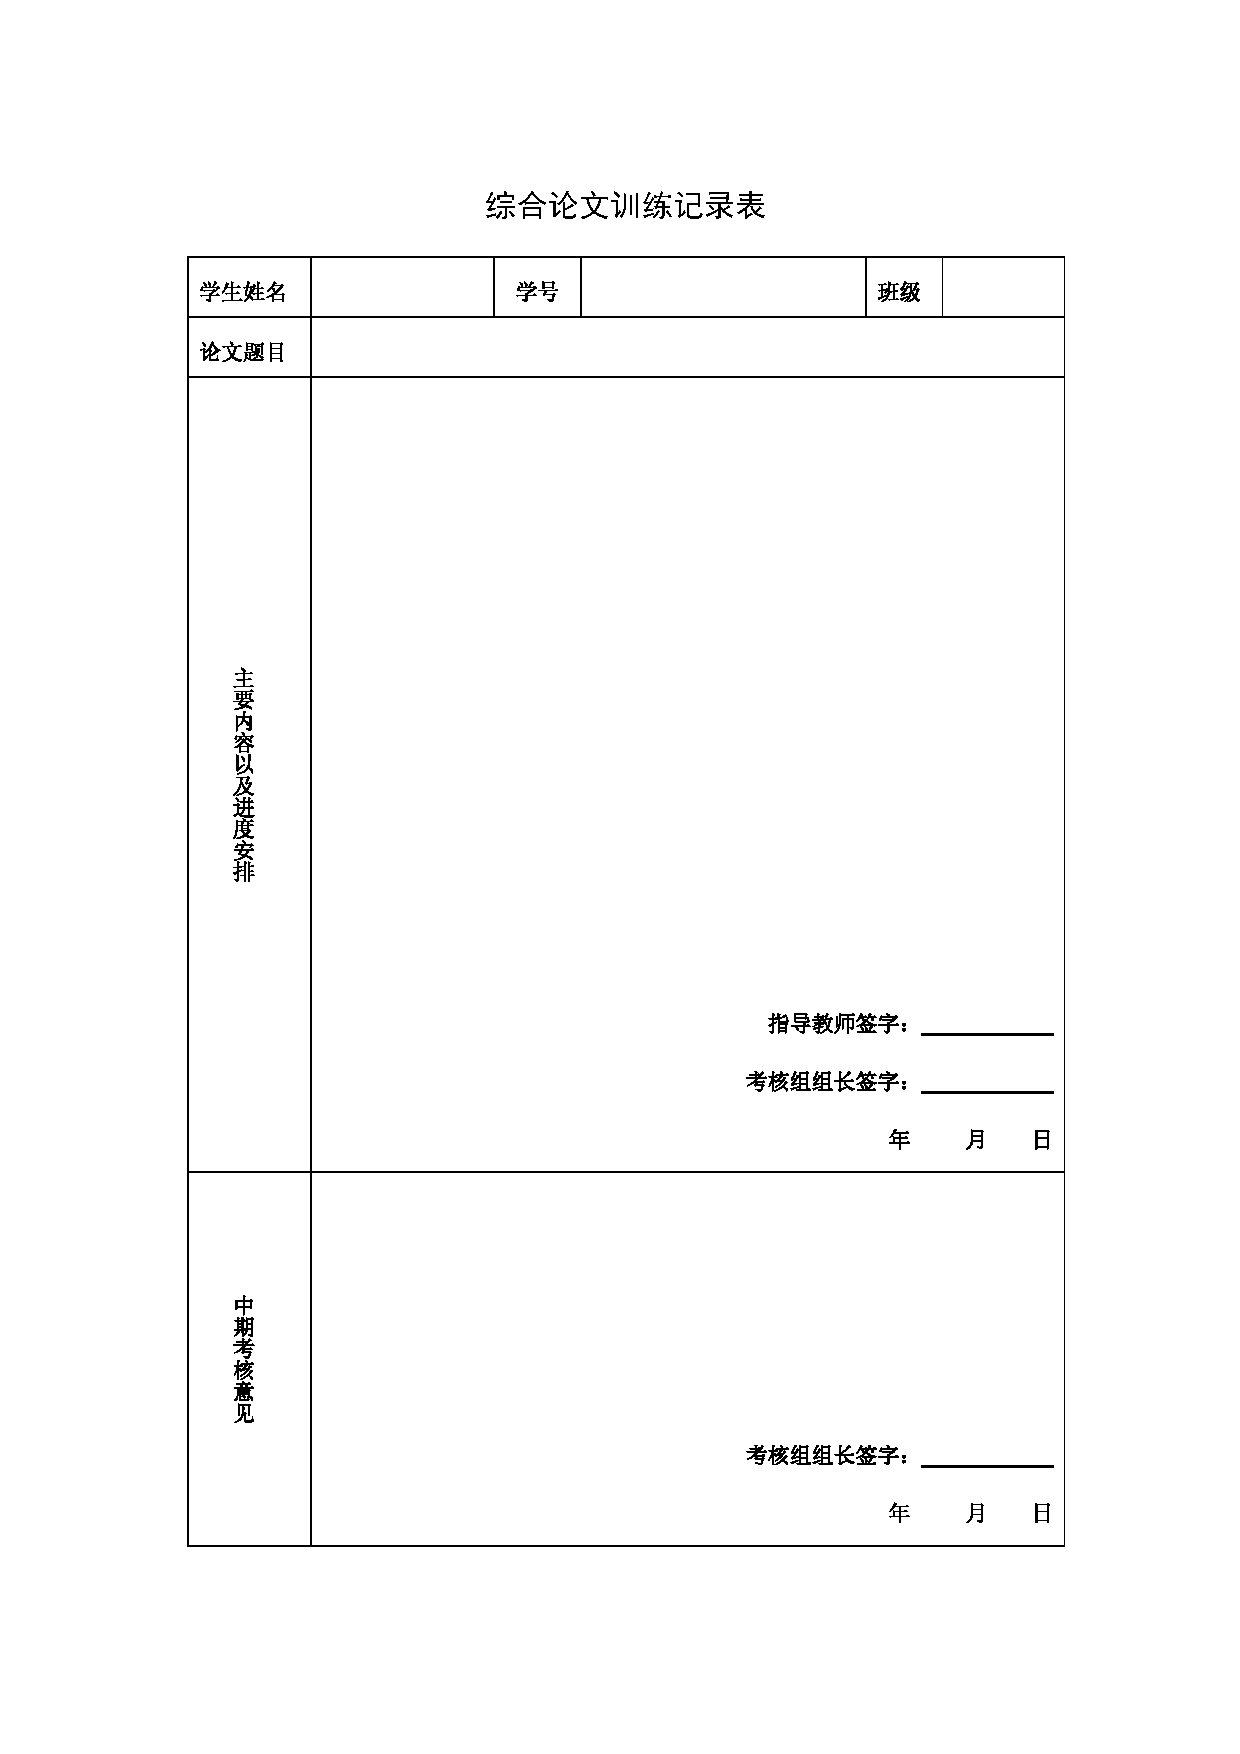
\includepdf[pages=-]{scan-record.pdf}
\end{document}
